%%  -------------------------------------------------------------------------------  %%
%%  Thesis.tex  --  ARCHIVO PRINCIPAL (El que se compila con LaTeX)  %%
%%  -------------------------------------------------------------------------------  %%


%%  -----------------------------------  %%
%%  Configuración del documento  %%
%%  -----------------------------------  %%


\documentclass[a4paper, 11pt, twoside]{Thesis}  % Cambiar twoside por oneside si la impresión no es doble faz.
\graphicspath{{Figures/}}  % Directorio en el que se incluyen los gráficos (deben estar en formato PDF)


%%  ----------------------  %%
%%  Paquetes incluidos  %%
%%  ----------------------  %%


\usepackage[utf8]{inputenc}  % Para codificación de texto UTF8.
\usepackage[spanish]{babel}  % Para escritura en castellano.
\usepackage{graphicx}  % Para manejo de imágenes.
\usepackage{float}  % Para manejo de objetos flotantes.
\usepackage{amsmath}  % Para manejo de expresiones matemáticas.
\usepackage{cancel} % Para poder escribir expresiones canceladas
\usepackage{bigints}  % Para escribir integrales de gra tamaño.
%\usepackage{slashbox}  % Para tablas en las que las cuadrículas se deviden en 2 por una línea obllicua.
\usepackage{bm}  % Para escribir símbolos matemáticos en negrita.
\usepackage{upgreek}  % Para escribir letras griegas rectas.
\usepackage{esint}  % Para usar integrales de superficie.
\usepackage{subfigure}  % Para manejo de subfiguras.
\usepackage{multirow}  % Para realizar tablas con multicolumnas y multifilas.
\usepackage[titletoc]{appendix}
\usepackage{listings}  % Para escritura de código fuente.
\usepackage{textcomp}  % Para incluir símolos especiales en el texto.
\usepackage[framed,numbered,autolinebreaks,useliterate]{mcode}  % Para configurar el color del código de Matlab/Octave (archivo mcode.sty).
\usepackage{color, colortbl}
\usepackage{xcolor}
\usepackage{array,ragged2e}
\usepackage{tabu}


%%  -------------------------------------  %%
%%  Configuración de la bibliografía  %%
%%  -------------------------------------  %%

\usepackage[backend=biber,style=ieee]{biblatex}
\addbibresource{./Bibliography/bibliografia.bib}
\usepackage{csquotes}
%%  ------------------------------  %%
%%  Configuración de los links  %%
%%  ------------------------------  %%


\hypersetup{urlcolor=black, colorlinks=true}  % Muestra los links en negro en todo el documento, no solamente en las referencias.


%%  -------------------------------------  %%
%%  Definición de comandos nuevos  %%
%%  -------------------------------------  %%


\newcommand{\prodesc}{\boldsymbol{\cdot}}  % Producto escalar.
\newcommand{\prodvec}{\boldsymbol{\times}}  % Producto vectorial.
\newcommand{\gradiente}[1]{\nabla#1}  % Gradiente de una curva.
\newcommand{\divergencia}[1]{\nabla\prodesc\mathbf{#1}}  % Divergencia de un vector.
\newcommand{\rotor}[1]{\nabla\prodvec\mathbf{#1}}  % Rotor de un vector.
\newcommand{\laplaciano}[1]{\nabla^2\mathbf{#1}}  % Laplaciano de un vector.
\newcommand{\versor}[1]{\bm{\mathbf{\hat{#1}}}}  % Versor.
\renewcommand{\labelitemi}{$\bullet$}  % Redefine el indicador de ítem en listas no numeradas (1º orden).
\renewcommand{\labelitemii}{\fontsize{4}{4}\selectfont $\blacksquare$}  % Redefine el indicador de ítem en listas no numeradas (2º orden).
\renewcommand{\theequation}{\thechapter\hspace{0.2mm}-\arabic{equation}}  % Coloca un guión entre el cápitulo y el número de ecuación.
\renewcommand{\floatpagefraction}{0.75}
\renewcommand{\appendixname}{Apéndices}
\renewcommand{\appendixtocname}{Apéndices}
\renewcommand{\appendixpagename}{Apéndices}
\addto\captionsspanish{\def\tablename{Tabla} \def\listtablename{\'Indice de tablas}}  % Cambia "cuadro" por tabla e "índice de cuadros" por "índice de tablas".

\newcolumntype{g}{>{\columncolor{black!20}}c} % Para usar columnas grises en tablas de tabu

\hyphenation{dia-gra-ma co-rres-pon-de a-gra-de-ci-mien-to reali-zan-do-se vec-to-rial res-pec-ti-va-men-te elec-tro-mag-ne-tis-mo ver-ti-cal-men-te prin-ci-pio equian-gu-lar me-dian-te es-ta-cio-na-ria pro-pia-men-te con-si-de-ra-cio-nes re-que-ri-mien-to pro-pues-to si-mu-la-cio-nes an-te-na trans-for-ma-dor cons-tru-ir-se fre-cuen-cias fre-cuen-cia exce-len-tes exce-len-te trans-mi-so-ra re-flexio-nes se-miane-coi-ca e-qui-va-len-te li-te-ra-tu-ra de-sa-rro-llo}

\definecolor{Gray}{gray}{0.9}
%%  ------------------------------  %%
%%  Comienzo del documento  %%
%%  ------------------------------  %%


\begin{document}


%%  -----------------------  %%
%%  Portada de la Tesis  %%
%%  -----------------------  %%


\frontmatter  % Enumera las páginas con números romanos.

\title  {Estudio de estructuras de banda prohibida electromagnética (EBG) para la reducción de acoplamiento mutuo entre antenas microstrip}  % Título de la tesis.
\authors  {\texorpdfstring
            {\href{federicoluna@protonmail.com}{Federico Luna}}  % Dirección de mail del tesista en la portada de la tesis.
            {Federico Luna}  % Nombre del tesista.
            }
\addresses  {\groupname\\\deptname\\\univname}  % Editar este campo en el archivo "Thesis.cls".
\date{11 de diciembre de 2017}  % Incluye la fecha al momento de compliar el documento.
\subject{}
\keywords{}
\maketitle

\setstretch{1.3}  % Espacio entre líneas de texto.

\fancyhead{}  % Borra todos los encabezados y notas de pie de página.
\rhead{\thepage}  % Muestra el número de página en la esquina superior derecha.
\lhead{}  % Limpia la esquina superior izquierda.


%%  --------------------  %%
%%  Página con frase  %%
%%  --------------------  %%


\pagestyle{empty}
\null\vfill
\textit{``Study hard what interests you the most in the most undisciplined, irreverent and original manner possible.''}
\begin{flushright}
Richard Feynman
\end{flushright}
\clearpage

\clearpage\pagestyle{empty}\mbox{}\clearpage  % Página en blanco.


%%  ------------------------  %%
%%  Página con resumen  %%
%%  ------------------------  %%


\pagestyle{empty}

\addtotoc{Resumen}  % Agrega "Resumen" al índice.

\abstract

En este trabajo se han estudiado distintos tipos de alimentadores para antenas parabólicas empleando modelos teóricos y simulaciones computacionales. El diseño del alimentador fue realizado a partir de las dimensiones del reflector parabólico construido anteriormente por el autor de la presente tesis. Dicho diseño consiste en una solución de compromiso, la cual establece que la diferencia entre las potencias incidentes en el perímetro y en el vértice del reflector sea aproximadamente -11 dB.

Se han utilizado como alimentador las siguientes antenas: aberturas rectangulares y circulares, guías de onda rectangulares y cilíndricas, y bocinas rectangulares y cónicas.

La construcción del alimentador se realizó a partir de un cilindro de latón que se mecanizó para llegar a las dimensiones que fueron calculadas teóricamente y mediante simulación numérica. La adaptación del alimentador se realizó ajustando la distancia entre el excitador y el cortocircuito de la guía de onda para optimizar la relación de onda estacionaria (ROE).

Respecto a los resultados experimentales, en este trabajo de tesis se han obtenido mejoras en las características del alimentador, particularmente en la radiación posterior (back-scattering) y en el lóbulo principal, en comparación con los alimentadores tradicionales fabricados con guías de onda cilíndricas.

No se registran antecedentes en nuestro país de diseños de estos alimentadores, por lo tanto se estima que va a ser una contribución interesante para la industria local.

\textbf{Palabras clave:} Alimentador, abertura, guía de onda, bocina, reflector parabólico, eficiencia de abertura.

\clearpage

\addtotoc{Abstract}  % Agrega "Abstract" al índice.

\begin{center}
\bigskip{\huge{\textit{Abstract}} \par}\bigskip
\end{center}

The purpose of this investigation was to study different parabolic reflector feeders, using theoretical models and computer simulations. The design of the feeder was made from the dimensions of a parabolic reflector which was previously built by the author of this thesis. Its design is a compromise solution, which establishes that the difference between the incident powers on the reflector's edge and vertex (edge ilumination) is about - 11 dB.

The following antennas have been used as feeders: rectangular and circular apertures, rectangular and cylindrical waveguides, and rectangular and conical horns.

The construction of the feeder was made from a brass cylinder that was turned to obtain the dimensions that were calculated theorically and then by numeric simulation. The feeder matching was made by adjusting the distance between the exciter and the waveguide short to optimize the voltage standing wave ratio (VSWR).

As regards the experimental results in this thesis, improvements have been obtained in the feeder features, specially in the back-scattering radiation and in the main lobe, in comparison with traditional feeders built with cylindrical waveguides.

In our country, there aren't any precedents of these feeders designs', therefore it is estimated that this design will be an interesting contribution to the local industry.

\textbf{Keywords:} Feeder, aperture, waveguide, horn, parabolic reflector, aperture efficiency.

\clearpage


%%  --------------------------------  %%
%%  Página de agradecimientos  %%
%%  --------------------------------  %%


\pagestyle{empty}

\addtotoc{Agradecimientos}  % Agrega "Agradecimientos" al índice.
\begin{center}
\bigskip{\huge{\textit{Agradecimientos}} \par}\bigskip
\end{center}
A mi director de tesis, el Dr. Ing. Walter Gustavo Fano, por toda la dedicación a lo largo del desarrollo de la presente tesis.

Al Ing. Aldo Peruggia, por las licencias del software de simulación FEKO.

Al Ing. Nicolás Tempone, por la ayuda brindada al momento de comenzar y redactar la tesis.

A Rodrigo Carballedo, Omar Fernandez, Ramiro Alonso, Hector Andon y Marcela Luberto, por la buena predisposición, la mano de obra y la ayuda al momento de implementar y medir el alimentador.
\clearpage


%%  ------------------ %%
%%  Índice general  %%
%%  -----------------  %%


\pagestyle{fancy}

\lhead{\emph{Índice general}}
\addtotoc{Índice general}  % Agrega "Índice general" al índice.
\tableofcontents  % Agrega el índice.


%%  -------------------------  %%
%%  Página de dedicatoria  %%
%%  -------------------------  %%


\pagestyle{empty}

\dedicatory{
A mi padre, de quien heredé la vocación por la profesión y que ha sido fundamental a lo largo de estos años para que nunca baje los brazos ante las adversidades, contratiempos y frustraciones.

A mi madre y a mis hermanos, por la confianza, el ánimo y porque han sido pilares fundamentales a lo largo de toda mi carrera.

A Claudia, mi compañera, por la incondicionalidad, su gran paciencia y, sobre todo, por la virtud de poder sacarme una sonrisa hasta en los momentos más difíciles.
}

\addtocontents{toc}{\vspace{2em}}  % Agrega un espacio vertical en el índice, para separar de la enumeración de los capítulos.


%%  ----------------------------------------------------------------------------------  %%
%%  		Aquí comienzan los capítulos, incluyéndolos como archivos separados  		%%
%%  ----------------------------------------------------------------------------------  %%


\mainmatter  % Enumera las páginas con números tradicionales.

\pagestyle{fancy}

\chapter{Introducción: Fundamentos de electromagnetismo}
\label{cap_intro_electro}
\lhead{Capítulo \ref{cap_intro_electro}. \emph{Introducción: Fundamentos de electromagnetismo}} 
%%%%  Las secciones de texto con fórmulas se separan con %%%%
%% Las fórmulas presentes entre 2 secciones de texto se separan con %%

%%%%%%%%%%%%%%%
%%  Capítulo 1: Introducción  %%
%%%%%%%%%%%%%%%

%%%%
\section{Reseña histórica}
\label{sec_intro_resenia}
%%%%

%%%%
Las bases de la teoría electromagnética clásica para el dominio macroscópico fueron formuladas por James Clerk Maxwell en 1873, en base al conocimiento previo desarrollado por Gauss, Ampère y Faraday, entre otros. Entre 1885 y 1887, Oliver Heaviside simplificó las expresiones e introdujo la notación vectorial actual, facilitando así el modelado de guías de ondas y líneas de transmisión \cite{Pozar:MwEngineering}.

En base a estos trabajos, Heinrich Hertz diseñó, entre 1887 y 1891, una serie de experimentos que validaron la teoría de ondas electromagnéticas propuesta por Maxwell. En 1886, Hertz construyó la primer antena dipolo, y en 1888, la primer antena parabólica, alimentada por un dipolo de 450 MHz, dando el puntapié inicial para el desarrollo de la radio durante la primera mitad del siglo \textsc{XX}.

El primer análisis de la propagación de ondas electromagnéticas en guías de ondas metálicas, publicado por Lord Rayleigh en 1897, y el posterior estudio teórico del comportamiento de ondas en guías dieléctricas por Debye y Hondros, en 1910, sentaron los cimientos para que durante la década del '30 comenzaran trabajos experimentales en transporte de ondas electromagnéticas en los laboratorios Bell \cite{Collin:GuidedWaves}.

Los conjuntos de antenas se popularizaron a partir de la aparición de la antena de Yagui-Uda en 1926, formada por elementos lineales que dan lugar a una fase fija. Recién durante la Segunda Guerra Mundial surgieron los conjuntos de antena de fase variable \cite{Stutzman:AntennaTheory}, y las guías de ondas y las antenas tomaron un lugar prioritario entre los ingenieros, matemáticos y físicos de la época, lo que permitió el desarrollo de métodos de análisis para facilitar la formulación de problemas con condiciones de borde complejas.

Recién finalizada la Segunda Guerra Mundial se comenzaron a fabricar circuitos \textit{microstrip}. En 1953, G. A. Deschamps presentó el primer trabajo sobre antenas con la misma tecnología, y la primer patente en ese sentido se registró en 1955 \cite{Balanis:Handbook}. Aún así, recién en la década del '70 comenzaron a utilizarse en aplicaciones prácticas, principalmente debido a la aparición de sustratos con bajas tangentes de pérdida, la mejora en técnicas de fotolitografía, y la optimización de modelos teóricos \cite{Barthia:Handbook}. Sin embargo, la simplificación constructiva trajo aparejados problemas de acoplamiento mutuo, que debieron ser abordados por técnicas de filtrado y blindaje.

%%%%
% NO QUEDÓ BIEN COMPLETO.
%%%%
\section{Ecuaciones de Maxwell}
\label{subsec_ecuaciones_maxwell}
%%%%
La teoría electromagnética propuesta por Maxwell, y simplificada por Heaviside, se reduce a cuatro ecuaciones diferenciales lineales vectoriales e interdependientes que, en notación diferencial, quedan expresadas de la siguiente manera \cite{Pozar:MwEngineering}:

\begin{subequations}
	\label{eq:maxwell_equations}
	\begin{align}	
		\nabla \times \vec{E} & = -\frac{\partial \vec{B}}{\partial t} - \vec{M}  & \text{(Faraday)}\\
		\nabla \times \vec{H} & = \frac{\partial \vec{D}}{\partial t} + \vec{J} & \text{(Ampère)} \label{eq:ampere} \\
		\nabla \cdot \vec{D} & = \rho & \text{(Gauss)} \\
		\nabla \cdot \vec{B} & = 0
	\end{align}
\end{subequations}


donde $\vec{E}$ es el campo eléctrico, en $(V/m)$; $\vec{H}$ es el campo magnético, en $(A/m)$; $\vec{D}$ es la densidad de flujo eléctrico, en $(C/m^2)$; $\vec{B}$ es la densidad de flujo magnético, en $(Wb/m)$; $\vec{M}$ es la densidad de corriente magnética, en $(V/m)$, y se considera por completitud y simetría; $\vec{J}$ es la densidad de corriente eléctrica, en $(A/m^2)$; y $\rho$ es la densidad de carga eléctrica, en $(C/m^2)$.

De las ecuaciones \ref{eq:maxwell_equations} se deduce que las fuentes de campo electromagnético son las corrientes $\vec{M}$ y $\vec{J}$, y la densidad de carga eléctrica $\rho$.

Aplicando la divergencia a la ecuación de Ampere (\ref{eq:ampere}), y recordando que $\nabla \cdot (\nabla \times F) = 0$, se obtiene la ecuación de continuidad, que representa la conservación de la carga, o la continuidad de la corriente, dado que $\nabla \cdot \vec{J}$ representa el flujo de corriente en un punto, y $\partial \rho / \partial t$ representa la variación de la densidad de carga en el mismo punto.

\begin{equation}
	\label{eq:continuidad}
	\nabla \cdot \vec{J} + \frac{\partial \rho}{\partial t} = 0
\end{equation}
%%%%

Dado que la mayor parte del análisis se realiza sobre campos de comportamiento armónico y en régimen permanente, la dependencia del tiempo de la ecuaciones de Maxwell se suele simplificar, y se puede utilizar notación fasorial. Para esto, todos los campos se consideran complejos, y la dependencia temporal, $e^{j \omega t}$, se suele dejar implícita, dado que resulta común para todos los términos. Considerando que cualquier variación en el tiempo físicamente realizable puede ser descompuesta según la transformada de Fourier, no hay pérdida de generalidad al tratar a las ecuaciones de Maxwell de esta manera. Así, las derivadas respecto del tiempo resultan más sencillas, y los vectores de campos se vuelven vectores complejos que son funciones complejas dependientes sólo de coordeanadas espaciales \cite{Collin:GuidedWaves}.

\begin{subequations}
	\label{eq:maxwell_equations_harmonic}
	\begin{align}	
	\nabla \times \vec{E} & = -j \omega \vec{B} - \vec{M} \label{eq:Faraday_harmonic}\\
	\nabla \times \vec{H} & = j \omega \vec{D} + \vec{J} \label{eq:Ampere_harmonic}\\
	\nabla \cdot \vec{D} & = \rho \label{eq:Gauss_harmonic}\\
	\nabla \cdot \vec{B} & = 0
	\end{align}
\end{subequations}

\subsection{Campos en medios materiales}
\label{subsec_campos_en_dielectricos}

Un campo eléctrico aplicado sobre cualquier material dieléctrico genera una polarización de sus átomos y/o moléculas, creando momentos dipolares eléctricos (o alineándolos, si en el material existían previamente), y dando lugar a un vector de polarización adicional, $\vec{P}_e$, que genera un decrecimiento en el campo eléctrico presente en el material. En el mismo sentido, un campo magnético aplicado sobre un medio material podría ser capaz de alinear los momentos dipolares magnéticos en un material magnético, produciendo un vector de polarización magnética $P_m$. Si el medio es, además, lineal e isotrópico, dichas polarizaciones son proporcionales al campo aplicado, de forma que $\vec{P}_e = \epsilon_0 \chi_e \vec{E}$ y $\vec{P}_m = \chi_m \vec{H}$, con $\chi_e$ y $\chi_m$ las susceptibilidades eléctrica y magnética, respectivamente. Dado que las susceptibilidades toman valores complejos, los medios materiales poseen permitividades eléctricas y permeabilidades magnéticas también complejas, por lo que las relaciones constitutivas resultan:
\begin{subequations}
	\label{eq:polarization_vector}
	\begin{align}
		\vec{D} = \epsilon_0 \vec{E} + \vec{P}_e = \epsilon_0 (1+\chi_e)\vec{E} = \epsilon \vec{E} &= \epsilon' - j \epsilon'' \vec{E}\\
		\vec{B} = \mu_0 (\vec{H} + \vec{P}_m) = \mu_0 (1+\chi_m)\vec{H} = \mu \vec{H} &= \mu' - j \mu''\vec{H}
	\end{align}
\end{subequations}

Las partes imaginarias de la permitividad y la permeabilidad ($\epsilon''$ y $\mu''$) representan las pérdidas en el medio debido al amortiguamiento causado por los momentos dipolares respectivos \cite{Fernandez:Electromag}.

Si, además, el material posee una conductividad $\sigma$, la aplicación de un campo eléctrico da lugar a la aparición de una densidad de corriente $\vec{J}$, que en algunos casos, cuando $\sigma$ es independiente del campo eléctrico aplicado, de la dirección del mismo y de la posición, se puede expresar según la ley de Ohm:

\begin{equation}
	\label{eq:ohms_law}
	\vec{J} = \sigma \vec{E}
\end{equation}

La ecuación \ref{eq:ampere} queda, entonces, expresada como
\begin{subequations}
	\begin{align}
		\nabla \times \vec{H} & = j \omega \vec{D} + \vec{J} \\
		& = j \omega \epsilon \vec{E} + \sigma \vec{E} \\
		& = j \omega \epsilon' \vec{E} + (\omega \epsilon'' + \sigma)\vec{E} \\
		& = j \omega \left( \epsilon' - j\epsilon'' - j \frac{\sigma}{\omega} \right) \vec{E}
	\end{align}
\end{subequations}

La relación entre la parte imaginaria y la parte real de la corriente total de desplazamiento se conoce como tangente de pérdidas, definida como \cite{Pozar:MwEngineering}

\begin{equation}
	tan (\delta) = \frac{\omega \epsilon'' + \sigma}{\omega \epsilon'}
\end{equation}

Cuando el material no es homogéneo, los coeficientes $\epsilon$ y $\mu$ dependen de la posición. Si, además, el material es anisotrópico, como en el caso de los cristales y gases ionizados, la relación expresada antes entre los vectores de polarizacón y los campos no se cumplen, sino que deben ser expresadas como tensores de rango 2 (diadas), de manera que quede expresada su dependencia de la dirección \cite{Collin:GuidedWaves}:

\begin{equation}
\begin{bmatrix}
D_x \\
D_y \\
D_z
\end{bmatrix}
=
\begin{bmatrix}
\epsilon_{xx} & \epsilon_{xy} & \epsilon_{xz} \\
\epsilon_{yx} & \epsilon_{yy} & \epsilon_{yz} \\
\epsilon_{zx} & \epsilon_{zy} & \epsilon_{zz}
\end{bmatrix}
\begin{bmatrix}
E_x \\
E_y \\
E_z
\end{bmatrix}
\qquad\text{y}\qquad
\begin{bmatrix}
B_x \\
B_y \\
B_z
\end{bmatrix}
=
\begin{bmatrix}
\mu_{xx} & \mu_{xy} & \mu_{xz} \\
\mu_{yx} & \mu_{yy} & \mu_{yz} \\
\mu_{zx} & \mu_{zy} & \mu_{zz}
\end{bmatrix}
\begin{bmatrix}
H_x \\
H_y \\
H_z
\end{bmatrix}
\end{equation}

Si, además, el material no es lineal, los coeficientes $\epsilon_{ij}$ y $\mu_{ij}$ pueden ser funciones de $\vec{E}$ y $\vec{H}$ respectivamente.
\subsection{Condiciones de borde}

\begin{figure}[htp]
	\centering
	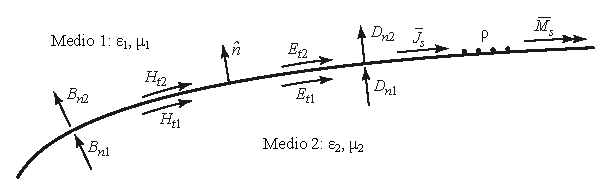
\includegraphics[width=0.8\textwidth]{intro_electro/condiciones_borde.eps}
	\caption{Corrientes, campos y carga superficial en una interfaz general entre dos medios \cite{Pozar:MwEngineering}}
	\label{fig:condiciones_borde}
\end{figure}

Si se considera una interfaz entre dos medios, como la que se muestra en la figura \ref{fig:condiciones_borde}, a partir de las ecuaciones de Maxwell y los teoremas integrales, se pueden deducir las siguientes condiciones de borde:
\begin{subequations}
	\label{eq:condiciones_borde}
	\begin{align}
		\hat{n} \cdot (\vec{D}_{2} - \vec{D}_{1}) & = \rho_s \\
		\hat{n} \cdot (\vec{B}_{2} - \vec{B}_{2}) & = 0 \\
		\hat{n} \times (\vec{E}_2 - \vec{E}_1)  & = - \vec{M}_s \\
		\hat{n} \times (\vec{H}_2 - \vec{H}_1) & = \vec{J}_s
	\end{align}
\end{subequations}

\subsubsection{Campos sobre una superficie dieléctrica}
Dado que en una interfaz entre dos dieléctricos no hay carga eléctrica ni densidades de corriente, las ecuaciones \ref{eq:condiciones_borde} establecen que las componentes normales de los vectores $\vec{D}$ y $\vec{B}$ se conservan, y que las componentes tangenciales de $\vec{E}$ y $\vec{H}$ también lo hacen.

\subsubsection{Campos sobre una superficie conductora eléctrica}
Si el conductor no tiene pérdidas ($\sigma \rightarrow \infty$), todos los campos deben ser cero en su interior, dado que la profundidad de penetración se anula. Considerando, además, que $\vec{M}_s = 0$, la componente tangencial del campo eléctrico, $E_t$ desaparece sobre la superficie del conductor. Dado que la diferencia entre las componentes normales del campo magnético está dada por $\vec{J}_s$, y el campo magnético debe anularse en el conductor, la densidad de corriente superficial está dada únicamente por el campo magnético externo al conductor. En el mismo sentido, la densidad de carga superficial $\rho_s$ es la expresión, sobre la superficie del conductor, de la componente normal de $\vec{D}$.

% SKIN DEPTH

\subsubsection{Campos sobre una superficie conductora magnética}
Dado que la superficie conductora magnética representa el caso dual al de la superficie conductora eléctrica, en este caso se espera que la componente tangencial de $\vec{H}$ se anule sobre la superficie, mientras que la componente tangencial del campo eléctrico dé lugar a corrientes magnéticas sobre la misma.

%%%%% QUEDA DECRI QUE PASA CON UNA CORRIWENTE EN HORIZRAON O VERTICAL - LIBRO DE YAMAT, PAG 10.
%% COMPLETAR CON COLLIN %%

\section{Ecuación de onda}
\label{subsec_eq_de_onda}
%%%%

Al considerar una región del espacio lineal, isotrópica y homogénea, se puede calcular el rotor de la primera ecuación de Maxwell, aplicar la segunda ecuación y, recordando que $\nabla \times \nabla \times \vec{E} = \nabla \nabla \cdot \vec{E} - \nabla^2\vec{E}$, donde $\nabla \times \vec{E} = \rho/\epsilon$, se puede deducir que:

\begin{align}
	\nabla \times \nabla \times \vec{E} & = -j \omega \mu \nabla \times \vec{H} - \nabla \times \vec{M} \notag \\
	\nabla \nabla \cdot \vec{E} - \nabla^2 \vec{E} & = -j \omega \mu \nabla \times \vec{H} - \nabla \times \vec{M} \notag \\
	\frac{\nabla \rho}{\epsilon} - \nabla^2 \vec{E} & = \omega^2 \mu \epsilon \vec{E} - j \omega \mu \vec{J} - \nabla \times \vec{M} \notag\\
	\nabla^2 \vec{E} + \omega^2 \mu \epsilon \vec{E} & = j \omega \mu \vec{J} + \frac{\nabla \rho}{\epsilon} + \nabla \times \vec{M}
	\label{eq:eq_ondas_completa_E}
\end{align}

en el mismo sentido, para el campo magnético:
\begin{align}
	\nabla \times \nabla \times \vec{H} & = j \omega \nabla \times \vec{D} +  \nabla \times \vec{J} \notag \\
	\nabla \nabla \cdot \vec{H} - \nabla^2 \vec{H} & = j \omega \epsilon \nabla \times \vec{E} + \nabla \times \vec{J} \notag \\
	\frac{1}{\mu} \nabla (\cancelto{0}{\nabla \cdot \vec{B}}) - \nabla^2 \vec{H} & = j \omega \epsilon (-j \omega \vec{B} - \vec{M}) + \nabla \times \vec{J} \notag \\
	\nabla^2 \vec{H} + \omega^2 \epsilon \mu \vec{H} & =  j \omega \epsilon \vec{M} - \nabla \times \vec{J}
	\label{eq:eq_ondas_completa_H}
\end{align}

De las ecuaciones anteriores se observa que el campo magnético está determinado por la componente rotacional de la corriente eléctrica, mientras que el campo eléctrico está determinado por todas las componentes de la misma. De manera análoga, se cumple la relación inversa para el caso de la corriente magnética.

Si, además, la región del espacio es libre de fuentes, se deducen las ecuaciones de Helmholtz para ambos campos, donde $k$ es la constante de propagación o número de onda, en unidades de $(1/m)$:

\begin{subequations}
	\label{eq:Helmholtz}
	\begin{align}
		\nabla \times \vec{E} + k^2 \vec{E} = 0 \label{eq:Helmholtz_E} \\
		\nabla \times \vec{H} + k^2 \vec{H} = 0 \label{eq:Helmholtz_H}
	\end{align}
\end{subequations}
%%%%

Para el caso sin pérdidas se puede expresar como $k = \omega \sqrt{\mu \epsilon}$, mientras que si se considera que existen pérdidas óhmicas, las mismas pueden ser tenidas en cuenta si $k$ asume el valor complejo $-j\gamma$, con $\gamma = j\alpha + \beta = j \omega \sqrt{\mu \epsilon} \sqrt{1-j \sigma/(\omega \epsilon)}$. Para el caso de un buen conductor, $\gamma = j\alpha + \beta = j \omega \sqrt{\mu \epsilon} \sqrt{\sigma/(\omega \epsilon)} = (1+j) \sqrt{\omega \mu \sigma/2}$, lo que nos permite definir la profundidad de penetración como $\delta_s = 1/\alpha = \sqrt{2/(\omega \mu \sigma)}$, que decrece con la frecuencia.

En coordenadas cartesianas, la ecuación \ref{eq:Helmholtz_E} se puede escribir como indica la ecuación \ref{eq:Helmholtz_cartesianas_completo}, que además se cumple para todas las coordenadas en que se desarrolla el campo $\vec{E}$. Para cada una de estas coordenadas, resulta sencillo aplicar el método de separación de variables, de forma que $E_i = f(x)g(y)h(z)$ para $i=x, y,$ o $z$, donde las funciones $f(x)$, $g(y)$ y $h(z)$ son independientes.

\begin{equation}
	\label{eq:Helmholtz_cartesianas_completo}
	\nabla^2 \vec{E} + k_0^2 \vec{E} = \frac{\partial^2 \vec{E}}{\partial x^2} + \frac{\partial^2 \vec{E}}{\partial y^2} + \frac{\partial^2 \vec{E}}{\partial z^2} +  k_0^2 \vec{E} = 0
\end{equation}

Sustituyendo, para la ecuación de Helmholtz de cada coordenada, la expresión de $E_i$, se obtiene:

\begin{equation}
	\frac{f''(x)}{f(x)} + \frac{g''(y)}{g(y)} + \frac{h''(z)}{h(z)} + k_0^2 = 0
\end{equation}

Dado que las funciones propuestas son independientes, cada uno de los términos de la ecuación anterior deben dar lugar a una constante:

\begin{equation}
	\frac{f''(x)}{f(x)} = -k_x^2; \qquad \frac{g''(y)}{g(y)} = -k_y^2; \qquad \frac{h''(z)}{h(z)} = -k_z^2
\end{equation}

de manera que:

\begin{equation}
	\label{eq:numero_de_onda}
	k_x^2 + k_y^2 + k_z^2 = k_0^2 \\
\end{equation}

Quedan, entonces, tres ecuaciones diferenciales ordinarias:

\begin{equation}
	\frac{d^2 f}{dx^2} + k_x^2 f = 0; \qquad \frac{d^2 g}{dy^2} + k_y^2 g = 0; \qquad \frac{d^2 h}{dz^2} + k_z^2 h = 0;
\end{equation}

cuyas soluciones son de la forma $e^{\pm j k_i i}$, con $i = x, y$ o $z$, respectivamente. Las soluciones con un signo positivo en el exponente corresponden a ondas que viajan en la dirección negativa ($-x, -y, -z$), mientras que las que tienen un signo negativo corresponden a ondas que viajan en la dirección positiva. Dado que ambas soluciones son válidas y posibles, en función de las condiciones de borde, en general la expresión de un campo $E_i (x, y, z), i=x,y,z$ quedará establecida como la suma de ambas, afectadas por un factor de amplitud dependiente de la coordenada evaluada. Para el caso de ondas que viajan en la dirección positiva:

\begin{equation}
	E_i(x,y,z) = A_i \;e^{-j(k_x x + k_y y + k_z z)}, \quad i=x,y,z
\end{equation}

Lo que indica que la coordenada $i$-ésima del campo eléctrico tendrá un comportamiento exponencial complejo respecto de la posición. 

Si definimos como $\hat{n}$ al versor en la dirección de propagación, podemos definir el vector de número de onda, $\vec{k}$, como:

\begin{equation}
	\label{eq:vector_numero_de_onda}
	\vec{k} = k_x \hat{x} + k_y \hat{y} + k_z \hat{z} = k_o \hat{n}
\end{equation}

De esta forma, se puede expresar, estableciendo $\vec{E}_0 = A \hat{x} + B \hat{y} + C \hat{z}$, y $\vec{r} = x \hat{x} + y \hat{y} + z \hat{z}$, el campo eléctrico como:

\begin{equation}
	\label{eq:electric_field_wave_solution}
	\vec{E} = \vec{E}_0 e^{-j\vec{k} \cdot \vec{r}}
\end{equation}

Para el caso con pérdidas, y considerando que la dirección de propagación es $z$, las componentes $x$ e $y$ se comportan como:

\begin{equation}
E_i(z) = E_i \; e^{-\gamma z} = E_i \; e^{-\alpha z} \; e^{-j \beta z}, \quad i=x,y
\end{equation}

Al expresar la divergencia del campo eléctrico de la ecuación \ref{eq:electric_field_wave_solution}, que en una región sin fuentes es nula, y recordando que $\nabla \cdot (f \vec{A}) = \vec{A} \cdot \nabla f + f \nabla \cdot \vec{A}$, se obtiene:

\begin{align}
	\nabla \cdot \vec{E} = \nabla \cdot \vec{E}_0 e^{-j\vec{k} \cdot \vec{r}} & = \vec{E}_0 \cdot \nabla e^{-j \vec{k} \vec{r}} + e^{-j \vec{k} \vec{r}} \cancelto{0}{\nabla \cdot \vec{E}_0} = 0 \\
	& -j \vec{k} \cdot \vec{E}_0 e^{-j \vec{k} \vec{r}} = 0
\end{align}

De lo que se puede deducir que $\vec{k} \cdot \vec{E}_0 = 0$, de modo que el campo eléctrico, en una onda plana, es siempre perpendicular a la dirección de propagación.

De la ecuación de Faraday (\ref{eq:Faraday_harmonic}), considerando espacio libre de cargas, se puede deducir que el campo magnético es siempre ortogonal al campo eléctrico y a la dirección de propagación, y que los campos están relacionados de forma que \cite{Fernandez:Electromag}:

\begin{equation}
	\vec{H}(\vec{r},t) = \pm \frac{\hat{n} \times \vec{E}(\vec{r},r)}{\eta}
\end{equation}

donde $\eta$ es la impedancia de onda, que tiene la forma $\eta = j \omega \mu / \gamma$. Para el caso del vacío, la impedancia intrínseca se denota $\eta_0$ y tiene un valor de $377\; \Omega$, mientras que para otros materiales está determinada por su permitividad eléctrica y permeabilidad magnética, y puede ser compleja si hay pérdidas.

La velocidad de fase se define como $v_p=\omega/\beta$, que para el caso sin pérdidas queda como $1/\sqrt{\mu \epsilon}$, y que para el caso particular del vacío, se expresa como $1/\sqrt{\mu_0 \epsilon_0} = c$, donde $c$ es la velocidad de la luz en el vacío. Así, la velocidad de fase en cualquier medio material sin pérdidas resulta $c/\sqrt{\epsilon_r \mu_r}$.

La longitud de onda, $\lambda$, es la distancia espacial entre dos máximos sucesivos, por lo que se expresa como $\lambda = 2\pi / k = v_p/f$.

\subsection{Incidencia normal de una onda plana sobre una interfaz}


\subsection{Incidencia oblicua de una onda plana sobre una interfaz}

\section{Guias de ondas}
\label{subsec_guias_de_ondas}
%%%%
LOREM IPSUM
%Pozar, pag 171
%%%%

\subsection{Guía de ondas dieléctricas con plano de tierra}




\section{Líneas de transmisión}
\label{subsec_lineas_de_transmision}
%%%%
LOREM IPSUM
% Venkateswaran, cap 1.
%%%%
\section{Antenas}
\label{subsec_antenas}
%%%%
LOREM IPSUM
%%%%
\subsection{Regiones de campo}
\label{subsubsec_regiones_de_campo}
%%%%
LOREM IPSUM
%%%%
\subsection{Diagramas de radiación}
\label{subsubsec_diag_de_rad}
%%%%
LOREM IPSUM
%%%%
\subsection{Potencia total radiada e intensidad de radiación}
\label{subsubsec_pot_total_radiada}
%%%%
LOREM IPSUM
%%%%
\subsection{Directividad, eficiencia y ganancia}
\label{subsubsec_directividad}
%%%%
LOREM IPSUM
%%%%
\subsection{Polarización}
\label{subsubsec_polarizacion}
%%%%
LOREM IPSUM
%%%%

\subsection{Impedancia de entrada}
\label{subsec_imp_entrada}
%%%%
LOREM IPSUM
%%%%
\subsection{Acoplamiento mutuo}
\label{subsec_acoplamiento}
%%%%
LOREM IPSUM
%%%%
\subsection{Dieléctricos y pérdidas dieléctricas}
\label{subsec_dielectricos}
%%%%
LOREM IPSUM
% LibroSinNombre, pagina 816
%%%%
\subsection{Parámetros S}
\label{subsec_parametros_s}
%%%%
LOREM IPSUM
% Pozar, pag 178
%%%%

\subsection{Antenas Microstrip}
\label{subsec_antenas_microstrip}
%%%%
LOREM IPSUM
%%%%
\subsubsection{Modelo de líneas de transmisión}
\label{subsubsec_microstrip_modeloLineas}
%%%%
LOREM IPSUM
% LibroSinNombre, pahgina 534
%%%%
\subsubsection{Modelo de cavidades multimodo}
\label{subsubsec_microstrip_modeloCavidades}
%%%%
LOREM IPSUM
% Pozar, rezonadores, capitulo 6
%%%%

\subsection{Acoplamiento mutuo en antenas Microstrip}
\label{subsec_acoplamiento_microstrip}
%%%%
LOREM IPSUM
%%%%
% LibroSinNombre, pagina 562 y 631
\subsubsection{Ondas de superficie}
\label{subsubsec_microstrip_ondas_superficie}
%%%%
LOREM IPSUM
%%%%
% Engheta, pagina 289
% Rahim (tesis), pagina 28
% Collin, capitulo de Surface waveguides, pag 697
% Paper de Barlow.
% Pozar, pag 138
% Tesis de Kovacs, pagina 8
% Tesis de Zheng, apendice A, pag 48. Interfaces con diel y con metales.



\chapter{Fundamentos de estructuras de EBG}
\label{cap_fundamentos}
\lhead{Capítulo \ref{cap_fundamentos}. \emph{Fundamentos de EBG}} 
%%%%%%%%%%%%%%%%%%%%%%%%%%
%%  Capítulo 2: Fundamentos de estructuras de banda prohibida electromagnética (EBG)}  %%
%%%%%%%%%%%%%%%%%%%%%%%%%%

%%%%
\section{Reseña histórica: Metamateriales, materiales periódicos y EBGs}
\label{sec_resenia_metamateriales}
%%%%
% EBGs in Antennas, Rahmat (libro). Pagina 2.
% Explicación de los métodos de análisis
% Uso para low profile antennas
% Engheta, pag 215
% Caloz, ^pag 17
% Caloz Pag 20
% Caloz pag 83, diferencia con filtros
% Pozar, pag 380
% Pozar, p 424. Stepped impedance filters.
% Pozar, bandstop filter design, pag 440
% Tabla interesante: Baccarello, Paulotto, impreso.
% stack de capas o cristal? Brown, McMahon, Parker. Ademas linda foto.
% Relación con soft-hard surfaces. Gao, chen, wang, yang-
% Discusión terminológica: Oliner.
% ITOH, Pediodic structures.
% DGS, tesis de ABIDIN, pag2. Tiene intro histórica.
% ABIDIN, tesis, pagina 16: Def de EBG. imagen interesante.
% Venkateswaran, algunos ejemplos de EBGs.
% Importancia de EBGs. Venkateswaran tesis, pag 1.
% Algo de intro: Pagina 4, tesis Zheng.
\lipsum
\section{Difracción de Bragg}
\label{sec_bragg}
%%%%
% Caloz, pag 19
% Kamgaing (tesis), pagina22
\lipsum
\section{Bloch-Floquet}
\label{sec_bloch}
%%%%
\lipsum
% Libro de rahmat. Pagina 46.
% Zona de brillouin. Rahmat, libro, pagina 31.
% Diagrama de dispersión. Página 67 Rahmat. Caloz: pagina 106.
% Impedancia de Bloch: Caloz, pagina 113
% Tesis Choi, pag 82.
% Tesis Kovacs, pag 13.
% Venkateswaran, pag 26.
% Tesis Zheng, pag 5-8
\section{Impedancia de onda y de superficie}
\label{sec_imp_superficie}
%%%%
% Rahmat. Pagina 77 libro.
% Engheta, pagina 290.
\lipsum


\section{Metamateriales ópticos: Cristales fotónicos}
\label{sec_cristales_fotonicos}
%%%%
\lipsum
% Lightline stuff. Rahmat, pagina 28. Caloz, pagina 139. Pozar pag 386
\section{Tipos de EBG}
\label{sec_tipos_mtm}
%%%%
\lipsum[1]
% Tesis de kovacs, pagina 7.
\subsection{EBGs de mano izquierda}
\label{subsec_ebg_izquierda}
%%%%
\lipsum
% Caloz, Pag 27, 43, 
\subsection{EBGs uniplanares}
\label{subsec_ebg_uniplanar}
%%%%
\lipsum
% buena intro en rahmat (libro), pagina 35-37
% Buscar las distintas formas, incluyendo Peano. Relación con FSS.
% Buena intro esn Goussetis, Feresidis, Vardaxoglou.
% Diseños para incidencia obliucua: Kim, Yand, Elsherbeni. Tambien en Lin, Li, Zhang.
% Hilbert: McVAy, Engheta, Hoorfar.
% Power loss analysis: Mohajer-Iravani, Ramahi, de Hindawi corp.
% Kern, Douglas, Werner.
% Analisis en Goussetis, Feresidis, paper posta. Tipos de resonancia.
% Lamminen, Vimpari, Saily. 
% Maci, Caiazzo, Cucini. Jodido, interesante. Leer.
\section{Modelado y simulación de metamateriales}
\label{sec_simulacion_mtm}
%%%%
\lipsum
% Un modelado medio simple se puede ver en la tesis de Choi, pag 90-99
\subsection{Métodos de cavidades periódicas}
\label{subsec_eigenfunctions}
%%%%
\lipsum
% Fullwave: Baccarello, Paulotto, impreso.
% Hacer estudio gráfico similar al CALOZ, pag 176.
\subsection{Modelado por líneas de transmisión}
%%%%
\lipsum
% Caloz, pag 60, 67, 76, 79
% Bidimensional, Caloz, pag 133
% Rahman Stuchly.ç
% Calculo de la inductancia de meander inductors: Stojanovic, Zivanov
% Cuentas! Wu, Lin, Wang, Wang, Chen
% Kim, Schutt-Ainé, 178. Modelado para PDN.
%Venkateswaran, pag 40 en adelante.
% Impedancia: hacer algo similar. Tesis Zheng, pag 8

\subsubsection{TMM}
%%%%
\lipsum[2]
% Caloz, pagina 144
% Choi (tesis), pag 54
\subsubsection{TLM}
\label{subsubsec_tlm}
%%%%
\lipsum
% Caloz, pag 155

\chapter{Estudio y diseño de estructuras de banda prohibida electromagnética}
\label{cap_modelado}
\lhead{Capítulo \ref{cap_modelado}. \emph{Estudio y diseño de estructuras de banda prohibida electromagnética}}
%%%%%%%%%%%%%%%%%%%%%%%%%
%%  Capítulo 3: Modelado y simulacion de metamateriales  %%
%%%%%%%%%%%%%%%%%%%%%%%%%

%%%%
\section{Análisis de estructuras periódicas}
\label{sec_estructuras_periodicas}
%%%%
\lipsum
% Libro de rahmat. Pagina 59.
%%%%
\section{Análisis de estructuras planares propuestas}
\label{sec_estructuras_propuestas}
%%%%
\lipsum
\lipsum
% Comentar cómo se logró periodicidad, vinculando las fases.
%%%%
\section{Estudio de estructuras mediante TLM}
\label{sec_estudio_tlm}
%%%%
\lipsum
\lipsum
%Pasos: Barchloui: Simulation of FSS surfaces using 3d TLM, 2003. Primer paper de un librito. Buena explciaci{on.}
% Paper importante: Hoefer 1985. Johns, 1971.
% Leer Janyani, Paul, TLM modelling of nonlinear optical effects in fibre bragg gratings, 2004.
% Kim Kim Kang, Yook: Modeling and analysis of ebg in power distribution networks.
% sadiku

%%%%
\subsection{Algoritmo utilizando programación orientada a objetos}
\label{subsec_estudio_tlm}
%%%%
\lipsum

\chapter{Aplicación de EBGs en estructuras microstrip}
\label{cap_aplicacion}
\lhead{Capítulo \ref{cap_aplicacion}. \emph{Aplicación de EBGs en estructuras microstrip}}
%%%%%%%%%%%%%%%%%%%%%%%
%%  Capítulo 4: Aplicación a estructras microstrip  %%
%%%%%%%%%%%%%%%%%%%%%%%

%%%%

\section{Introducción}

El análisis del capítulo 3 permite comprender de forma intuitiva el comportamiento de las estructuras EBG uniplanares dispuestas sobre un plano de tierra cubierto por sustrato dieléctrico. Sin embargo, el análisis sólo se propuso para energía conducida, debida al comportamiento de corrientes sobre el metamaterial que dan lugar a una modificación en la estructura y capacidad de propagación de ondas. Este análisis, si bien importante para la comprensión de los efectos ligados a las estructuras periódicas, no se centra en el análisis del comportamiento de las mismas en cercanías de radiadores electromagnéticos.

En este capítulo se iniciará, aunque no se concluirá completamente, el estudio sobre el efecto de estas estructuras sobre las propiedades de radiación y de campo cercano de antenas ubicadas sobre el sustrato. El análisis comenzará con la revisión del comportamiento cuando las antenas en cuestión son monopolos eléctricos referenciados al plano conductor inferior, y una vez destacados los efectos más importantes que se dan para este tipo de antenas, se procederá a mostrar los efectos para el caso en que los radiadores son antenas \textit{microstrip}, en que aparecen fenómenos más complejos.

El motivo por el que se comienza el análisis para monopolos eléctricos verticales gira en torno a la capacidad que estos poseen para generar, sobre la capa dieléctrica, ondas de superficie TM en forma isotrópica, sin efectos de borde ni asimetrías que dificulten el análisis.

\section{Elección del metamaterial}
\label{sec_eleccion}

Existen numerosas posibles celdas unitarias uniplanares, que fueron creadas a partir de la propuesta inicial de Yang y otros \cite{Yang:UCPBG}, y que procuran aumentar el ancho de banda prohibida y el valor de atenuación, muchas veces utilizando técnicas de miniaturización, que buscan lograr geometrías que presenten una mayor o menor inductancia, y una mayor o menor capacidad con el plano de tierra y con celdas vecinas, en función de las necesidades. La búsqueda, en el contexto de la disminución del acoplamiento mutuo entre antenas \textit{microstrip}, de celdas unitarias óptimas, gira alrededor de la búsqueda de anchos de banda prohibidos lo suficientemente amplios para cubrir el ancho de banda de las antenas \textit{microstrip} en cuestión.

Para este trabajo se seleccionó la celda de Yang, analizada en la sección \ref{sec:celda-yang}, debido a que fue la primer variante publicada, y posee optimizaciones sobre la celda de Orlandi, analizada en la sección \ref{sec:celdas-orlandi}.

Sin embargo, existen numerosos diseños y geometrías, entre las que destacan la celda analizada por Goussetis \cite{Goussetis:TailoringAMCEBGCharacteristics}, que consiste en parches cuadrados sin interconexión entre sí, como el mostrado en la figura \ref{fig:rectangulo-cuadrado}. Si bien, debido a su geometría, estas celdas unitarias presentan capacidad con el plano de tierra y con otros parches aledaños, presentan una baja inductancia, lo que los vuelve subóptimos, dado que resulta complejo obtener frecuencias de resonancia lo suficientemente bajas con un tamaño de celda viable. Otros trabajos de interés son los de Abidin \cite{Abidin:Thesis}, quien propuso las estructuras mostradas en las figuras \ref{fig:abidin1} y \ref{fig:abidin2}, que poseen un ancho de banda mayor al de las celdas de Yang, aunque requieren más iteraciones de simulación, debido a la complejidad de las geometrías.

Estructuras más sencillas son propuestas en \cite{Asimonis:designoptimization}, mostradas en las figuras \ref{fig:assimonis1}, \ref{fig:assimonis2} y \ref{fig:assimonis3}, con resultados similares a la geometría elegida en este trabajo.

Entre los esfuerzos más intuitivos para aumentar la inductancia, disminuyendo así la frecuencia de resonancia y, por tanto, el tamaño de las celdas unitarias, se destaca el propuesto por \cite{IslamAlam:CompactEBG}, mostrado en la figura \ref{fig:islamalam}. En ella se observa que se aumentó el largo y la capacidad de las cintas \textit{microstrip} que unen los parches, modificando las líneas para que ocuparan la mayor cantidad de espacio posible. Las simulaciones de esta estructura ofrecen mejores resultados que los de la celda elegida, aunque al costo de dificultar su diseño en programas \textsc{CAD}. Un modelo utilizando líneas de transmisión para caracterizar el comportamiento de estas celdas está presentado en \cite{Venkateswaran:Thesis}. 

En este sentido, \cite{Kovacs:DesignOptimization} propone, en su tesis doctoral, un algoritmo genético capaz de obtener un mayor ancho de banda prohibida mediante sucesivas simulaciones, sin la intervención de un diseñador, obteniendo celdas complejas pero muy efectivas, como la mostrada en la figura \ref{fig:kovacs}.


\begin{figure}[h]
	\centering 
	\subfigure[Celda unitaria propuesta por \cite{Abidin:Thesis}.]{
		\label{fig:abidin1}
		\includegraphics[width=0.30\textwidth]{Aplicacion/abidin1.png}}
	\hspace{30pt}
	\subfigure[Celda unitaria propuesta por \cite{Abidin:Thesis}.]{
		\label{fig:abidin2}
		\includegraphics[width=0.30\textwidth]{Aplicacion/abidin2.png}}
	\subfigure[Celda unitaria propuesta por \cite{Asimonis:designoptimization}.]{
		\label{fig:assimonis1}
		\includegraphics[width=0.30\textwidth]{Aplicacion/assimonis1.png}}
	\hspace{30pt}
	\subfigure[Celda unitaria propuesta por \cite{Asimonis:designoptimization}.]{
		\label{fig:assimonis2}
		\includegraphics[width=0.30\textwidth]{Aplicacion/assimonis2.png}}
	\subfigure[Celda unitaria propuesta por \cite{Asimonis:designoptimization}.]{
		\label{fig:assimonis3}
		\includegraphics[width=0.30\textwidth]{Aplicacion/assimonis3.png}}
	\hspace{30pt}
	\subfigure[Celda unitaria propuesta por \cite{IslamAlam:CompactEBG}.]{
		\label{fig:islamalam}
		\includegraphics[width=0.30\textwidth]{Aplicacion/islamalam.png}}
	\subfigure[Celda unitaria propuesta por \cite{Kovacs:DesignOptimization}.]{
		\label{fig:kovacs}
		\includegraphics[width=0.30\textwidth]{Aplicacion/kovacs.png}}
	\caption{Variación del parámetro $S_{11}$ del puerto en función de distintos parámetros del parche único, y antena optimizada final.}
	\label{fig:posibles-geometrias}
\end{figure}

La miniaturización cumple un papel importante debido a que es necesaria una cantidad (o profundidad) mínima de celdas unitarias entre los parches para que el efecto de disminución de acoplamiento resulte notorio. Si cada una de las celdas unitarias ocupara demasiada superficie, obligaría a separar los parches aún más, consecuencia que resulta indeseable. Además, entre la estructura de celdas unitarias y los parches se debe mantener una distancia $g$ mínima, de modo que los efectos de acoplamiento de campo cercano entre la antena y la estructura EBG puedan considerarse despreciables. Estos efectos no son despreciables y, en muchos casos, generan un acoplamiento aún mayor al que se da si no se utilizan estructuras EBG.

Para el caso de una distancia entre los parches de aproximadamente $3\lambda/2$, la cantidad de filas de celdas unitarias que se pueden ubicar entre los mismos para observar efectos de atenuación del acoplamiento mutuo varía entre 3 y 5. Las técnicas de modelado presentadas, y en particular las que requieren de simulación de una celda unitaria y la aplicación de condiciones de borde periódicas, describen el comportamiento de la estructura EBG cuando ésta se extiende infinitamente. Como, en general, este no es el caso, se procedió, utilizando como base la información brindada por los diagramas de dispersión (que en nuestro caso, debido a que la cantidad de celdas unitarias es finita, describen en forma aproximada las zonas frecuencia de atenuación), a obtener la relación del parámetro $S_{21}$ con la frecuencia para distintos valores geométricos, simulando la estructura completa.

De los parámetros analizados que describen la geometría de las celdas unitarias de Yang, para ambos análisis (el que corresponde a la resolución de una única celda unitaria con condiciones de contorno periódicas, el del parche central y la distancia entre los parches de dos celdas unitarias aledañas.

En general, un mayor tamaño de celda da lugar a una banda de atenuación ubicada a frecuencias más bajas. La elección gira en torno a que la frecuencia de resonancia del sistema sobre el que se desea probar el comportamiento de la estructura se ubique en una zona segura ante problemas y tolerancias de fabricación.

\section{Monopolos}

Las antenas monopolo consisten en un conductor dispuesto verticalmente sobre un plano de tierra u otra superficie conductora, alimentado o conectado a un receptor en su base a través de una línea de transmisión cuyos terminales están conectados al plano de tierra y al conductor vertical respectivamente, como se muestra en la figura \ref{fig:monopolos} b). A diferencia del dipolo, que consiste en dos conductores idénticos dispuestos de forma tal que comparten su eje principal, el monopolo suele ser más corto, posee un diagrama de radiación más elevado (como se observa en la figura \ref{fig:monopolos} a)), una resistencia de radiación menor, una mayor directividad, y da lugar a ondas de superficie considerables sobre el plano conductor.


\begin{figure}[H]
	\centering 
	\subfigure[Diagrama de radiación de un monopolo de longitud $2\lambda/3$.]{
		\label{fig:diag-rad-monopolo}
		\includegraphics[width=0.30\textwidth]{Aplicacion/diagrad-monopolo-wikipedia.jpg}}
	\hspace{30pt}
	\subfigure[Diagrama de una antena monopolo.]{
		\label{fig:monopolo}
		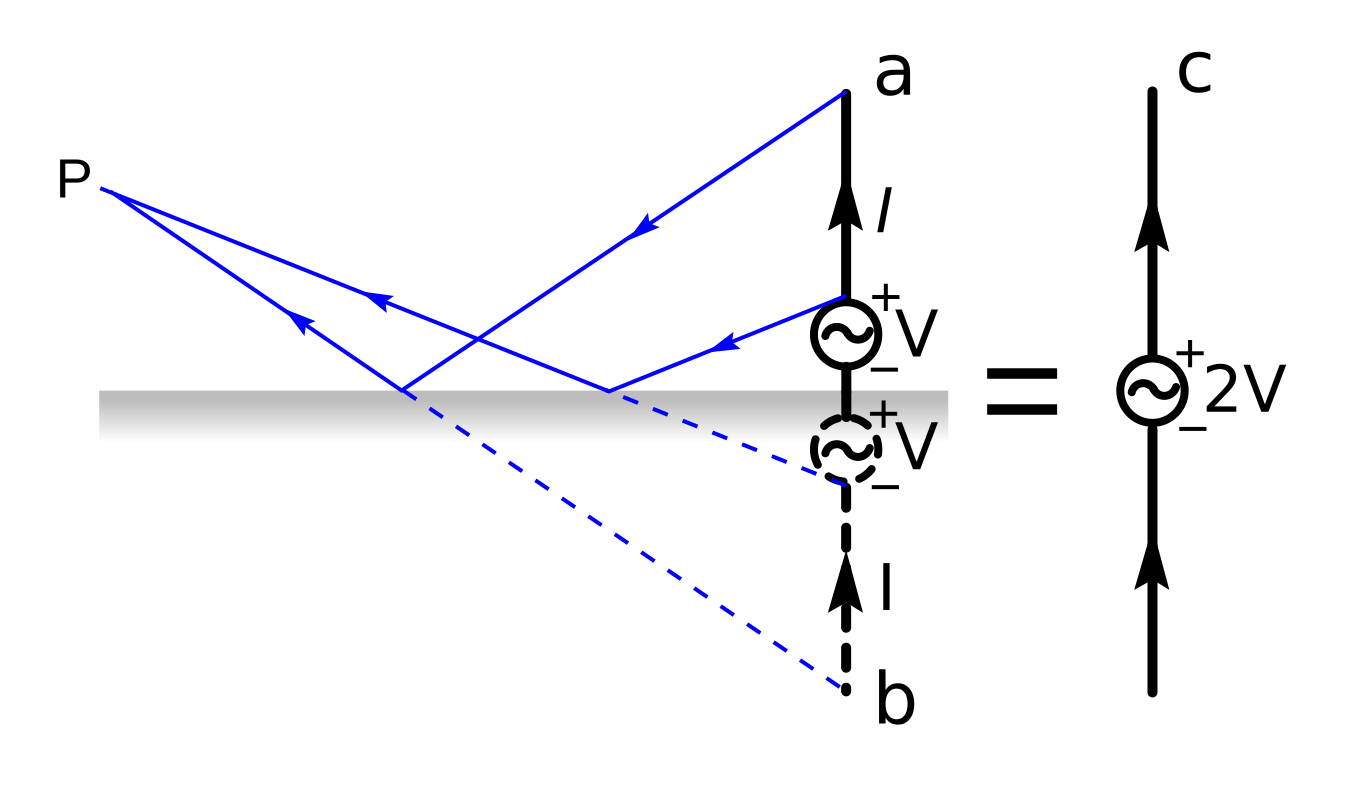
\includegraphics[width=0.50\textwidth]{Aplicacion/Monopole_and_image_antenna.pdf}}
	\caption{Imágenes extraídas de \textit{Wikipedia}.}
	\label{fig:monopolos}
\end{figure}


El análisis de un monopolo suele derivar de la aplicación de teoría de imágenes sobre un dipolo dispuesto a cierta distancia del plano de tierra. Este método de análisis genera fuentes virtuales de radiación bajo el plano conductor que, combinadas con las fuentes reales (el conductor vertical del monopolo), dan lugar a un sistema equivalente para la zona del espacio que se ubica por encima del plano de tierra, dado que describe las reflexiones sobre el mismo. Las fuentes virtuales tienen, sobre un plano conductor, el comportamiento mostrado en la figura \ref{fig:fuentes-virtuales}.


\begin{figure}[h]
	\centering
	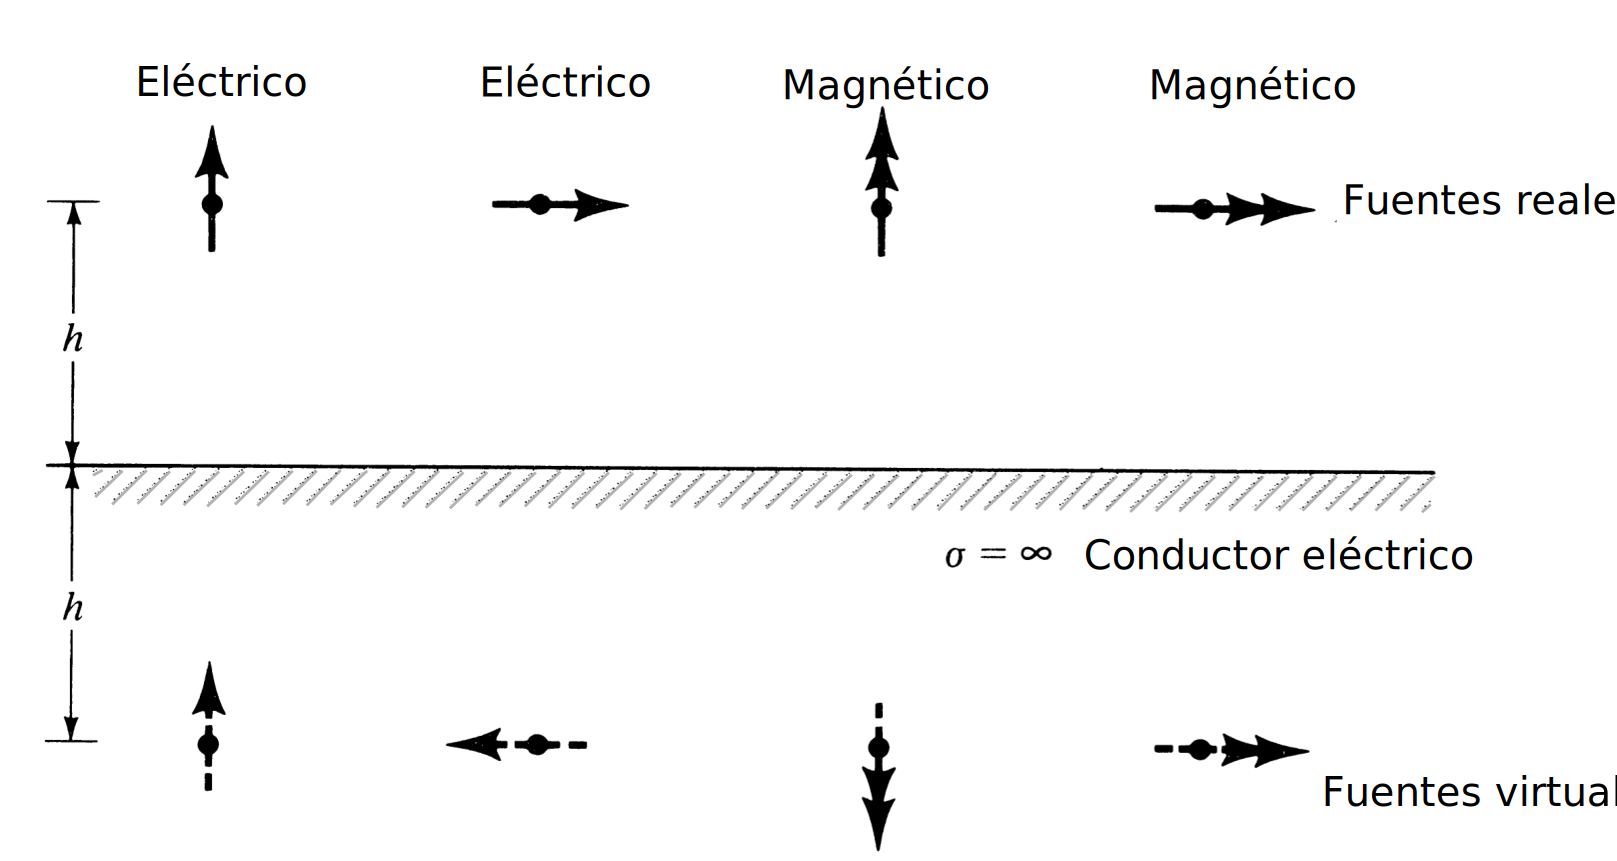
\includegraphics[width=1\textwidth]{Aplicacion/balanis-metodo-imagenes.PNG}
	\caption{Fuentes virtuales generadas por cercanía con un conductor eléctrico \cite{Balanis:Theory}.}
	\label{fig:fuentes-virtuales}
\end{figure}

\subsection{Comportamiento de un arreglo de dos monopolos}

Para las pruebas sobre acoplamiento mutuo que se realizaron, se consideró un monopolo de $\lambda/4$, que para la frecuencia de interés es de aproximadamente $3.125\;cm$. Se ubicaron dos monopolos a una distancia arbitraria de $6.25\; cm$ sobre un plano conductor finito cubierto por un sustrato de FR-4, a fin de conocer el acoplamiento entre ambas antenas cuando no existe una estructura de \textit{bandgap} electromagnético entre ellas. La geometría creada se puede observar en la figura \ref{fig:dos-monopolos}. Se debe considerar que, como se explicó en la sección \ref{subsec_acoplamiento}, el acoplamiento entre antenas se debe a múltiples factores, y el uso de estructuras EBG en el sustrato será responsable de únicamente uno de ellos: las ondas de superficie.

\begin{figure}[h]
	\centering
	\includegraphics[width=0.7\textwidth]{Aplicacion/dos-monopolos.png}
	\caption{Estructura de dos monopolos sobre un plano de tierra simulada.}
	\label{fig:dos-monopolos}
\end{figure}

Por el motivo antes comentado, si las antenas se ubicaran demasiado cerca, la intensidad relativa de los efectos debidos al acoplamiento por campo cercano serían mucho mayores a los del acoplamiento por ondas de superficie, de forma que en muchos casos, en lugar de mejorar el comportamiento, el uso de EBGs lo empeorará, sumando más efectos negativos que positivos. Estas estructuras resultarán útiles sólo en aquellos casos en que la distancia entre los radiadores sea lo suficientemente grande como para poder considerar efectos de acoplamiento relacionados a la propagación de ondas de superficie.

Se varió la distancia para conocer la variación del coeficiente de acoplamiento con la misma. Los resultados se muestran en la figura \ref{fig:dipolos-distancia-resultados} donde, como resultaba esperable, el mismo disminuye con la distancia, y la frecuencia de resonancia del mismo aumenta ligeramente a medida que los dipolos se alejan, modificando de forma casi insignificante el nivel de adaptación.

\begin{figure}[h]
	\centering 
	\subfigure[Parámetro $S_{11}$.]{
		\label{fig:dipolos-s11-variasDistancias-sinEBG}
		\includegraphics[width=0.45\textwidth]{Aplicacion/dipolos-s11-variasDistancias-sinEBG.pdf}}
	\hspace{0pt}
	\subfigure[Parámetro $S_{12}$.]{
		\label{fig:dipolos-s12-variasDistancias-sinEBG}
		\includegraphics[width=0.45\textwidth]{Aplicacion/dipolos-s12-variasDistancias-sinEBG.pdf}}
	\caption{Comportamiento de los parámetros S para dos dipolos ubicados a distintas distancias.}
	\label{fig:dipolos-distancia-resultados}	
\end{figure}  

En vistas de comprender la incidencia del acoplamiento por ondas de superficie sobre el acoplamiento total entre ambas antenas, se eliminó el plano de tierra que se ubica entre ambos dipolos. Esto tiene consecuencias muy notorias sobre el diagrama de radiación, pues deja de existir el plano conductor y, por tanto, la fuente de campo virtual que se consideraba en la figura \ref{fig:monopolos} b) ya no existe. El comportamiento del parámetro $S_{21}$ para el caso en que no hay un plano de tierra completo que vincule a ambas antenas se pueden observar en la figura \ref{fig:monopolos-sin-plano-de-tierra-resultados}, que surge de la simulación de la figura \ref{fig:monopolos-sin-plano-de-tierra-geometria}. 


\begin{figure}[h]
	\centering
	\includegraphics[width=0.5\textwidth]{Aplicacion/dos-monopolos-sin-GND.png}
	\caption{Estructura de dos monopolos ubicados sobre dos planos conductores separados para evitar acoplamiento por ondas de superficie.}
	\label{fig:monopolos-sin-plano-de-tierra-geometria}
\end{figure}

\begin{figure}[h]
	\centering 
	\subfigure[Parámetro $S_{11}$.]{
		\label{fig:dipolos-s11-variasDistancias-sinGND}
		\includegraphics[width=0.45\textwidth]{Aplicacion/dipolos-s11-variasDistancias-sinGND.pdf}}
	\hspace{0pt}
	\subfigure[Parámetro $S_{12}$.]{
		\label{fig:dipolos-s12-variasDistancias-sinGND}
		\includegraphics[width=0.45\textwidth]{Aplicacion/dipolos-s12-variasDistancias-sinGND.pdf}}
	\caption{Comportamiento de los parámetros S para dos dipolos ubicados a distintas distancias, con un plano de tierra dividido en dos para evitar acoplamiento por ondas de superficie.}
	\label{fig:monopolos-sin-plano-de-tierra-resultados}	
\end{figure}  

Se puede observar que los valores de distancia para los que los monopolos quedan cerca del borde de su respectivo plano conductor y del radiador opuesto, la adaptación del sistema mejora considerablemente. A medida que las antenas se alejan, el parámetro $S_{11}$ recupera los valores que poseía cuando la estructura tenía un único de plano de tierra. Una comparación para dos distancias elegidas arbitrariamente se puede observar en la figura \ref{fig:comparacion-monopolos-s-sinGND} a). De la misma manera, el comportamiento en función de la frecuencia de las geometrías en que la distancia entre los monopolos, y entre cada uno de los radiadores y el borde del plano conductor, disminuye, el acoplamiento aumenta para las bajas frecuencias, y surgen efectos indeseados. Una comparación, también para dos distancias elegidas arbitrariamente, se observa en la figura \ref{fig:comparacion-monopolos-s-sinGND} b), donde se puede observar una disminución en el parámetro $S_{12}$ de unos $8\ dB$ para las frecuencias de interés, incluso cuando las antenas están lejos del borde que las enfrenta (curva naranja). Esto permite deducir, entonces, que el efecto de acoplamiento por ondas de superficie no es despreciable, aunque no representa, como se esperaba, la causa única del mismo.


\begin{figure}[h]
	\centering 
	\subfigure[Parámetro $S_{11}$.]{
		\label{fig:comparacion-dipolos-s11-variasDistancias-sinGND}
		\includegraphics[width=0.45\textwidth]{Aplicacion/comparacion-dipolos-s11-variasDistancias-sinGND.pdf}}
	\hspace{0pt}
	\subfigure[Parámetro $S_{12}$.]{
		\label{fig:comparacion-dipolos-s12-variasDistancias-sinGND}
		\includegraphics[width=0.45\textwidth]{Aplicacion/comparacion-dipolos-s12-variasDistancias-sinGND.pdf}}
	\caption{Comparación del comportamiento entre un par de monopolos que comparten plano conductor y un par de dipolos que no, para dos distancias entre antenas elegidas arbitrariamente.}
	\label{fig:comparacion-monopolos-s-sinGND}
\end{figure} 


La aplicación de estructuras EBG modifica sustancialmente las características de las antenas. En la figura \ref{fig:parametros-s-2ebg} se puede observar el comportamiento de los parámetros $S$ para el caso en que entre las dos antenas se ubican dos filas de EBG, como se muestra en la figura \ref{fig:estructuras2-y-3-ebg-monopolos} a). Se observa que a una menor distancia entre los dipolos y, por lo tanto, entre cada dipolo y la estructura EBG, el comportamiento es más errático, aunque la adaptación es más profunda. En el mismo sentido, el acoplamiento entre las antenas disminuye con la distancia, y una menor distancia al EBG de cada dipolo genera un acoplamiento mayor al original.

\begin{figure}[h]
	\centering 
	\subfigure[Parámetro $S_{11}$.]{
		\label{fig:parametros-s-2ebg-s11}
		\includegraphics[width=0.45\textwidth]{Aplicacion/dipolos-s11-variasDistancias-conEBG.pdf}}
	\hspace{0pt}
	\subfigure[Parámetro $S_{12}$.]{
		\label{fig:parametros-s-2ebg-s21}
		\includegraphics[width=0.45\textwidth]{Aplicacion/dipolos-s12-variasDistancias-conEBG.pdf}}
	\caption{Comportamiento de los parámetros $S$ para monopolos separados por dos filas del EBG propuesto.}
	\label{fig:parametros-s-2ebg}
\end{figure}

\begin{figure}[h]
	\centering 
	\subfigure[Dos filas de EBG.]{
		\label{fig:estructuras2-ebg-monopolos}
		\includegraphics[width=0.45\textwidth]{Aplicacion/dos-monopolos-2EBG.png}}
	\hspace{0pt}
	\subfigure[Tres filas de EBG.]{
		\label{fig:estructuras3-ebg-monopolos}
		\includegraphics[width=0.45\textwidth]{Aplicacion/dos-monopolos-3EBG.png}}
	\caption{Estructuras simuladas de dos monopolos separados por 2 y 3 filas de celdas de EBG.}
	\label{fig:estructuras2-y-3-ebg-monopolos}
\end{figure} 

Una comparación entre los parámetros $S$ para el caso con y sin 2 filas de celdas de EBG se puede observar en la figura \ref{fig:comparacion-2filas-ebg-mo}. La misma revela que, cuando se ubican los EBG, incluso para el caso en que están separados una distancia considerable de los monopolos, la frecuencia de resonancia disminuye considerablemente. Esto obliga a considerar a la estructura EBG al momento del diseño de las antenas.

Como se explicitó antes, en ocasiones el uso de EBG con la intención de disminuir el acoplamiento mutuo entre antenas monopolo genera un acoplamiento aún mayor entre las mismas, efectivamente generando el efecto contrario al buscado. Esto se observa en la figura \ref{fig:comparacion-2filas-ebg-mo} b). Para la mayor parte de la banda del espectro de interés, el parámetro $S_{12}$ de las antenas es mayor cuando se utilizan dos filas de EBG dispuestas entre las antenas que cuando no. Sin embargo, en una banda angosta cercana a la frecuencia de resonancia de los EBG, el parámetro $S_{12}$ disminuye fuertemente, a valores unos $15\; dB$ por debajo del caso en que no se interpone la estructura. Vale aclarar que, en base al análisis y modelado previo, se esperaba un ancho de banda de rechazo mucho mayor. Cuando la estructura está lo suficientemente lejos, el aumento del acoplamiento en la banda de interés es menos notorio, aunque no despreciable, y la disminución del valor de $S_{21}$ en la frecuencia de resonancia del EBG resulta de alrededor de $10\; dB$.

\begin{figure}[h]
	\centering 
	\subfigure[Parámetro $S_{11}$.]{
		\label{fig:comparacion-2filas-ebg-mo-s11}
		\includegraphics[width=0.45\textwidth]{Aplicacion/comparacion-dipolos-s11-variasDistancias-sinConEBG.pdf}}
	\hspace{0pt}
	\subfigure[Parámetro $S_{12}$.]{
		\label{fig:comparacion-2filas-ebg-mo-s12}
		\includegraphics[width=0.45\textwidth]{Aplicacion/comparacion-dipolos-s12-variasDistancias-sinConEBG.pdf}}
	\caption{Comparación del comportamiento de los parámetros $S$ para el caso en que no hay EBG y el caso en que se ubican dos filas de celdas.}
	\label{fig:comparacion-2filas-ebg-mo}
\end{figure} 

El caso en que se ubican 3 EBG, los resultados, que se muestran en la figura \ref{fig:comparacion-3filas-ebg-mo}, son más complejos. La frecuencia de resonancia disminuye fuertemente, y aparecen resonancias cercanas que dificultan la adaptación. Este comportamiento patológico es mucho menos notorio a medida que la distancia entre los monopolos y la estructura disminuye. En el caso del parámetro $S_{12}$, aparecen también frecuencias de resonancia cercanas a la que corresponde al comportamiento de las celdas EBG, aunque, de igual manera que para el caso del parámeteo $S_{11}$, los efectos desaparecen al alejar los monopolos de la estructura.

\begin{figure}[h]
	\centering 
	\subfigure[Parámetro $S_{11}$.]{
		\label{fig:comparacion-3filas-ebg-mo-s11}
		\includegraphics[width=0.45\textwidth]{Aplicacion/dipolos-s11-variasDistancias-con3EBG.pdf}}
	\hspace{0pt}
	\subfigure[Parámetro $S_{12}$.]{
		\label{fig:comparacion-3filas-ebg-mo-s12}
		\includegraphics[width=0.45\textwidth]{Aplicacion/dipolos-s12-variasDistancias-con3EBG.pdf}}
	\caption{Comportamiento de los parámetros $S$ para monopolos separados por tres filas del EBG propuesto.}
	\label{fig:comparacion-3filas-ebg-mo}
\end{figure}

La comparación entre el comportamiento para 2 y 3 filas de celdas EBG se puede observar en la figura \ref{fig:comparacion-23filas-ebg-mo}, para dos distancias. Para el caso $S_{11}$, se puede observar fácilmente que la frecuencia de resonancia es menor y el comportamiento en frecuencia es mucho más errático, con múltiples resonancias que afectan a la adaptación. Cuando la distancia es mayor, esas resonancias disminuyen y la diferencia entre el uso de 2 y 3 filas de celdas EBG disminuye. Los valores de adaptación mejoran ligeramente para el caso de 3 filas, pero a costa de una disminución en la frecuencia. El parámetro $S_{12}$ para el caso de monopolos a $7.6\; cm$ de distancia entre sí presenta picos que generan que el valor alcance los $-10\;dB$, aunque cuando los mismos se alejan a $10.6\;cm$, a pesar de que resuena a menores frecuencias, se observa una disminución del parámetro en $20\; dB$ en una banda angosta centrada por debajo de la frecuencia en que se deseaba disminuir el acoplamiento.

\begin{figure}[h]
	\centering 
	\subfigure[Parámetro $S_{11}$.]{
		\label{fig:comparacion-23filas-ebg-mo11}
		\includegraphics[width=0.45\textwidth]{Aplicacion/comparacion-dipolos-s11-variasDistancias-conEBG2-3.pdf}}
	\hspace{0pt}
	\subfigure[Parámetro $S_{12}$.]{
		\label{fig:comparacion-23filas-ebg-mo12}
		\includegraphics[width=0.45\textwidth]{Aplicacion/comparacion-dipolos-s12-variasDistancias-conEBG2-3.pdf}}
	\caption{Comparación del comportamiento de los parámetros $S$ para el caso en que no hay EBG y el caso en que se ubican dos filas de celdas.}
	\label{fig:comparacion-23filas-ebg-mo}
\end{figure} 

	
\section{Introducción a antenas \textit{microstrip}}

Como se describió en la sección \ref{subsec_antenas_microstrip}, las antenas \textit{microstrip} son utilizadas en un amplio rango de aplicaciones comerciales y militares, especialmente debido a que son livianas, de bajo perfil, suponen reducidos costos y resultan de fácil fabricación. Además, permiten diseños integrados con componentes activos, circuitos de microondas y elementos radiantes \cite{Yang:EBGAntennas}.

El tamaño de las antenas está íntimamente ligado a la longitud de onda de trabajo, que se relaciona a la frecuencia y permitividad eléctrica del sustrato utilizado, como queda explícito en la ecuación \ref{eq:frecRes-modosSup-microstripAntenna}. Al mismo tiempo, dado que en general son antenas resonantes, presentan un alto Q, lo que afecta a su ancho de banda.

En muchos casos es necesario disminuir el tamaño de los elementos \textit{microstrip}, lo que se puede lograr mediante cortocircuitos y líneas \textit{microstrip} de formas complejas. Otro método, más sencillo, consiste en aumentar el valor de la permitividad eléctrica del sustrato. Sin embargo, como ya se explicó antes, y como se puede observar en la figura \ref{fig:zstm-permit-diel}, el aumento de este parámetro aumenta el valor de la impedancia inductiva de la superficie, permitiendo el desarrollo de ondas de superficie.

Por otro lado, el uso de dieléctricos de constante alta genera un ancho de banda aún menor (un mayor Q) y aún más baja eficiencia de radiación. Estos efectos suelen mitigarse con el aumento del ancho del sustrato, que, en contrapartida, genera condiciones propicias para la propagación de ondas de superficie en modo TM, debido a que, como se indica en la ecuación \ref{eq:campo-magnetico-interior-diel-TM} y se esquematiza en la figura \ref{fig:soluciones-TM-tan-implicita-zoom}, se permiten una mayor cantidad de modos de propagación en el eje $x$ (vertical). Por otro lado, un análisis de la impedancia de superficie indica que el comportamiento inductivo aumenta con el ancho del sustrato (ecuación \ref{eq:impedancia-superficie-tm-teorica} y figura \ref{fig:Zstm-parametros}), lo que también es signo de una configuración que soporta ondas de superficie con facilidad.

Las ondas de superficie, además, extraen potencia que no se convierte en radiación y, facilitan el acoplamiento entre elementos. Además, cuando inciden sobre discontinuidades, generan lóbulos secundarios que degradan el patrón de radiación y las características de polarización \cite{Balanis:Theory}.

Entre las distintas técnicas que han surgido para la disminución de la presencia de ondas de superficie en el sustrato que soporta a las antenas \textit{microstrip}, entre las que destacan las relativas a disminuir la altura del sustrato en los bordes de la antena (figura \ref{fig:escalon-sustrato}), en los últimos años ha cobrado especial interés el uso de sustratos con banda prohibida electromagnética, debido a que no requieren un cambio en la tecnología de fabricación. Los mismos pueden aplicarse justo debajo de la antena (generando estructuras planares que reemplazan al plano de tierra, conocidas como DGS, que ofrecen como contrapartida un diagrama de radiación con mayores lóbulos laterales), o alrededor de la misma (\cite{Marcela:Tesis}, figura \ref{fig:sustrato-antena-ebg}). Ambas soluciones, debido a la naturaleza resonante de la antena, que genera que las frecuencias en juego estén distribuidas en un ancho de banda acotado, tienen como consecuencia una disminución del acoplamiento mutuo con elementos circuitales cercanos a la antena (en particular, otras antenas que podrían estar formando parte de un arreglo de radiadores). Esto es así porque, si las estructuras que rodean al elemento radiante tienen una banda prohibida para las frecuencias de trabajo, las mismas no podrán propagarse por el sustrato.


\begin{figure}[H]
	\centering 
	\subfigure[Antena rodeada por una estructura EBG.]{
		\label{fig:sustrato-antena-ebg}
		\includegraphics[width=0.40\textwidth]{Aplicacion/foto-ebg-alrededor-antena.pdf}}
	\hspace{30pt}
	\subfigure[Antena rodeada por un escalón de sustrato,]{
		\label{fig:escalon-sustrato}
		\includegraphics[width=0.40\textwidth]{Aplicacion/foto-escalon-alrededor-antena.pdf}}
	\caption{Fotos de diseños de antenas parches con limitadores a la propagación de onda de superficie \cite{Yang:EBGAntennas}.}
	\label{fig:limitadores-ondas-superficie-yang}
\end{figure}

Las primeras estructuras EBG utilizadas con estos fines consistían en arreglos de agujeros cilíndricos en el sustrato que, debido a la periodicidad que presentaban para las ondas de superficie, daban lugar a un comportamiento de filtro, presentando una banda prohibida. La dificultad para la fabricación de este tipo de sustratos dio lugar a la búsqueda de estructuras de banda prohibida de mayor facilidad de uso. En 1999, Sievenpiper presentó, en sus tesis doctoral \cite{Sievenpiper:Thesis}, una estructura que denominó HIS (\textit{High Impedance Surface}, superficie de alta impedancia), que además de cumplir con las características de un conductor magnético para un rango de frecuencias \cite{Sievenpiper:HIESForbiddenBand} y de ser de fácil fabricación con tecnología \textit{microstrip}, poseía también una banda prohibida electromagnética para las ondas de superficie \cite{Marcela:Tesis}. Esta estructura, consistente en parches metálicos dispuestos sobre un sustrato, y unidos al plano de tierra, ubicado en la cara opuesta del mismo, a través de vías metálicas, redujo ampliamente los costos y la dificultad de fabricación. Pocos años más tarde, debido a que en algunos casos el uso de vías retrasa la fabricación de circuitos \textit{microstrip}, surgieron estructuras de banda prohibida uniplanares, con características similares, aunque con anchos de banda prohibida más reducidos.

Para el presente trabajo, estas estructuras se ubicarán entre dos antenas \textit{microstrip}, alineadas según distintos criterios, a fin de comparar el diagrama de radiación y el acoplamiento mutuo con el que se logra con el mismo arreglo radiante, pero sin el uso de EBG entre ellas.

% Coccioli, Yang, Itoh, intro historica.
%%%%
\section{Diseño de una antena \textit{microstrip}}
\label{sec_disenio_microstrip}
%%%%
Para el diseño de una antena \textit{microstrip}, se deben utilizar los modelos teóricos analizados en la sección \ref{sec:modelo_analitico}. Se debe calcular, en primer lugar, un valor tentativo del ancho W de la antena (con W según la figura \ref{fig:antema-microstrip-inset} a)), teniendo en cuenta que un mayor ancho W da lugar a una menor resistencia de entrada $R_{in}$. Una fórmula empírica está dada por \cite{Barthia:Handbook}, y para una frecuencia de resonancia de unos 2.42 GHz y sustrato FR-4 de 1.6 mm de espesor, resulta:

\begin{align}
	W = \frac{c_0}{2 f_r} \sqrt{\frac{2}{\epsilon_r+1}} = 37.35\; mm.
\end{align}

Obtenido el ancho aproximado, se puede calcular la permitividad eléctrica eficaz, $\epsilon_{eff}$, de la ecuación \ref{eq:cte-diel-efectiva-microstrip}, que resulta 4.17. Esto permite, conociendo la frecuencia de resonancia buscada, calcular la longitud efectiva de la línea de transmisión, como:

\begin{align}
	L_{eff} = \frac{c_0}{2 f_r \sqrt{\epsilon_{r_{eff}}}} = 30.32\; mm.
\end{align}

Dado que $L_{eff} = L + 2 \Delta L$, a partir del cálculo de $\Delta L$, que cuantiza el efecto del \textit{fringing} sobre la frecuencia de resonancia, usando la expresión \ref{eq:deltaL-antena-microstrip}, que resulta en 0.74 mm, se puede saber el valor de L a utilizar ($L = L_{eff} - 2 \Delta L$), que es de 28.85 mm.

Además de la antena, debe diseñarse también la alimentación de la misma. De entre las múltiples formas de alimentación de una antena \textit{microstrip} \cite{Barthia:Handbook}, la seleccionada, en este trabajo, por su facilidad de fabricación, es la que consiste en una línea de la misma tecnología, que vincula a un conector en el borde de la placa con el parche, esquematizado antes en la figura \ref{fig:antema-microstrip-inset}. En particular, es importante que la impedancia característica de la línea \textit{microstrip} utilizada sea de $50\;\Omega$, para lo que debe seleccionarse con cuidado su ancho, en función de la altura del sustrato y la permitividad del dieléctrico. Según las expresiones que se pueden hallar en el Apéndice B de \cite{Barthia:Handbook}, el ancho necesario para obtener una impedancia de $50\;\Omega$ es de aproximadamente 3.1 mm.

Conocidos estos valores, resta determinar el \textit{inset} que debe aplicarse para obtener una impedancia de entrada de 50 $\Omega$, a fin de lograr adaptación entre la línea \textit{microstrip} de alimentación y el parche radiante. Para esto, se debe utilizar la curva de la figura \ref{fig:antema-microstrip-inset} b), conociendo previamente el valor de la impedancia sobre el borde del parche rectangular. A partir de las expresiones de la parte real de la admitancia, o conductancia, obtenidas de \cite{Balanis:Theory} y mostradas en las ecuaciones \ref{eq:conductancia-microstrip-balanis} (donde $J_0$ es una función de Bessel del primer tipo de orden cero), la resistencia de entrada resulta $R_{in} = 1/[2(G_1 \pm G_{12})]$. A partir de este valor, la consulta a la gráfica permite deducir que el valor de \textit{inset} requerido es de aproximadamente 10.73 mm.

\begin{align}
	\label{eq:conductancia-microstrip-balanis}
	G_1 &= \frac{1}{\pi \eta_0} \int_0^\pi \left[ \frac{\sin \left( \frac{k_0 W}{2} \cos \theta \right) }{\cos \theta}\right]^2 \sin^3 \theta d\theta, \\
	G_{12} &= \frac{1}{120 \pi^2} \int_0^{\pi} \left[ \frac{\sin \left( \frac{k_0 W}{2} \cos \theta \right) }{\cos \theta}\right]^2 J_o(k_0 L \sin \theta) \sin^3 \theta d\theta.
\end{align}

El siguiente paso consiste en describir geométricamente la estructura calculada para el uso de un software de simulación que permita optimizar los parámetros, en vistas de que la frecuencia de resonancia sea 2.41 GHz, y que el parámetro $S_{11}$, correspondiente al puerto de alimentación, sea tan pequeño como sea posible. Es importante aclarar que el agregado de los parches de carga y de la estructura EBG modificará la frecuencia de resonancia, y que este análisis se realiza en miras de comprender los cambios que se producen sobre la antena original, y confirmar el aumento de ancho de banda mediante la técnica mencionada antes.

Los resultados de la variación de los tres parámetros de interés en el diseño de la antena, ya elegido el sustrato, se observan en la figura \ref{fig:simulaciones-microstrip-1parche}. Como se puede observar, en efecto de la variación del largo L es muy notorio, debido a que, como se explicó antes, modifica la frecuencia de resonancia: A mayor largo L, menor resulta la frecuencia de resonancia, debido a que la longitud de onda en resonancia es más corta. Se observa que para alrededor de 45 mm de largo, la frecuencia de resonancia ronda la buscada.

\begin{figure}[H]
	\centering 
	\subfigure[Variación del largo L.]{
		\label{fig:1parche-varlargo}
		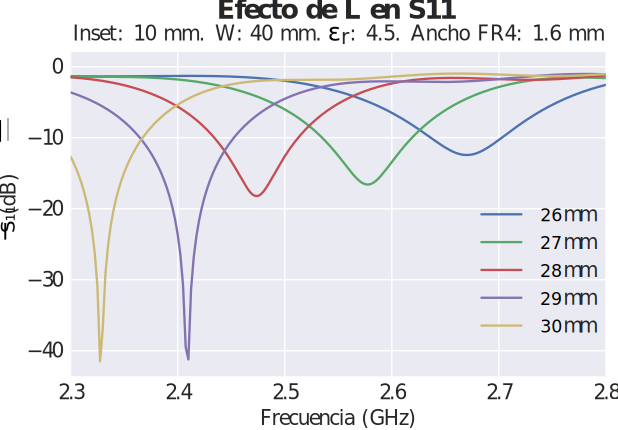
\includegraphics[width=0.48\textwidth]{Aplicacion/VariacionLargo-UnParche.pdf}}
	\subfigure[Variación del ancho W.]{
		\label{fig:1parche-varancho}
		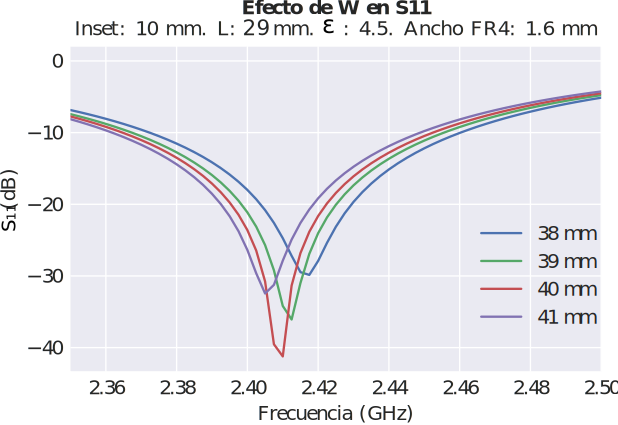
\includegraphics[width=0.48\textwidth]{Aplicacion/VariacionAncho-UnParche.pdf}}
	\subfigure[Variación de valor del \textit{inset}.]{
		\label{fig:1parche-varinset}
		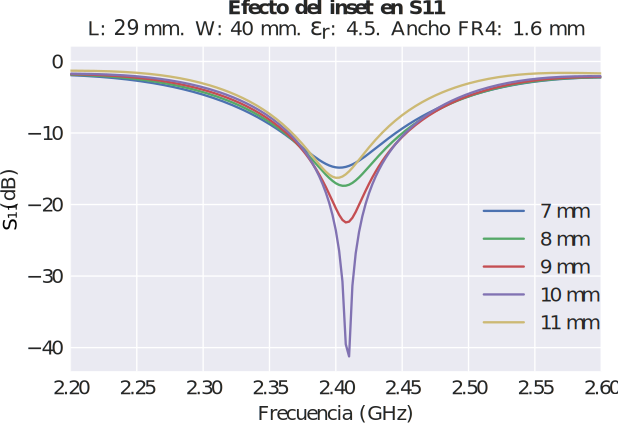
\includegraphics[width=0.48\textwidth]{Aplicacion/VariacionInset-UnParche.pdf}}
	\hspace{19pt}
	\subfigure[Antena sin cargas optimizada.]{
		\label{fig:antena-optimizada}
		\includegraphics[width=0.42\textwidth]{Aplicacion/antena-optimizada.PNG}}
	\caption{Variación del parámetro $S_{11}$ del puerto en función de distintos parámetros del parche único, y antena optimizada final.}
	\label{fig:simulaciones-microstrip-1parche}
\end{figure}

La variación del valor del ancho W produce efectos menos notorios, modificando ligeramente la frecuencia de resonancia debido a que tiene impacto sobre la longitud efectiva del parche. Además, como se explicó previamente, el ancho del parche modifica la resistencia de entrada, lo que modifica  los valores de $S_{11}$, haciendo que para valores cercanos a 40 mm se obtenga el valor óptimo.

Finalmente, el parámetro de más fácil modificación manual en un parche, el valor del \textit{inset}, da lugar a variaciones muy grandes en el valor del parámetro $S_{11}$. Esto permite una fácil adaptación manual de la antena. Se observa que el valor de \textit{inset} de aproximadamente 10 mm genera los resultados deseados.

La optimización de los parámetros geométricos, realizada con CST Microwave Studio, con objetivo en establecer los valores más adecuados automáticamente para lograr el mínimo valor de $S_{11}$ en 2.41 GHz, arrojó como resultado un valor de L de 28.86 mm, un valor de W de 40.41 mm y un valor de \textit{inset} de 9.59 mm, como se indica en la figura \ref{fig:antena-optimizada}.

En miras de comparar el efecto sobre el campo lejano de las modificaciones a realizarse sobre el parche para aumentar el ancho de banda, se muestra, en la figura \ref{fig:farfield-1parche-sincarga-sinebg}, el comportamiento en campo lejano, donde se asume un sustrato de 190 mm $\times$ 135 mm.

\begin{figure}[h]
	\centering
	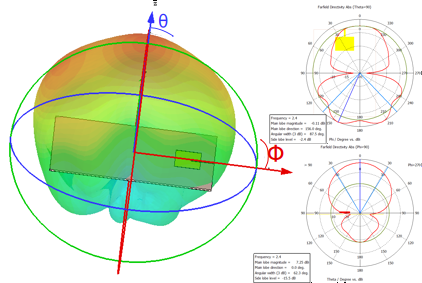
\includegraphics[width=1\textwidth]{Aplicacion/FarfieldResults.pdf}
	\caption{Comportamiento del campo lejano para un parche \textit{microstrip} sin modificaciones, en la frecuencia de resonancia. La imagen tridimensional izquierda muestra la estructura y, en colores, el valor de la directividad para cada dirección. Además, muestra la dirección de variación de $\theta$ y $\phi$. La gráfica superior derecha representa, en rojo, la variación de la directividad en función de $\phi$, para un $\theta$ de $90^{\circ}$, es decir, rasante al plano de la antena. La gráfica inferior derecha representa la variación de la directividad en función de $\theta$, para un valor de $\phi$ de $90^{\circ}$.}
	\label{fig:farfield-1parche-sincarga-sinebg}
\end{figure}


Para poder estudiar este problema, será necesario comprender cómo se comporta un conjunto de dos antenas \textit{microstrip} sin estructuras entre ellas, separadas una distancia adecuada para que los efectos de acoplamiento mutuo resulten visibles. Para evitar, tanto como sea posible, el acoplamiento debido a fenómenos no relacionados a la propagación de ondas de superficie, se debe ubicar a los elementos radiantes a una distancia tal que el diagrama de radiación tenga un comportamiento \textit{broadside}, es decir, que el lóbulo principal del diagrama de radiación tenga dirección perpendicular al plano de tierra. Para esto, la distancia entre las antenas debe ser múltiplo impar de $\lambda_g/2$, donde $\lambda_g$ es la longitud de onda en el sustrato (FR-4, en nuestro caso), donde se considera un valor de $\epsilon_{eff}$ de 4.17. Este valor de permitividad modifica la velocidad de las ondas electromagnéticas, de modo que la longitud de onda, para la frecuencia de resonancia $f_r$ de la antena \textit{microstrip}, es menor a la del vacío. En nuestro caso:

\begin{align}
	\label{eq:lambdag}
	\lambda_g = \frac{v_p}{f_r} = \frac{c}{\sqrt{\epsilon_{eff} f_r}} \approx 60.9\; mm.
\end{align}

Considerando que se debe dejar espacio entre las antenas para que se pueda ubicar una estructura EBG entre ellas, se decidió que la distancia entre las mismas resulte de $\frac{3}{2} \lambda_g = 91.35\;mm$.

% Simulaciones en el trabajo.

%% COMO ES ESA DISTANCIA??

% Simular, incluyendo farfield.

% PONER FOTO
% Poner resultados finales

% Condiciones de borde: LIbroSinNombre, pagina 398.
%%%%

\section{Diseño de un conjunto de dos antenas \textit{microstrip}}
\label{sec_conjunto}
El diseño de una única antena microstrip representa el primer paso en la obtención de un conjunto capaz de aumentar la directividad, y por tanto la ganancia, de la estructura. Lamentablemente, la simple utilización de los valores calculados en la sección \ref{sec_disenio_microstrip} no ofrece, en general, buenos resultados. Esto se debe a que las antenas que conforman el conjunto se deben disponer a distancias tales que modifican el espacio circundante a cada una de ellas, generando acoplamiento indeseados y variaciones en la frecuencia de resonancia y los parámetros de adaptación. Es por esto que la sección precedente sólo ofrece valores aproximados a los que se utilizan en el diseño final.

En miras de la obtención de resultados simulados que contemplen las posibilidades de fabricación de un conjunto de dos antenas \textit{microstrip} separadas una distancia de $3/2 \lambda$, se simularon las mismas considerando un sustrato de 135 mm $\times$ 190 mm, de forma que las mismas se ubican a corta distancia del borde de la placa de sustrato utilizada, como se muestra en la figura \ref{fig:conjunto-sin-ebg}. En la misma, los valores de alto, ancho y valor de \textit{inset} de las antenas son iguales, y fueron elegidos tras la simulación a valores cercanos a los obtenidos en la sección anterior. Estos valores, mostrados en la tabla \ref{table:valores-dosparches-geometria}, serán los utilizados para la comparación con las geometrias radiantes con estructuras de banda prohibida electromagnética. En la figura \ref{fig:farfield-2parches-sinebg} se puede observar el diagrama de radiación tridimensional para la estructura propuesta, con las dimensiones elegidas.

\begin{table}
	\centering
	\begin{tabular}{c|c|c|c|c}
		$L$ & $W$ & $y_0$ & $w_{linea}$ & $s$ \\
		\hline
		$31$ mm & $38$ mm & $11$ mm & $3$ mm & $91.35$ mm
	\end{tabular}
	\caption{Tabla de valores elegidos para los parches que conforman al arreglo de dos antenas \textit{microstrip}.}
	\label{table:valores-dosparches-geometria}
\end{table}

GeometriaconjuntoSinEBG.png

FarField3D-DosParches-SinEBG
FarField2D-phifijo-DosParches-SinEBG





\section{Estudio del efecto de la distancia sobre el ancho de banda}
\label{sec_efecto_distancia}
%%%%
%Coccioli, Yang, Itoh, pag 2127 -> básicamente dice que afecta, que disminuye la frecuencia de resonancia del parche si están demasiado cerca.
% Iluz, Shavit, pag 1448

Finalmente, es necesario agregar las estructuras EBG para observar el efecto que producen en el arreglo de antenas. Para ello, en primer lugar se debe reducir el efecto que las estructuras ejercen sobre cada uno de los parches por separado, para lo cual también se realizó un conjunto de simulaciones, donde las estructuras se ubicaron a distintas distancias de la antena ($g$ en la figura \ref{fig:antena-propuesta-con-ebg}).

% Creo que va a pasar esto
Como se puede observar, una mayor cercanía entre la estructura EBG y la antena radiante disminuye la frecuencia de resonancia de la misma, debido a los efectos de acoplamiento mutuo.
% PUede ir esto
% De las gráficas de la figura, se puede concluir que, si se buscan disminuir el acoplamiento mutuo entre antenas que están cerca mediante la reducción de ondas de superficie, resulta importante considerar, en el diseño de las antenas, a la estructura EBG utilizada, debido que la misma modifica parámetros importantes de la antena.
% O puede ir esto
% De las gráficas de la figura, se puede concluir que, si se buscan disminuir el acoplamiento mutuo entre antenas que están cerca mediante la reducción de ondas de superficie, se debe ubicar a la estructura EBG a una distancia tal que los efectos de acoplamiento mutuo sean despreciables para cada antena y para el diagrama de radiación.

\section{Estudio del efecto sobre el acoplamiento mutuo}
\label{sec_estudio_acoplam_mutuo}
%%%%
Establecida la distancia adecuada, es posible ahora incorporar a la simulación las estructuras EBG para observar el efecto sobre el acoplamiento mutuo. Se debe tener en cuenta que la cantidad de celdas unitarias debe ser suficiente para lograr el efecto de reducción del acoplamiento mutuo.


% Ondas de superficie se proparagan por plano E? Pagina 132. Rahmat, lbro,.
% Pagina 138. Rahmat.
% Efecto según la orientacion de parches. ABidin, Tesis, Pagina 37.
% Algo se puede ver en Assimonis, Yioultsis, Antonopoulos
%%%%


% Ver que overall las conclusiones son similares a Islam,Alam.


\chapter{Resultados experimentales}
\label{cap_resultados}
\lhead{Capítulo \ref{cap_resultados}. \emph{Resultados experimentales}}
%%%%%%%%%%%%%%%%%%%%%%%%%%%%%%%%
%%  Capítulo 5: Resultados experimentales  %%
%%%%%%%%%%%%%%%%%%%%%%%%%%%%%%%%


%%%%
\section{Construcción del reflector}
\label{sec_resultados_cons_ref}
%%%%

Si bien la construcción del reflector y la medición del alimentador en conjunto con el reflector no es objeto de la presente tesis, el mismo se ha diseñado e implementado durante el cursado de la asignatura \emph{Propagación y sistemas irradiantes}.
%%%%
\begin{figure} [H]
\centering 
\subfigure[Vista anterior.]{
\label{fig_resultados:1}
\includegraphics[scale = 0.4]{Figures/Resultados/resultados_1}}
\hspace{5mm}
\subfigure[Vista lateral.]{
\label{fig_resultados:2}
\includegraphics[scale = 0.4]{Figures/Resultados/resultados_2}}
\caption{Reflector parabólico implementado.}
\label{grup_fig_resultados:1}
\end{figure}
%%%%
En las secciones \ref{sec_resultados_sim_pol_cru} y \ref{sec_resultados_sim_dia_rad} se muestran las simulaciones del conjunto formado por el alimentador con el reflector parabólico.

%%%%
\section{Construcción del alimentador}
\label{sec_resultados_cons_alim}
%%%%

La primer duda surgida al momento de comenzar la construcción del alimentador fue determinar con que material se construiría. Se analizaron 4 tipos de materiales conductores: dos metales puros, aluminio y cobre, y dos aleaciones, bronce y latón. Las características generales de cada material son:
%%%%
\begin{itemize}
\item Aluminio: Posee elevada conductividad, baja densidad, precio relativamente bajo y existe una gran cantidad de medidas de caños normalizados. Presenta el inconveniente de que no es posible unir las distintas partes del alilmentador con un soldador de estaño, por lo que es necesario utilizar una soldadora de arco.
\item Cobre: Posee mayor conductividad y densidad que el aluminio, y las distintas partes del alimentador pueden unirse con un soldador de estaño. Como desventaja, es un material costoso y frecuenctemente no se consigue en las medidas estandarizadas.
\item Bronce: Es una aleación de cobre y estaño y su conductividad, si bien es menor que la del cobre y del aluminio, depende del porcentaje de cobre y de estaño que tenga la aleación. De densidad similar a la del cobre, se encuentra disponible en una gran variedad de medidas estandarizadas, y su precio es menor que el del cobre. Al igual que el cobre, pueden unirse las distintas partes del alimentador con un soldador de estaño.
\item Latón: Es una aleación de cobre y zinc, y presenta características similares al bronce, aunque sus propiedades dependen del porcentaje de cobre y de zinc. Al igual que el bronce, se encuentra disponible en una amplia variedad de medidas normalizadas, y es soldable con estaño.
\end{itemize}
%%%%
Por las características eléctricas y su disponibilidad, se empleó latón para la implementación del alimentador. Para la construcción de la guía de onda cilíndrica, se utilizó un caño de sección circular con las siguientes características \cite{laton}:
%%%%
\begin{itemize}
\item Tipo de aleación: Cobre 70 \% - Zinc 30 \%
\item Conductividad: 16,24 $\prodvec$ 10$^{6}$ S/m
\item Diámetro externo: 82,6 mm
\item Espesor: 3 mm
\item Longitud: 255 mm
\end{itemize}
%%%%
El caño de latón fue torneado para que su diámetro interior sea de 79,2 mm y, posteriormente, se le realizó un agujero que es donde se colocó el conector N para alimentar la antena, a una distancia de 163,7 mm (calculada en la sección \ref{sec_estudio_dimen}) de la abertura.
%%%%
\begin{figure}[H]
\centering
\includegraphics[scale = 0.25]{Figures/Resultados/resultados_3}
\caption{Guía de onda cilíndrica torneada y agujereada.}
\label{fig_resultados:3}
\end{figure}
%%%%
Dado que se utiliza un conector N con montaje a chasis, para el correcto montaje del conector sobre la pared de la guía cilíndrica se soldó una chapa de las mismas dimensiones del conector para que éste disponga de una superficie plana donde colocarse.
%%%%
\begin{figure} [H]
\centering 
\includegraphics[scale = 0.2]{Figures/Resultados/resultados_4}
\caption{Chapa de montaje del conector N.}
\label{fig_resultados:4}
\end{figure}
%%%%
%%%%
\begin{figure} [H]
\centering 
\includegraphics[scale = 0.17]{Figures/Resultados/resultados_5}
\caption{Chapa de montaje soldada a la guía de onda.}
\label{fig_resultados:5}
\end{figure}
%%%%
Para el armado del choque, se utilizó un molde de madera con una abrazadera de acero para curvar una chapa de bronce y darle la forma anular. Una vez que se obtuvo la estructura en forma de anillo, se soldó a una corona circular, cuyo diámetro interno se corresponde con el diámetro externo de la guía de onda.
%%%%
\begin{figure} [H]
\centering 
\subfigure[Vista inferior.]{
\label{fig_resultados:6}
\includegraphics[scale = 0.27]{Figures/Resultados/resultados_6}}
\hspace{5mm}
\subfigure[Vista lateral.]{
\label{fig_resultados:7}
\includegraphics[scale = 0.27]{Figures/Resultados/resultados_7}}
\caption{Choque armado y soldado a partir de un molde de madera.}
\label{grup_fig_resultados:2}
\end{figure}
%%%%
Para excitar la guía de onda, se utilizó un conductor cilíndrico de cobre de diámetro 4,1 mm y de longitud 31,2 mm, que fue soldado al conector N.
%%%%
\begin{figure} [H]
\centering 
\includegraphics[scale = 0.25]{Figures/Resultados/resultados_8}
\caption{Excitador soldado al conector N.}
\label{fig_resultados:8}
\end{figure}
%%%%
Finalmente, se montó el excitador al alimentador y se soldó el choque, como se observa en la figura \ref{fig_resultados:9}.
%%%%
\begin{figure} [H]
\centering 
\includegraphics[scale = 0.25]{Figures/Resultados/resultados_9}
\caption{Alimentador con el choque soldado y el conector N.}
\label{fig_resultados:9}
\end{figure}
%%%%
En la próxima sección se explica como se ha determinado experimentalmente la distancia entre el excitador y el corto de la guía de onda y la longitud del excitador.

%%%%
\section{Medición de la impedancia y de la ROE}
\label{sec_resultados_med_imp_roe}
%%%%

Para medir la impedancia y la ROE del alimentador, se implementó el banco de medición de la figura \ref{fig_resultados:10}.
%%%%
\begin{figure} [H]
\centering 
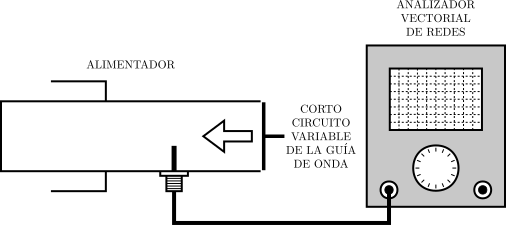
\includegraphics[scale = 1]{Figures/Resultados/resultados_10}
\caption{Banco de medición de la ROE y de la impedancia del alimentador.}
\label{fig_resultados:10}
\end{figure}
%%%%
%%%%
\begin{figure} [H]
\centering 
\includegraphics[scale = 0.3]{Figures/Resultados/resultados_11}
\caption{Cortocircuito variable de la guía de onda.}
\label{fig_resultados:11}
\end{figure}
%%%%
El cortocircuito variable de la guía de onda consiste en un círculo de latón que se va desplazando por el interior de la guía; de esta forma se logra variar la distancia entre el cortocircuito y el excitador, y así se puede minimizar la ROE del alimentador y observar la variación en el VNA. Para asegurarse de que haya buen contacto eléctrico entre la tapa que hace de cortocircuito y la guía de onda, se aplicó grasa conductora de cobre a la pared interior de la guía de onda. También se ajustó la longitud del excitador para minimizar la ROE.
%%%%
\begin{figure}[H]
\centering
\includegraphics[scale = 0.4]{Figures/Resultados/resultados_12}
\caption{Medición de la ROE y de la impedancia del alimentador.}
\label{fig_resultados:12}
\end{figure}
%%%%
En la tabla \ref{tabla_mediciones:1} se comparan las dimensiones del alimentador determinadas por la simulación y la medición.
%%%%
\begin{table}[H]
\centering
\begin{tabular}{|c|c|c|c|}
\hline
Dimensiones & $L_e$ (mm) & $D_c$ (mm) & Longitud del alimentador (mm)\\
\hline
Simulación & 29,2 & 42,3 & 206,0\\
\hline
Medición & 29,1 & 46,3 & 210,0\\
\hline
\end{tabular}
\caption{Comparación entre las dimensiones del alimentador y del excitador determinadas por simulación y medición.}
\label{tabla_mediciones:1}
\end{table}
%%%%
Se muestran a continuación los gráficos de la impedancia y de la ROE medidas, en las figuras \ref{fig_resultados:13}, \ref{fig_resultados:14} y \ref{fig_resultados:15}, para las dimensiones óptimas determinadas experimentalmente, y se comparan con las simulaciones a fin de contrastar los resultados.
%%%%
\begin{figure}[H]
\centering
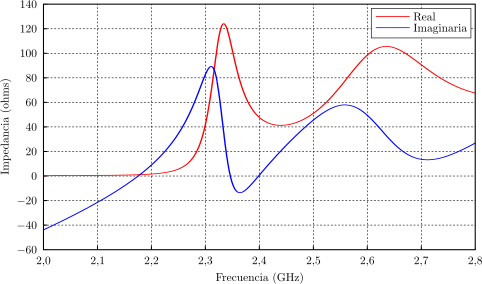
\includegraphics[scale = 1]{Figures/Resultados/resultados_13}
\caption{Simulación de la impedancia del alimentador.}
\label{fig_resultados:13}
\end{figure}
%%%%
%%%%
\begin{figure}[H]
\centering
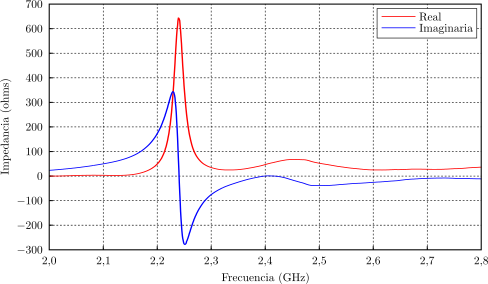
\includegraphics[scale = 1]{Figures/Resultados/resultados_14}
\caption{Medición de la impedancia del alimentador.}
\label{fig_resultados:14}
\end{figure}
%%%%
%%%%
\begin{figure}[H]
\centering
\includegraphics[scale = 1]{Figures/Resultados/resultados_15}
\caption{Simulación y medición de la ROE del alimentador.}
\label{fig_resultados:15}
\end{figure}
%%%%
En la tabla \ref{tabla_mediciones:2} se comparan los valores de impedancia y ROE simulados y medidos del alimentador a la frecuencia de operación, 2,4 GHz. Las incertezas producidas en las mediciones se calcularon en el apéndice \ref{apendice_e}.
%%%%
\begin{table}[H]
\centering
\begin{tabular}{c|c|c|c|}
\cline{2-4}
& \multicolumn{2}{c|}{Impedancia (ohms)} & \multirow{2}{*}{ROE} \\
\cline{2-3}
& Parte real & Parte imaginaria & \\
\hline
\multicolumn{1}{|c|}{Simulación} & 47,72 & 0,75 & 1,05 \\
\hline
\multicolumn{1}{|c|}{Medición} & 47,07 & 0,16 & 1,06 \\
\hline
\end{tabular}
\caption{Comparación entre la simulación y la medición de la impedancia y de la ROE del alimentador.}
\label{tabla_mediciones:2}
\end{table}
%%%%
A partir de los resultados anteriores, se puede observar que los valores obtenidos experimentalmente, tanto para el dimensionamiento del alimentador como para la medición de la impedancia y de la ROE, se aproximan muy bien a los simulados.

Finalmente se ha cortado la guía de onda para que la distancia entre el excitador y el cortocircuito de la guía de onda se ajuste al valor obtenido experimentalmente y se procedió a soldar el cortocircuito definitivo. En la figura \ref{fig_resultados:16} puede observarse el alimentador con el cortocircuito de la guía soldado.
%%%%
\begin{figure}[H]
\centering
\includegraphics[scale = 0.3]{Figures/Resultados/resultados_16}
\caption{Alimentador con el cortocircuito de la guía soldado.}
\label{fig_resultados:16}
\end{figure}
%%%%

%%%%
\section{Medición del diagrama de radiación}
\label{sec_resultados_med_dia_rad}
%%%%

Para medir el diagrama de radiación del alimentador, se implementó el banco de medición de la figura \ref{fig_resultados:17}.
%%%%
\begin{figure}[H]
\centering
\includegraphics[scale = 1]{Figures/Resultados/resultados_17}
\caption{Banco de medición del diagrama de radiación.}
\label{fig_resultados:17}
\end{figure}
%%%%
Se han medido los planos E y H del diagrama de radiación. Como antena patrón se utilizó una bocina piramidal que, según las simulaciones, tiene una ganancia de aproximadamente 12 dBi. Utilizando esta antena de alta ganancia como patrón y colocando ambas antenas a una altura de 1,8 metros se disminuyen los efectos causados por las reflexiones de las ondas electromagnéticas en el recinto de medición. No se ha medido la ganancia del alimentador porque no se cuenta con la infraestructura necesaria. En la figura \ref{fig_resultados:18} puede observarse la bocina piramidal usada como antena patrón.
%%%%
\begin{figure}[H]
\centering
\includegraphics[scale = 0.27]{Figures/Resultados/resultados_18}
\caption{Bocina piramidal empleada como antena patrón.}
\label{fig_resultados:18}
\end{figure}
%%%%
El alimentador se ha instalado sobre un cilindro de madera solidario con el eje de rotación del motor y se ha conectado al analizador de espectros. Para la medición, se ha configurado el analizador de espectros para trabajar con zero span a una frecuencia central de 2,4 GHz. Como el tiempo que el alimentador tarda en dar un giro completo es de aproximadamente 13 segundos, se configuró el barrido del analizador de espectros en 20 segundos para asegurarse que dentro de los valores medidos se tengan dos máximos, que corresponden al instante en que el alimentador esté alineado con la antena patrón.
%%%%
\begin{figure}[H]
\centering
\includegraphics[scale = 0.35]{Figures/Resultados/resultados_19}
\caption{Alimentador instalado sobre el rotador.}
\label{fig_resultados:19}
\end{figure}
%%%%
Para determinar la separación entre la antena patrón y el alimentador, se calculó la distancia de campo lejano; considerando que la máxima dimensión de la antena patrón es de 25 cms, la distancia de campo lejano es:
%%%%
\begin{align*}
D_{cl} = 2\,\dfrac{D^2}{\lambda} = 2\,\dfrac{\left(\text{25 cm}\right)^2}{\text{12,5 cm}} = 1\text{ m}
\end{align*}
%%%%
El banco de medición armado puede observarse en la figura \ref{fig_resultados:20}.
%%%%
\begin{figure}[H]
\centering
\includegraphics[scale = 0.32]{Figures/Resultados/resultados_20}
\caption{Banco de medición implementado.}
\label{fig_resultados:20}
\end{figure}
%%%%
En las figura \ref{grup_fig_resultados:3} pueden observarse las mediciones de los planos E y H del diagrama de radiación, superpuestos a los diagramas de radiación simulados con el fin de poder contrastar mediciones con simulaciones.
%%%%
\begin{figure} [H]
\centering 
\subfigure[Plano E.]{
\label{fig_resultados:21}
\includegraphics[scale = 0.5]{Figures/Resultados/resultados_21}}
\subfigure[Plano H.]{
\label{fig_resultados:22}
\includegraphics[scale = 0.5]{Figures/Resultados/resultados_22}}
\caption{Simulación y medición de los planos E y H del diagrama de radiación del alimentador.}
\label{grup_fig_resultados:3}
\end{figure}
%%%%
Puede notarse que el Plano E del diagrama de radiación medido presenta una asimetría, que se debe a que en el plano en el que se rota el alimentador para realizar la medición se ubica el conector N y la línea de transmisión coaxial, lo que inevitablemente va a afectar la medición. Sin embargo, puede verse que para valores de $\uptheta$ comprendidos entre 0$^{\circ}$ y 90$^{\circ}$ la medición es coincidente con la simulación.

Para la medición del Plano H, dado que el conector N no se ubica en el plano de rotación del alimentador, la condición de simetría es bien marcada, lo que se evidencia en la medición obtenida, que además de ser muy simétrica, es casi coincidente con la simulación.

En la tabla \ref{tabla_mediciones:3} se compara el ancho de haz principal, la ganancia normalizada en el ángulo $\theta_0$ y la relación frente-espalda obtenidos mediante la simulación y la medición. Las incertezas producidas en las mediciones se calcularon en el apéndice \ref{apendice_e}.
%%%%
\begin{table}[H]
\centering
\begin{tabular}{c|c|c|cc|c|}
\cline{2-6}
& \multicolumn{2}{c|}{Ancho de haz} & \multicolumn{2}{c|}{\multirow{2}{*}{$G_{fn}\left(\theta_0\right)\,$(dB)}} & \multirow{2}{*}{Relación frente}\\
& \multicolumn{2}{c|}{principal (grados)} & & & \multirow{2}{*}{espalda (dB)}\\
\cline{2-5}
& Plano E & Plano H & \multicolumn{1}{|c|}{Plano E} & Plano H &\\
\hline
\multicolumn{1}{|c|}{Simulación} & 82,90 & 81,02 & \multicolumn{1}{|c|}{-7,35} & -8,75 & 18,44\\
\hline
\multicolumn{1}{|c|}{Medición} & 82,37 & 85,22 & \multicolumn{1}{|c|}{-7,33} & -8,91 & 17,71\\
\hline
\end{tabular}
\caption{Comparación entre la simulación y la medición del ancho de haz principal, la ganancia normalizada en el ángulo $\theta_0$ y la relación frente-espalda.}
\label{tabla_mediciones:3}
\end{table}
%%%%
Puede observarse que los valores obtenidos experimentalmente son similares a los simulados.


%%%%
\section{Cálculo de las pérdidas óhmicas del alimentador}
\label{sec_resultados_per_ohm_ali}
%%%%

Las pérdidas óhmicas del alimentador dependen tanto de la conductividad del material conductor con el que se construye la antena como de la frecuencia de operación y de las dimensiones de la guía de onda cilíndrica.

Para una guía de onda cilíndrica y considerando el modo de propagación dominante, las pérdidas por unidad de longitud \cite{Balaniselectro} están dadas por:
%%%%
\begin{align*}
\alpha = \dfrac{R_s}{a\eta_0\sqrt{1 - \left(\dfrac{f_c}{f}\right)^2}}\left[\!\left(\dfrac{f_c}{f}\right)^2 \!+ \dfrac{1}{{\chi '_{11}}^2  - 1}\right]\dfrac{\text{Np}}{\text{m}}
\end{align*}
%%%%
donde:
%%%%
\begin{align*}
Rs = \sqrt{\dfrac{\omega\mu}{2\sigma}} =\text{Resistencia superficial.}
\end{align*}
%%%%
Para el diámetro del alimentador, la frecuencia de corte es:
%%%%
\begin{align*}
f_c = \dfrac{c}{2\pi}\dfrac{\chi '_{11}}{a} = \text{2,22 GHz}
\end{align*}
%%%%
y las pérdidas por unidad de longitud:
%%%%
\begin{align*}
\alpha = \text{0,00543}\,\dfrac{\text{Np}}{\text{m}}
\end{align*}
%%%%
Considerando la longitud de la guía de onda y que 1 Np = 8,6858 dB, la atenuación producida en el alimentador resulta:
%%%%
\begin{align*}
AT \simeq \text{0,01 dB}
\end{align*}
%%%%
La atenuación producida es extremadamente baja, por lo que puede considerarse que la ganancia y la directividad del alimentador son iguales.

%%%%
\section{Simulaciones de polarización cruzada}
\label{sec_resultados_sim_pol_cru}
%%%%

En la sección \ref{sec_polarizacion_cruzada} se ha deducido que la máxima polarización cruzada se produce para el plano $\upphi = 45^{\circ}$, por lo que las simulaciones de polarización cruzada se realizaron solamente para ese plano.

En la figura \ref{fig_resultados:23} se observa la simulación de la copolarización y de la polarización cruzada del alimentador.
%%%%
\begin{figure}[H]
\centering
\includegraphics[scale = 1]{Figures/Resultados/resultados_23}
\caption{Simulación de la copolarización y de la polarización cruzada del alimentador para el plano $\upphi = 45^{\circ}$.}
\label{fig_resultados:23}
\end{figure}
%%%%
La relación de polarización cruzada $\rho_L$, cuya expresión es \eqref{ec_intro:78}, según la simulación resulta  $\rho_L$ = 18,63 dB.

En la figura \ref{fig_resultados:24} se observa la simulación de la copolarización y de la polarización cruzada del conjunto formado por el alimentador y el reflector parabólico.
%%%%
\begin{figure}[H]
\centering
\includegraphics[scale = 1]{Figures/Resultados/resultados_24}
\caption{Simulación de la copolarización y de la polarización cruzada del alimentador con el reflector parabólico para el plano $\upphi = 45^{\circ}$.}
\label{fig_resultados:24}
\end{figure}
%%%%
En la figura \ref{fig_resultados:25} puede observarse la simulación de la copolarización y de la polarización cruzada del conjunto formado por el alimentador y el reflector parabólico para valores de $\uptheta$ menores a 15$^{\circ}$, con el fin de observar detalladamente que sucede en la región cercana a la dirección de propagación principal.
%%%%
\begin{figure}[H]
\centering
\includegraphics[scale = 1]{Figures/Resultados/resultados_25}
\caption{Simulación de la copolarización y de la polarización cruzada del alimentador con el reflector parabólico para el plano $\upphi = 45^{\circ}$ (detallada).}
\label{fig_resultados:25}
\end{figure}
%%%%
La relación de polarización cruzada, según la simulación, es 30,85 dB, lo que puede considerarse un resultado muy satisfactorio.

%%%%
\section{Simulaciones de diagramas de radiación}
\label{sec_resultados_sim_dia_rad}
%%%%

En la figura \ref{grup_fig_resultados:4} pueden observarse las simulaciones de los planos E y H del diagrama de radiación del conjunto formado por el alimentador y el reflector parabólico.
%%%%
\begin{figure} [H]
\centering 
\subfigure[Plano E.]{
\label{fig_resultados:26}
\includegraphics[scale = 1]{Figures/Resultados/resultados_26}}
\hspace{5mm}
\subfigure[Plano H.]{
\label{fig_resultados:27}
\includegraphics[scale = 1]{Figures/Resultados/resultados_27}}
\caption{Simulación de los planos E y H del diagrama de radiación del alimentador con el reflector parabólico.}
\label{grup_fig_resultados:4}
\end{figure}
%%%%
La directividad máxima y la eficiencia de abertura determinados a partir de la simulación son:
%%%%
\begin{itemize}
\item Directividad $D_0$: 31,68 dBi.
\item Eficiencia de abertura: 71,93 \%.
\end{itemize}
%%%%
En la tabla \ref{tabla_mediciones:4} se muestra el ancho de haz principal y además el ángulo y la amplitud normalizada del primer lóbulo secundario, según la simulación, en los planos E y H.
%%%%
\begin{table}[H]
\centering
\begin{tabular}{c|c|c|c|}
\cline{2-4}
& Ancho de haz & Ángulo 1.$^{\text{er}}$ lóbulo & Amplitud normalizada 1.$^{\text{er}}$ \\
& principal (grados) & secundario (grados) & lóbulo secundario (dB) \\
\hline
\multicolumn{1}{|c|}{Plano E} & 4,68 & 7,17 & -25,77 \\
\hline
\multicolumn{1}{|c|}{Plano H} & 4,68 & 7,45 & -25,87 \\
\hline
\end{tabular}
\caption{Valores obtenidos por simulación del ancho de haz principal y del ángulo y la amplitud del primer lóbulo secundario en los planos E y H del diagrama de radiación.}
\label{tabla_mediciones:4}
\end{table}
%%%%
Viendo los resultados, tener una eficiencia de abertura superior al 70 \% es un muy buen resultado. Sin embargo, en la práctica existen otros factores que inciden en la eficiencia además de la iluminación del reflector, como las irregularidades en la superficie y la geometría del reflector y los desplazamientos axiales y radiales del alimentador respecto al foco.

Finalmente, en las figuras \ref{fig_resultados:28} y \ref{fig_resultados:29} se observan los diagramas de radiación 3D del alimentador y del alimentador con el reflector parabólico respectivamente.

%%%%
\begin{figure}[H]
\centering
\includegraphics[scale = 0.25]{Figures/Resultados/resultados_28}
\caption{Simulación del diagrama de radiación 3D del alimentador.}
\label{fig_resultados:28}
\end{figure}
%%%%
%%%%
\begin{figure}[H]
\centering
\includegraphics[scale = 0.25]{Figures/Resultados/resultados_29}
\caption{Simulación del diagrama de radiación 3D del alimentador con el reflector parabólico.}
\label{fig_resultados:29}
\end{figure}
%%%%

\chapter{Conclusiones}
\label{cap_conclusiones}
\lhead{Capítulo \ref{cap_conclusiones}. \emph{Conclusiones}}
%%%%%%%%%%%%%%%%
%%  Capítulo 6: Conclusiones  %%
%%%%%%%%%%%%%%%%


El difundido uso de la tecnología \textit{microstrip} suele ser explicado en base a los bajos costos de fabricación que presenta y a la facilidad para la implantación de componentes circuitales discretos. Sin embargo, para las altas frecuencias representa tanto una herramienta como un desafío: la falta de homogeneidad del medio por el que se propagan los campos electromagnéticos, y la consecuente susceptibilidad a la aparición de modos indeseados obligan a que todo análisis cabal que se realice sobre ellas resulte incompleto y en general, complejo. En muchos casos, la disminución del ancho del sustrato dieléctrico interviniente disminuye sustancialmente los efectos de segundo orden, aunque a costa de un resentimiento en la rigidez estructural.

Los sustratos \textit{microstrip} soportan la aparición de ondas de superficie por sus meras características constructivas, dado que presentan una impedancia de superficie reactiva. Estas ondas de superficie pueden ser controladas mediante diversas técnicas, como la efectiva división del sustrato y plano de tierra, las estructuras de plano de tierra degenerado (DGS) y el uso de \enquote{escalones} de permitividad eléctrica en las inmediaciones de los elementos que son fuente de ondas de superficie. En este trabajo se analizó el uso de estructuras EBG para lograr resultados similares. Como estas estructuras surgieron en el campo de la óptica, si bien se parte de conceptos básicos de electromagnetismo, la nomenclatura resulta, por el momento, ambigua, la información se encuentra dispersa y, debido a la relativa novedad de la aplicación de estructuras EBG en microondas, en muchos casos es también contradictoria.

En la mayoría de los casos la obtención de resultados analíticos resulta imposible, por lo que las técnicas de simulación numérica pueden resultar útiles para la predicción del comportamiento de las estructuras \textit{microstrip}. Sin embargo, la relativa complejidad de las mismas genera que las simulaciones de onda completa requieran de mucho tiempo hasta entregar los resultados esperados, por lo que se dificulta su utilización para el diseño. Debe tenerse en cuenta, además, que el diseño de antenas requiere de la consideración de la estructura EBG a utilizar, y que la misma no puede agregarse a radiadores prediseñados, debido a que la modificación del comportamiento de las ondas de superficie genera importantes efectos sobre las características de radiación de la antena.

En este trabajo se presentaron dos alternativas al uso de estas simulaciones de onda completa: el modelado circuital y la utilización de TLM bidimensional. En ninguno de los dos casos, sin embargo, se predijo satisfactoriamente el comportamiento frente a las ondas de superficie: Sólo se modeló el comportamiento ante excitaciones conducidas, en vistas de lograr, a futuro, un modelo que permita comenzar el cálculo a partir del uso de una fuente distribuida sobre los bordes de la estructura. En el caso de la simulación mediante TLM, dado que parte de conceptos intuitivos sencillos, la misma podría resultar una herramienta para la comprensión de los fenómenos más complejos. Sin embargo, dado que la implementación actual se realizó utilizando técnicas de programación ineficientes y un lenguaje de prototipado, los tiempos de simulación no se redujeron lo suficiente, por lo que aun no podrían ser usados en etapas de diseño.

Resulta importante destacar que las ondas de superficie no son la única fuente de acoplamiento y que, en general, no son la más importante. El uso de estructuras EBG debe supeditarse a la relación entre todas las causas de acoplamiento posibles, especialmente debido a que el diseño de estas estructuras es, por el momento, iterativo. La necesidad de iterar en el proceso de diseño, sumado a que las celdas unitarias que ofrecen mejores resultados son también las más complejas, ofrecen muchos grados de libertad y por lo tanto, una mayor cantidad de variables a considerar, dificulta y ralentiza la tarea.

Por otro lado, si bien no se realizaron mediciones para este trabajo, las mismas resultan un paso fundamental para la validación de los resultados analíticos y numéricos obtenidos. La bibliografía y los trabajos de investigadores en los últimos años han demostrado, mediante mediciones, que es posible utilizar estas estructuras para disminuir el acoplamiento mutuo entre antenas que comparten sustrato.

\section{Propuestas de trabajos futuros}

Dado que el presente trabajo representa un primer paso en la comprensión de los fenómenos asociados al funcionamiento de las estructuras EBG, las propuestas de trabajos futuros son muy variadas. En primer lugar, resulta menester intentar aplicar los conceptos de modelado por circuitos de parámetros concentrados para predecir el comportamiento ante la incidencia de ondas de superficie que lo excitan en forma distribuida. Además, para que las simulaciones por TLM resulten efectivamente útiles al momento de diseñar, es necesario volcar los conceptos a un lenguaje de programación tipado y más eficiente que Python. Finalmente, el diseño completo de un conjunto de antenas, y no el meramente ilustrativo aplicado en este trabajo, para probar, mediante simulaciones y, principalmente, mediciones, el funcionamiento de estas estructuras, permitiría avanzar sobre terreno más firme en el uso de EBGs con estos fines.

Por otro lado, además de las geometrías analizadas, en los últimos años han surgido diversas estructuras que permiten efectos multibanda, a partir de lograr una controlada variación geometría de las celdas unitarias, como se analiza en \cite{Kern:multiband}. Por otro lado, resulta importante lograr efectos similares utilizando celdas unitarias más pequeñas, de modo que se pueda ubicar una mayor cantidad de celdas entre las antenas involucradas. Entre las distintas propuestas analizadas, resultan destacables las que utilizan curvas de Peano y de Hilbert para lograr una mayor inductancia el menor área posible, como se analiza en \cite{McVay:Peano}. Estos EBGs, que presentan un ancho de banda mayor, disminuyen la presión sobre el diseñador, quien puede utilizar la misma estructura aunque la frecuencia de trabajo varíe.

Podría resultar interesante, además, analizar posibles aplicaciones de las celdas complementarias a las propuestas, donde las porciones que no poseen cobre y las que sí, son intercambiadas, dado que poseen la misma periodicidad que las celdas originales. El uso de celdas complementarias resulta común en el estudio de \textit{Frequency Selective Surfaces} (FSS).

Otras técnicas para controlar la propagación de ondas de superficie han sido propuestas, entre las que destaca el uso de planos de tierra degenerados (DGS, \textit{degenerated ground planes}), que son muy similares a los EBGs. El principio de funcionamiento es el mismo, pero el hecho de que se estructuren geometrías sobre el plano de tierra modifica genera efectos sobre la radiación posterior.

Además de las ondas de superficie, que pueden ser atenuadas por los EBGs, existe también acoplamiento debido a modos cuasi-TEM que viajan por encima del sustrato, como una onda libre, y que no pueden ser bloqueados por las estructuras propuestas. Si se busca un desacoplamiento más notorio, es importante reducir el aporte de las mismas. Estudios en este sentido pueden consultarse en \cite{Asimonis:designoptimization}.


%%%%

%%%%

\clearpage\pagestyle{empty}\mbox{}\clearpage  % Página en blanco.


%%  ------------------------------------------------------------------------------------  %%
%% 			 Aquí comienzan los apéndices, incluyéndolos como archivos separados 	   	  %%
%%  ------------------------------------------------------------------------------------  %%


\appendix  % Para incluir los apéndices.
\clearpage
\addappheadtotoc  % Agrega la página con la leyenda "Apéndices" al índice.
\appendixpage  % Agrega una página con la leyenda "Apéndices".

\chapter{Distribución de los campos en una cinta microstrip}
\label{apendice_a}
\lhead{Apéndice \ref{apendice_a}. \emph{Distribución de los campos en una cinta microstrip}}
Una onda electromagnética incidente sobre una superficie en un ángulo arbitrario puede analizarse descomponiendo el problema en dos casos canónicos de polarización\footnote{La polarización es la dirección del campo eléctrico. En nuestro análisis, se considera polarización lineal, de modo que el campo eléctrico en distintos puntos del espacio siempre puede ser representado por vectores colineales.}: perpendicular (TE, transversal eléctrico) o paralela (TM, transversal magnético) al plano de incidencia, que es el formado por el rayo incidente y la normal a la interfaz. El problema de la incidencia perpendicular a la interfaz combina ambos casos.

\begin{figure} [H]
	\centering 
	\subfigure[Polarización paralela (TM).]{
		\label{fig:oblique_incidence_parallel}
		\includegraphics[width=0.45\textwidth]{intro_electro/incidencia_oblicua_paralela-version2.pdf}}
	\hspace{5mm}
	\subfigure[Polarización perpendicular (TE).]{
		\label{fig:oblique_incidence_perp}
		\includegraphics[width=0.45\textwidth]{intro_electro/incidencia_oblicua_perpendicular-version2.pdf}}
	\caption{Incidencia oblicua para los dos casos de polarización analizados.}
	\label{fig:oblique_incidence}
\end{figure}

Los campos eléctrico y magnético incidentes, según el sistema de coordenadas definido en la Figura \ref{fig:oblique_incidence}, pueden ser expresados, en forma general, usando las expresiones \ref{eq:electric_field_wave_solution} y \ref{eq:relacion-e-h-ondaplana}, y considerando que no hay pérdidas, como indican las ecuaciones \ref{eq:incident_fields}:

\begin{align}
	\label{eq:incident_fields}
	\vec{E}_i &= \vec{E}_0 \;e^{-j\vec{\beta}_1 \cdot \vec{r}} &
	\vec{H}_i = \frac{\hat{\beta}_1 \times \vec{E}_0}{\eta_1} \;e^{-j\vec{\beta}_1 \cdot \vec{r}}
\end{align}

donde $\vec{r}=(x,y,z)$, $\vec{\beta}_1 = \hat{\beta}_1 \;\omega \sqrt{\mu_1 \epsilon_1}$. $\hat{\beta}_1$ es la dirección de propagación de la onda plana, y $\eta_1 = \sqrt{\mu_1 / \epsilon_1} = j\omega \mu / \gamma$ es la impedancia de onda de región de incidencia.

Se define al coeficiente de reflexión $\Gamma$ como la relación entre la magnitud del campo reflejado y del campo incidente, $E_r / E_i$. De la misma manera, el coeficiente de transmisión $T$ es la relación entre el módulo del campo transmitido al segundo medio y el campo incidente desde el primer medio, $E_t / E_i$, de manera que $1+\Gamma = T$ y que $(1-\Gamma)/\eta_1 = T/\eta_2$. 

Usando estos coeficientes, a partir de las ecuaciones \ref{eq:incident_fields}, y teniendo en cuenta las condiciones de borde descriptas en la Sección \ref{sec:condiciones-borde}, se pueden calcular los campos reflejados y transmitidos. Para los dos casos canónicos analizados, los campos incidentes, reflejados y transmitidos se resumen en la tabla \ref{table:incidencia_oblicua}, así como los coeficientes de reflexión y transmisión.

\tabulinesep=1.2mm
\taburulecolor{black!20}
\begin{table}
	
	\begin{tabu} to 1\textwidth {gX[c]@{}X[c]@{}}
		\rowcolor{black!20} & \multicolumn{1}{c}{\textbf{TM}} & \multicolumn{1}{c}{\textbf{TE}}\\
		$\vec{E}_i$
		&
		\scalebox{0.86}{%
			$
			E_0\; (\hat{z}\; \mathrm{cos}\; \theta_i + \hat{x}\; \mathrm{sin}\; \theta_i)\; e^{-j \beta_1 (z\; \mathrm{sin}\; \theta_i - x\; \mathrm{cos}\; \theta_i)}
			$
		}	
		&
		\scalebox{0.86}{%
			$
			E_0\; \hat{y} \;e^{-j \beta_1 (z\; \mathrm{sin}\; \theta_i - x\; \mathrm{cos}\; \theta_i)}
			$
		} \\
		$\vec{H}_i$
		&
		\scalebox{0.86}{%
			$
			\frac{E_0}{\eta_1}\; \hat{y}\; e^{-j \beta_1 (z\; \mathrm{sin}\; \theta_i - x\; \mathrm{cos}\; \theta_i)}
			$
		}
		&
		\scalebox{0.86}{%
			$
			\frac{E_0}{\eta_1} \;(-\hat{z}\; \mathrm{cos}\; \theta_i - \hat{x}\; \mathrm{sin}\; \theta_i)\; e^{-j \beta_1 (z\; \mathrm{sin}\; \theta_i - x\; \mathrm{cos}\; \theta_i)}
			$
		} \\
		\hline
	
		$\vec{E}_r$
		&
		\scalebox{0.86}{%
			$
			E_0\; \Gamma\; (\hat{z}\; \mathrm{cos}\; \theta_r - \hat{x}\; \mathrm{cos}\; \theta_r)\; e^{-j \beta_1 (x\; \mathrm{sin}\; \theta_r + z\; \mathrm{sin}\; \theta_r)}
			$
		}	
		&
		\scalebox{0.86}{%
			$
			E_0\; \Gamma\; \hat{y} \;e^{-j \beta_1 (z\; \mathrm{sin}\; \theta_r + x\; \mathrm{cos}\; \theta_r)}
			$
		} \\
		$\vec{H}_r$
		&
		\scalebox{0.86}{%
			$
			-\frac{E_0\; \Gamma}{\eta_1}\; \hat{y}\; e^{-j \beta_1 (x\; \mathrm{sin}\; \theta_r + z\; \mathrm{sin}\; \theta_r)}
			$
		}
		&
		\scalebox{0.86}{%
			$
	 		\frac{E_0\; \Gamma}{\eta_1} \;(\hat{z}\; \mathrm{cos}\; \theta_r - \hat{x}\; \mathrm{sin}\; \theta_r)\; e^{-j \beta_1 (z\; \mathrm{sin}\; \theta_r + x\; \mathrm{cos}\; \theta_r)}
			$
		} \\
	\hline
		$\vec{E}_t$
		&
		\scalebox{0.86}{%
			$
			E_0\; T\; (\hat{z}\; \mathrm{cos}\; \theta_t + \hat{x}\; \mathrm{sin}\; \theta_t) e^{-j \beta_2 (z\; \mathrm{sin}\; \theta_t - x\; \mathrm{cos}\; \theta_t)}
			$
		}
		&
		\scalebox{0.86}{%
			$
			E_0\; T\; \hat{y}\; e^{-j \beta_2 (z\; \mathrm{sin}\; \theta_t - x\; \mathrm{cos}\; \theta_t)}
			$
		} \\
		$\vec{H}_t$
		&
		\scalebox{0.86}{%
			$
	 		\frac{E_0\; T}{\eta_1}\; \hat{y}\; e^{-j \beta_2 (z\; \mathrm{sin}\; \theta_t - x\; \mathrm{cos}\; \theta_t)}
			$
		}
		&
		\scalebox{0.86}{%
			$
			\frac{E_0\; T}{\eta_2}\; (-\hat{z}\; \mathrm{cos}\; \theta_t - \hat{x}\; \mathrm{sin}\; \theta_t)\; e^{-j \beta_2 (z\; \mathrm{sin}\; \theta_t - x\; \mathrm{cos}\; \theta_t)}
			$
		} \\
		\hline
		
		$\Gamma$
		&
		$\frac{\eta_2\; \cos\; \theta_t - \eta_1 \; \cos\; \theta_i}{\eta_2\; \cos\; \theta_t + \eta_1 \; \cos\; \theta_i}$
		&
		$\frac{\eta_2\; \cos\; \theta_i - \eta_1 \; \cos\; \theta_t}{\eta_2\; \cos\; \theta_i + \eta_1 \; \cos\; \theta_t}$
		\\
		$T$
		&
		$\frac{2 \;\eta_2 \; \cos\; \theta_i}{\eta_2\; \cos\; \theta_t + \eta_1 \; \cos\; \theta_i}$
		&
		$\frac{2\; \eta_2 \; \cos\; \theta_i}{\eta_2\; \cos\; \theta_i + \eta_1 \; \cos\; \theta_t}$
	\end{tabu}
	\caption{Campos incidentes, transmitidos y reflejados, y coeficientes de reflexión y transmisión para incidencia oblicua de una onda plana sobre una interfaz dieléctrica.}
	\label{table:incidencia_oblicua}
\end{table}

Si se fuerza la continuidad de las componentes tangenciales de los campos sobre la interfaz para ambos casos, $\vec{E}_i^{tg} + \vec{E}_r^{tg} = \vec{E}_t^{tg}$ y $\vec{H}_i^{tg} + \vec{H}_r^{tg} = \vec{H}_t^{tg}$, se obtienen las expresiones \ref{eq:continuidad_campos_paralelo} para el modo TM, y \ref{eq:continuidad_campos_perpendicular} para el modo TE.

\begin{equation}
	\begin{aligned}
		cos \; \theta_i \; e^{-j \beta_1 z \sin \; \theta_i} + \Gamma \; cos \; \theta_r \; e^{-j \beta_1 z \; \sin\; \theta_r} &= T\; \cos\; \theta_t \; e^{-j \beta_2 z \; \sin\; \theta_t}\\
		\frac{1}{\eta_1} \; e^{-j \beta_1 z \; \sin \theta_i} - \frac{\Gamma}{\eta_1} \; e^{-j \beta_1 z \; \sin \; \theta_r} &= \frac{T}{\eta_2} \; e^{-j \beta_2 z \; \sin\; \theta_t}
	\end{aligned}
	\label{eq:continuidad_campos_paralelo}
\end{equation}

\begin{equation}
	\begin{aligned}
		e^{-j \beta_1 z \sin \; \theta_i} + \Gamma \; e^{-j \beta_1 z \; \sin\; \theta_r} &= T\; e^{-j \beta_2 z \; \sin\; \theta_t}\\
		-\frac{1}{\eta_1} \cos\; \theta_i \; e^{-j \beta_1 z \; \sin \theta_i} - \frac{\Gamma}{\eta_1} \; \cos\; \theta_r e^{-j \beta_1 z \; \sin \; \theta_r} &= -\frac{T}{\eta_2} \; \cos\; \theta_t \; e^{-j \beta_2 z \; \sin\; \theta_t}
	\end{aligned}
	\label{eq:continuidad_campos_perpendicular}
\end{equation}

En estas ecuaciones se observa que a ambos lados de las igualdades, las expresiones son funciones de la posición sobre la interfaz. Para que la condición de borde se cumpla en todos sus puntos, la variación en $z$ debe ser la misma en todos los términos, de forma que el efecto de la variación sea anulado: $\beta_1 \; \sin\; \theta_i = \beta_1 \; \sin \; \theta_r = \beta_2 \; \sin\; \theta_t$.  De esta consideración se deriva la Ley de Snell (asumiendo que $\mu_1 = \mu_2$), expresada en la ecuación \ref{eq:snell_law}. En la gráfica de la Figura \ref{fig:ley_snell} se puede observar el comportamiento del ángulo de refracción según en ángulo de incidencia, sobre una interfaz entre aire y FR4, en sentidos opuestos.

\begin{subequations}
	\label{eq:snell_law}
	\begin{align}x
	\theta_i &= \theta_r\\
	\beta_1 \; \sin\; \theta_i = \beta_2 \; \sin\; \theta_t & \overset{\eta=\omega\mu/\beta}{\Longrightarrow} \eta_2 \; \sin\; \theta_i = \eta_1 \; \sin\; \theta_t  \label{eq:snell_law_second}
	\end{align}
\end{subequations}

\begin{figure}[htp]
	\centering
	\includegraphics[width=0.7\textwidth]{intro_electro/angulo-refraccion-snell.pdf}
	\caption{Ángulo de refracción en función del ángulo de incidencia, según la ley de Snell.}
	\label{fig:ley_snell}
\end{figure}

Utilizando estas expresiones, y a partir de las ecuaciones \ref{eq:continuidad_campos_paralelo} y \ref{eq:continuidad_campos_perpendicular}, se obtienen las expresiones para los coeficientes de reflexión y transmisión de la tabla \ref{table:incidencia_oblicua}. Resulta importante destacar que, para el caso de incidencia perpendicular ($\theta_i = 0$), los coeficientes quedan simplificados a $\Gamma = (\eta_2 - \eta_1)/(\eta_2 + \eta_1)$ y $T = (2 \; \eta_2)/(\eta_2 + \eta_1)$.

Los coeficientes de transmisión y reflexión para incidencia oblicua, en ambas polarizaciones, se pueden graficar en función del ángulo incidente, teniendo en cuenta las ecuaciones de Snell para expresar el ángulo de transmisión en función del ángulo de incidencia. Estas gráficas se muestran, para la interfaz aire-FR4, en la Figura \ref{fig:coeficientes-aire-fr4}, donde, además,  teniendo en cuenta la constante de propagación compleja de la ecuación \ref{eq:constante-propagacion-compleja}, se graficó también el caso con pérdidas, donde se observa, en general, una mayor reflexión y, por tanto, menor transmisión. Para ángulos de incidencia rasantes, la transmisión es mínima y la reflexión es máxima.

Resulta ilustrativo, además, graficar el comportamiento según el ángulo de incidencia de la misma interfaz, pero en el sentido dieléctrico-aire. Este gráfico se observa en la Figura \ref{fig:coeficientes-fr4-aire}, donde los coeficientes de transmisión pueden ser mayores a 1 porque el ángulo en el segundo medio es menor al de incidencia, permitiendo conservar el flujo de energía por unidad de área.

\begin{figure}[H]
	\centering 
	\subfigure[Coeficiente de reflexión entre aire y FR4 en función de $\theta_i$.]{
		\label{fig:coeficiente-reflexion-aire-fr4}
		\includegraphics[width=0.48\textwidth]{intro_electro/plot-comparacion-lossy-lossless-annotated.pdf}}
	\subfigure[Coeficiente de transmisión entre aire y FR4 en función de $\theta_i$.]{
		\label{fig:coeficiente-transmision-aire-fr4}
		\includegraphics[width=0.48\textwidth]{intro_electro/plot-comparacion-lossy-lossless-T.pdf}}
	\caption{Coeficientes de transmisión y reflexión para el caso en que el medio de incidencia es aire, y el medio de transmisión es FR4.}
	\label{fig:coeficientes-aire-fr4}
\end{figure}


\begin{figure}[htp]
	\centering
	\includegraphics[width=0.7\textwidth]{intro_electro/plot-coeficientes-fresnel-dirInversa.pdf}
	\caption{Comportamiento de los coeficientes de reflexión y transmisión para el caso de incidencia FR4-aire.}
	\label{fig:coeficientes-fr4-aire}
\end{figure}



\section{Ángulo de Brewster y ángulo crítico}

Se conoce como ángulo de Brewster al ángulo de incidencia $\theta_i$ necesario para que se produzca reflexión nula ($\Gamma = 0$) en una interfaz, cuando sobre ella incide una onda plana en forma oblicua. Este efecto se da únicamente para la polarización TM, es decir, cuando existe componente de campo eléctrico en la dirección normal a la interfaz, por lo que suele ser utilizado como mecanismo para lograr polarización de una onda electromagnética.

Si se anulan los coeficientes de reflexión mostrados en la tabla \ref{table:incidencia_oblicua}, y se utilizan las ecuaciones \ref{eq:snell_law}, se puede deducir que la polarización TE no presenta ángulo de Brewster\footnote{Para lograr reflexión nula en TE se requiere que $\sin \; \theta_i / \sin \; \theta_t = cos \; \theta_i / cos \; \theta_t = \eta_1 / \eta_2$, lo cual es imposible.}, aunque sí lo hace la polarización TM\footnote{Para lograr reflexión nula en TM se requiere que $\sin \; \theta_i / \sin \; \theta_t = cos \; \theta_t / cos \; \theta_i = \eta_1 / \eta_2$, lo cual no supone una contradicción. Multiplicando la ecuación \ref{eq:snell_law_second} y el valor de $\Gamma$ para polarización TM, se obtiene que $\sin\;\theta_i \; cos \; \theta_i = \sin \; \theta_t \; cos \; \theta_t$, ó $\sin \; 2\theta_i = \sin \; 2\theta_t$, que se satisface cuando $2\theta_i = \pi - 2\theta_t$, de modo que $\theta_i + \theta_t = \pi/2$.}, cuando $\theta_i + \theta_t = \pi/2$. Aplicando esta condición en la Ley de Snell (ecuación \ref{eq:snell_law_second}) se obtiene la expresión del ángulo de Brewster:

%%% GRAFICAR LO DE ACA ARRIBA, REEMPLAZANDO THETA_T POR LA LEY DE SNELL. EJE X: THETA_I. DE ESTA MANERA SE PODRIA VERIFICAR QUE PARA TE NO HAY SOLUCION Y PARA TM SI.

\begin{align}
	\label{eq:Brewster_angle}
	\tan\;\theta_B &= \frac{\eta_1}{\eta_2} = \sqrt{\frac{\epsilon_2}{\epsilon_1}}
\end{align}

Como se observa en la Figura \ref{fig:Brewster-funcion-epsilon}, el ángulo de Brewster tiende a $90^{\circ}$ cuando la permeabilidad eléctrica del segundo medio es mucho mayor a la del primero, lo que significa que para evitar reflexiones, el ángulo de incidencia debe ser rasante. Cuando se da el caso contrario, en que la permeabilidad eléctrica del medio incidente es mayor a la del medio de transmisión, el ángulo de Brewster se vuelve menor a $45^{\circ}$, de lo que se deduce que una incidencia \textit{casi} perpendicular a la interfaz, y en consecuencia con polarización \textit{cercana} a TEM (aunque no exactamente TEM) lograría evitar la reflexión. El ángulo de $45^{\circ}$ cuando las permeabilidades eléctricas de ambos medios son iguales es meramente anecdótico, ya que si no existen diferencias entre los dos medios que forman la interfaz, la misma no existe, y por lo tanto no hay onda reflejada para \textit{ningún} ángulo de incidencia.

\begin{figure} [H]
	\centering 
	\subfigure[Ángulo de Brewster en función de $\epsilon_2/\epsilon_1$.]{
		\label{fig:Brewster-funcion-epsilon}
		\includegraphics[width=0.48\textwidth]{intro_electro/plot-brewster.pdf}}
	\subfigure[Ángulo crítico y rango de reflexión total en función de $\epsilon_2/\epsilon_1$.]{
		\label{fig:angulo-critico-funcion-epsilon}
		\includegraphics[width=0.48\textwidth]{intro_electro/plot-angulo-critico.pdf}}
	\caption{}
	\label{fig:angulo-critico-epsilon}
\end{figure}

En la figura  \ref{fig:coeficientes-aire-fr4} se puede observar el comportamiento de los coeficientes de reflexión y transmisión alrededor del ángulo de Brewster para polarización TM, cuando no se consideran pérdidas. Para polarización TE, el ángulo de Brewster no existe, y una situación similar se da cuando existen pérdidas en los materiales, incluso para polarización TM. En la Figura \ref{fig:coeficientes-fr4-aire} también se puede observar el fenómeno de ángulo de Brewster, aunque debido a la dirección de la onda incidente, el mismo es mucho menor.


En ángulo crítico se define como el ángulo de incidencia para el cual la onda incidente es totalmente reflejada, y la onda transmitida no se propaga a la segunda región.

Si se observan las expresiones del coeficiente de transmisión de la tabla \ref{table:incidencia_oblicua}, el único valor de $\theta_i$ para el cual la transmisión es nula es $\pi/2$, es decir, incidencia rasante. Sin embargo, a partir de la ecuación \ref{eq:snell_law_second}, se obtiene que $\sin \; \theta_t = \eta_2 / \eta_1\; \sin\; \theta_i$. Se puede observar que en los casos en que $\eta_2 > \eta_1$ es posible que el ángulo de transmisión alcance el valor $\pi/2$ antes de que lo haga en ángulo de incidencia. El ángulo crítico, entonces, surge de la expresión \ref{eq:angulo_critico}, graficada en la Figura \ref{fig:angulo-critico-epsilon}. En la gráfica se puede observar que si $\epsilon_2 = \epsilon_1$, el único ángulo para el que hay reflexión completa es el rasante. A medida que disminuye la relación entre las permeabilidades dieléctricas, el valor del ángulo crítico disminuye, hasta que el valor de la permitividad dieléctrica del segundo medio es mucho mayor a la del primero, lo que vuelve a las impedancias de onda muy disimiles, generando que haya reflexión total para cualquier ángulo de incidencia.

\begin{equation}
	\label{eq:angulo_critico}
	\sin\; \theta_i^c = \frac{\eta_1}{\eta_2}\;\sin \; \theta_t|_{\theta_t=\pi/2} = \sqrt{\frac{\epsilon_2}{\epsilon_1}} \implies \theta_c = \arcsin \;\sqrt{\frac{\epsilon_2}{\epsilon_1}} = \arcsin \;\frac{\eta_1}{\eta_2}
\end{equation}

Para ángulos mayores a $\theta_c$, las expresiones del coeficiente de reflexión se vuelven complejas y de módulo 1, por lo que toda la energía electromagnética es reflejada, y la onda transmitida tiene un comportamiento evanescente, como se muestra en la Figura \ref{fig:angulo_critico}. En la ecuación \ref{eq:angulo_critico} se observa que si $\theta_i > \theta_c$, el ángulo $\theta_t$ pierde significado físico, debido a que $\sin\; \theta_t$ debería ser mayor a 1 para cumplir la ecuación.

\begin{figure}[htp]
	\centering
	\includegraphics[width=0.6\textwidth]{intro_electro/angulo_critico.pdf}
	\caption{Ilustración del comportamiento de una onda plana durante la incidencia con ángulo critico y con ángulo mayor al $\theta_c$.}
	\label{fig:angulo_critico}
\end{figure}

Se debe notar que en el argumento anterior no se consideró la polarización de la onda incidente, por lo que la reflexión completa se puede dar tanto en modo TM como en modo TE, siempre y cuando la incidencia se produzca desde el medio ópticamente más denso al menos denso \cite{Fernandez:Electromag}, como se muestra en la Figura \ref{fig:coeficientes-fr4-aire}. Sin embargo, resulta útil expresar el comportamiento de los campos.

Para el caso de una onda incidente con una polarización lineal arbitraria como la expresada en la ecuación \ref{eq:incident_fields}, se debe considerar que la componente longitudinal a la interfaz del vector de onda $\vec{\gamma}$ se mantendrá constante, de modo que $\gamma_{2_z} = \gamma_{1_z} = \gamma_1 \; \sin \; \theta_i$. La componente transversal a la interfaz, en cambio, será $\gamma_{2_x} = \gamma_2\; \cos \; \theta_t = \gamma_2 \sqrt{1-sin^2\theta_t} = \gamma_{2_x}$. Dado que para el caso en que el ángulo incidente es mayor al ángulo crítico se requiere que $\sin\;\theta_t > 1$, el valor de ${\gamma_2}_x$ será imaginario, $-i\alpha$ \footnote{El signo negativo se desprende de la imposibilidad física de un crecimiento exponencial del valor del campo, lo cual descarga la posibilidad de que el signo sea positivo}. De esta forma, para direcciones de campos arbitrarias, y teniendo en cuenta el hecho de que el vector $\vec{\gamma}$ se desarrolla sobre el plano de incidencia:

\begin{subequations}
	\begin{align}
		\vec{E}_t (\vec{r},t) = \vec{E}_2 \; e^{-j \vec{\gamma}_2 \cdot \vec{r}} = \vec{E}_2 \; e^{-j({\gamma_2}_x x + {\gamma_2}_z z)} = \vec{E}_2 \; e^{-j(\beta z - j\alpha x)} = \vec{E}_2 \; e^{-j\beta z} \; e^{- \alpha x}\\
		\vec{H}_t (\vec{r},t) = \vec{H}_2 \; e^{-j \vec{\gamma}_2 \cdot \vec{r}} = \vec{H}_2 \; e^{-j({\gamma_2}_x x + {\gamma_2}_z z)} = \vec{H}_2 \; e^{-j(\beta z - j\alpha x)} = \vec{H}_2 \; e^{-j\beta z} \; e^{- \alpha x}
	\end{align}
\end{subequations}

Se observa que en la dirección perpendicular a la interfaz hay un comportamiento evanescente o exponencial decreciente de la onda transmitida, mientras que existe propagación en la dirección paralela a la interfaz, dando lugar a lo que se conoce como onda de superficie.

La ecuación del módulo del vector de onda (\ref{eq:numero_de_onda}) resulta redefinida como $\beta_x^2 - \alpha_z^2 = \gamma_2^2$, de donde se deduce que $\alpha_z = \sqrt{\gamma_x^2\;sin^2\;\theta_i - \gamma_2^2}$. % Distribución de los campos en guías de ondas

\chapter{Cálculo del diagrama de dispersión}
\label{apendice_b}
\lhead{Apéndice \ref{apendice_b}. \emph{Cálculo del diagrama de dispersión}}
Para poder utilizar las técnicas de blindaje contra ondas de superficie utilizando metamateriales, como las descriptas en el informe, es necesario que el ancho de la banda prohibida de la estructura EBG resulte mayor al ancho de banda de la antena. Es debido al alto valor del factor Q (y por tanto, bajo ancho de banda) de las antenas \textit{microstrip} rectangulares el motivo por el que el uso de estructuras EBG es factible.
La caracterización del comportamiento de las estructuras de banda prohibida electromagnética ubicadas entre antenas \textit{microstrip} para frecuencias más allá de la de resonancia escapa del objetivo de este trabajo. Sin embargo, el tema se trató repetidas veces durante el desarrollo del trabajo, especialmente debido a que se debió considerar la viabilidad de realizar mediciones de caracterización del EBG para realizar comparaciones con las simulaciones obtenidas. Este apéndice pretende introducir conceptualmente el tema.

Existen numerosas técnicas que permiten aumentar el ancho de banda de las estructuras radiantes de tecnología \textit{microstrip}. Como se explicó antes, una técnica común consiste en aumentar al ancho del sustrato, o cambiarlo por otro de constante dieléctrica menor. Debido a que la modificación de cualquiera de los dos parámetros condicionaría sustancialmente el comportamiento de las ondas de superficie generadas sobre el sustrato, se decidió que resultaba importante independizarlos del análisis.

En otros casos, se ha propuesto la modificación de la geometría del elemento radiante, descartando el tradicional parche rectangular por figuras con formas de U o de E, o por formas geométricas con aperturas radiantes embebidas \cite{Yang:EBGAntennas}. Para las mediciones de este trabajo se consideró, y finalmente se descartó, el uso de antenas \textit{microstrip} de tipo moño (\textit{bow-tie}), que presentan una transición geométrica suave, intuitivamente apta para las necesidades presentadas. Entre las dificultades que ofrece, está su principio de funcionamiento, comparable al de un dipolo, y requiriendo, por tanto, una alimentación en modo diferencial, lo que obligaría a realizar un diseño de un balún \textit{microstrip}, lejano a las pretensiones del trabajo.

Otra técnica común consiste en diseñar conjuntos de elementos que resuenan a distintas y frecuencias, acoplados capacitivamente, denominados estructuras multi-resonantes. Si las distintas frecuencias de resonancia están lo suficientemente cerca unas de otras, se logra un efecto de continuidad, aumentando notoriamente el ancho de banda. En muchos casos, y debido a los costos cada vez más despreciables de la fabricación de circuitos multicapa, los elementos resonantes se ubican apilados, generando un acoplamiento capacitivo máximo entre ellos. Para el caso de las pruebas que se requieren hacer para validar y caracterizar el comportamiento de las estructuras EBG, elementos radiantes coplanares con el parche activo resonante resultan suficientes.

La estructura propuesta consiste en un parche rectangular, ubicado sobre un sustrato de FR4, de comportamiento resonante en una frecuencia aproximada de 2.4 GHz, y ubicado entre dos rectángulos \textit{microstrip} pasivos iguales, de un largo establecido de forma que la frecuencia de resonancia de los mismos resulte ligeramente diferente a la del parche activo. La distancia entre estos elementos de carga y la antena original debe ser tal que el acoplamiento sea notorio, requisito que presenta complejidades \cite{Kumar:radiating} debido a que los parches deben estar ubicados frente a los bordes no radiantes de la antena para evitar reducir el espacio utilizado por la estructura EBG con la que compartirán sustrato. En la figura \ref{fig:antena-propuesta-con-ebg} se puede observar el arreglo final de elementos. Se debe destacar que la elección de que ambos parches posean las mismas propiedades geométricas se debe a la búsqueda de la máxima simetría par para simplificar el análisis de la estructura, aún cuando esta elección merme la flexibilidad del diseño de banda ancha.

\begin{figure}[h]
	\centering
	\includegraphics[width=0.9\textwidth]{Aplicacion/estructura-antenas-ebg.pdf}
	\caption{Estructura propuesta para la caracterización del efecto de EBGs sobre antenas microstrip.}
	\label{fig:antena-propuesta-con-ebg}
\end{figure}


Los parches rectangulares, al igual que en el desarrollo del análisis de estructuras EBG, están acoplados al elemento activo mediante lo que puede modelarse como una red $\pi$ de capacitores (acoplamiento capacitivo) \cite{Kumar:Non-radiating}, similar a mostrada en la figura \ref{fig:acoplamiento-capacitivo-modelo}, donde los denominados \textit{pixeles} deben ser reemplazados por los parches propiamente dichos. En términos generales, los parámetros que modificarán la impedancia de entrada y que, por lo tanto, afectarán al ancho de banda, son la distancia entre el resonador activo y los pasivos ($g'$), la longitud de los parches acoplados ($l'$) y la posición del punto de alimentación \cite{Kumar:Non-radiating}.

La existencia de estos parches, que pueden considerarse como de carga, implican una modificación de la impedancia de entrada para distintas frecuencias.

Si los parches pasivos poseen dimensiones muy disímiles al parche activo central, las frecuencias de resonancia de los elementos estarán tan alejadas entre sí que es posible un análisis simplificado del comportamiento: A bajas frecuencias, los rectángulo pasivos no resuenan ni se acoplan visiblemente al parche activo. A medida que la frecuencia de trabajo aumenta, los mismos comienzan a acoplarse, adoptando un comportamiento capacitivo, al mismo tiempo que debido a que forman un paralelo con la carga impuesta por la resistencia de radiación, disminuyen el valor de la resistencia de entrada. Una vez que los parches resuenan, logrando que se presente la mínima resistencia de entrada, obtienen un comportamiento de carácter inductivo, hasta que nuevamente, a altas frecuencias, dejan de tener injerencia palpable sobre el valor de la impedancia de entrada. La variación de la distancia entre los parches da lugar a que estos efectos se vuelvan más o menos plausibles, en función del acoplamiento capacitivo \cite{Kumar:Non-radiating}.

Cuando los parches pasivos poseen geometrías similares a la del parche original, el problema resulta más complejo, debido a que no puede analizarse la resonancia de cada elemento por separado sin considerar la carga que los demás ejercen sobre él. Debido a que, a fin de aumentar el ancho de banda, todos los parches deberán tener geometrías similares, resulta necesario realizar simulaciones numéricas que permitan predecir el comportamiento.

Para observar el efecto del uso de parches \textit{microstrip} acoplados capacitivamente al parche activo principal para aumentar el ancho de banda del sistema radiante, se realizaron sucesivas simulaciones en el software de simulación CST Microwave Studio, realizando una optimización para obtener el mayor ancho de banda posible dentro del rango de interés. Los parches deben ser de un largo similar a la antena, aunque ligeramente diferente, para aumentar el ancho de banda. Por otro lado, se eligió que fueran simétricos, a fin de no aumentar la anisotropía del problema.

Resulta conveniente, en este caso, realizar simulaciones para comprender el efecto de la variación de distintos parámetros, en particular de la distancia entre el radiador activo y los parches, $g'$, el ancho $w'$ de los parches y su largo $l'$. Las primeras simulaciones, utilizando los valores obtenidos en el análisis de un parche único, demostraron que los parches de carga efectivamente cambian las frecuencia de resonancia. 

En la figura \ref{fig:unparche-concarga-sinebg-varAnchoLprima} se puede observar el comportamiento, para distintos valores de $l'$, con $w'$ y $g'$ fijos, habiendo elegido los valores del parche óptimos obtenidos antes (donde se consideró un parche sin carga). Se observa que para todos los valores de $l'$ probados, la frecuencia de resonancia del sistema, o la frecuencia para la que el parámetro $S_{11}$ es mínima, disminuye notablemente, debido al acoplamiento entre elementos y la aparición de modos de menor frecuencia. En todas las curvas se observan dos mínimos locales. Cuando las cargas tienen un largo $l'$ menor al de la antena \textit{microstrip}, como es el caso para 25 mm y 28.75 mm, existe un mínimo a una frecuencia superior a la buscada, que para el caso de 25 mm queda fuera de la gráfica. De la misma manera, cuando el largo de las cargas es mayor al del parche, se presenta un mínimo a una frecuencia inferior. Como se explicó antes, el caso óptimo se da cuando ambos mínimos coinciden o están lo suficientemente cerca en frecuencia para aumentar el ancho de banda del sistema radiante. Se observa, también, que el mínimo absoluto del parámetro $S_{11}$ adopta un valor menor, más deseable, para valores de $l'$ por debajo de $L$, mientras que se ubica en una posición más cercana a la frecuencia buscada para valores por encima de $L$. Esta última variación podría controlarse mediante la disminución del tamaño de la geometría completa.

En la figura \ref{fig:unparche-concarga-sinebg-varDistanciaCarga} se puede observar que una mayor distancia entre el parche \textit{microstrip} y las cargas da lugar a una frecuencia de resonancia menor. Sin embargo, el mínimo local cercano a 2.17 GHz generado por la presencia de los parches de carga no varía notoriamente con la distancia. Por otro lado, el valor que adopta el mínimo absoluto parece ser menor cuando la distancia es pequeña.

Finalmente, en la figura \ref{fig:unparche-concarga-sinebg-varAltoWprima} se muestra la variación del comportamiento en frecuencia del parámetro $S_{11}$ en función de la variación del ancho $w'$ de los parches carga. La frecuencia donde se ubica el mínimo absoluto es mayor cuando el parche carga es angosto, ya que limita la formación de modos indeseados.

\begin{figure}[H]
	\centering 
	\subfigure[Variación del largo $l'$.]{
		\label{fig:unparche-concarga-sinebg-varAnchoLprima}
		\includegraphics[width=0.47\textwidth]{Aplicacion/VariacionAnchoLprima-UnParcheConCarga.pdf}}
	\subfigure[Variación de la distancia entre la carga y el parche, $g'$.]{
		\label{fig:unparche-concarga-sinebg-varDistanciaCarga}
		\includegraphics[width=0.47\textwidth]{Aplicacion/VariacionDistanciagprimera-UnParcheConCarga.pdf}}
	\subfigure[Variación de valor de $w'$.]{
		\label{fig:unparche-concarga-sinebg-varAltoWprima}
		\includegraphics[width=0.50\textwidth]{Aplicacion/VariacionAltowprima-UnParcheConCarga.pdf}}
	\caption{Variación del parámetro $S_{11}$ del puerto en función de distintos parámetros del parche único, y antena optimizada final.}
	\label{fig:simulaciones-microstrip-1parchecargado}
\end{figure}

% Analizar por qué pasan cosas raras.
% Poner foto del diseño del único parche cargado final.
	% Expresiones de los campos radiados por aberturas rectangulares

\chapter{Algoritmo de TLM modificado}
\label{apendice_c}
\lhead{Apéndice \ref{apendice_c}. \emph{Algoritmo de TLM modificado}}
%\newlength{\longitudNtheta}
%\settowidth{\longitudNtheta}{$N_{\theta}$}
%%\the\longitudNtheta\\
%\newlength{\longitudNphi}
%\settowidth{\longitudNphi}{$N_{\phi}$}
%%\the\longitudNphi\\
%\newlength{\longitudLtheta}
%\settowidth{\longitudLtheta}{$L_{\theta}$}
%%\the\longitudLtheta\\
%\newlength{\longitudLphi}
%\settowidth{\longitudLphi}{$L_{\phi}$}
%%\the\longitudLphi\\
%\newlength{\longitudEtheta}
%\settowidth{\longitudEtheta}{$E_{\theta}$}
%%\the\longitudEtheta\\
%\newlength{\longitudEphi}
%\settowidth{\longitudEphi}{$E_{\phi}$}
%%\the\longitudEphi\\
%\newlength{\longitudEthetanor}
%\settowidth{\longitudEthetanor}{$\lvert E_{\theta}^{\circ}\left(\theta,\phi\right)\rvert^2$}
%%\the\longitudEthetanor\\
%\newlength{\longitudEphinor}
%\settowidth{\longitudEphinor}{$\lvert E_{\phi}^{\circ}\left(\theta,\phi\right)\rvert^2$}
%%\the\longitudEphinor\\

%%%%
\section{Abertura circular con plano conductor infinito y excitación con campo uniforme}
\label{subsec_apendice_c_abert_circ_inf_uni}
%%%%

%%%%
Los campos sobre la abertura están dados por:
%%%%
\begin{align}
\mathbf{E}_a &= 
\begin{cases}
\makebox[0pt][l]{$E_0\,\versor{y}$}\hphantom{-E_0\,\versor{x}} &\text{si } \rho' \leq a\\
0  &\text{caso contrario}
\end{cases}
\label{ec_apC:1}\\
\mathbf{H}_a &= 
\begin{cases} 
-E_0\,\versor{x} &\text{si } \rho' \leq a\\
0  & \text{caso contrario}
\end{cases}
\label{ec_apC:2}
\end{align}
%%%%
Empleando el modelo equivalente de la Figura \ref{fig_fundamentos:8}, las densidades de corriente quedan expresadas como:
%%%%
\begin{align}
\mathbf{M}_s &=
\begin{cases}
2E_0\,\versor{x} &\text{si } \rho' \leq a\\
0 &\text{caso contrario}
\end{cases}
\label{ec_apC:3}\\
\mathbf{J}_s &= \makebox[0pt][l]{$0$} 
\hphantom{\begin{cases} 2E_0\,\versor{x}\\0\end{cases}}\kern-\nulldelimiterspace
\forall\,x',y'
\label{ec_apC:4}
\end{align}
%%%%
Considerando que:
%%%%
\begin{subequations}
\label{grup_ec_apC:1}
\begin{align}
M_\rho  &= M_x\cos\phi '
\label{ec_apC:5}\\
M_\phi &= -M_x\sen\phi '
\label{ec_apC:6}
\end{align}
\end{subequations}
%%%%
las expresiones \eqref{grup_ec_fundamentos:6} resultan:
%%%%
\begin{subequations}
\label{grup_ec_apC:2}
\begin{align}
N_{\theta} &= 0
\label{ec_apC:7}\\
N_{\phi} &= 0
\label{ec_apC:8}\\
L_{\theta}  &= 2E_0\cos\theta\cos\phi\!\int_{0}^{\,a}\!\rho '\,d\rho '\!\int_{0}^{\,2\pi}\!e^{jk\rho '\sen\theta\cos\left(\phi - \phi '\right)}\,d\phi '
\label{ec_apC:9}\\
L_{\phi} &= -2E_0\sen\phi\!\int_{0}^{\,a}\!\rho '\,d\rho '\!\int_{0}^{\,2\pi}\!e^{jk\rho '\sen\theta\cos\left(\phi - \phi '\right)}\,d\phi '
\label{ec_apC:10}
\end{align}
\end{subequations}
%%%%
A partir de la integral definida \cite{walfram_bessel_first}:
%%%%
\begin{align}
\int_{0}^{\,2\pi}\!e^{jz\cos\left(\phi - \phi '\right)}\,d\phi ' = 2\pi J_0\!\left(z\right)
\label{ec_apC:11}
\end{align}
%%%%
las expresiones \eqref{ec_apC:9} y \eqref{ec_apC:10} se reducen a:
%%%%
\begin{subequations}
\label{grup_ec_apC:3}
\begin{align}
L_{\theta} &= 4\pi E_0\cos\theta\cos\phi\!\int_{0}^{\,a}\!\rho 'J_0\!\left(k\rho '\sen\theta\right)d\rho '
\label{ec_apC:12}\\
L_{\phi} &= - 4\pi E_0\sen\phi\!\int_{0}^{\,a}\!\rho 'J_0\!\left(k\rho '\sen\theta\right)d\rho '
\label{ec_apC:13}
\end{align}
\end{subequations}
%%%%
donde $J_0\!\left(z\right)$ es la Función de Bessel de primera especie y orden cero.

Realizando el reemplazo de variables:
%%%%
\begin{align}
t = k\rho '\sen\theta\Longrightarrow dt = k\sen\theta\, d\rho '
\label{ec_apC:14}
\end{align}
%%%%
$L_{\theta}$ y $L_{\phi}$ se expresan como:
%%%%
\begin{subequations}
\label{grup_ec_apC:4}
\begin{align}
L_{\theta} &= 4\pi E_0\frac{\cos\theta\cos\phi}{\left(k\sen\theta\right)^2}\!\int_{0}^{\,ka\sen\theta}\!tJ_0\!\left(t\right)dt
\label{ec_apC:15}\\
L_{\phi} &= - 4\pi E_0\frac{\sen\phi}{\left(k\sen\theta\right)^2}\!\int_{0}^{\,ka\sen\theta}\!tJ_0\!\left(t\right)dt
\label{ec_apC:16}
\end{align}
\end{subequations}
%%%%
Utilizando la propiedad \cite{walfram_bessel_first}:
%%%%
\begin{align}
\int_{0}^{\,\beta}\!zJ_0\!\left(z\right)dz = \beta J_1\!\left(\beta\right)
\label{ec_apC:17}
\end{align}
%%%%
las expresiones \eqref{grup_ec_apC:4} se reducen a:
%%%%
\begin{subequations}
\label{grup_ec_apC:5}
\begin{align}
L_{\theta} &= 4\pi a^2E_0\!\left[\cos\theta\cos\phi\left(\frac{J_1\!\left(ka\sen\theta\right)}{ka\sen\theta}\right)\right]
\label{ec_apC:18}\\
L_{\phi} &= - 4\pi a^2E_0\!\left[\sen\phi\left(\frac{J_1\!\left(ka\sen\theta\right)}{ka\sen\theta}\right)\right]
\label{ec_apC:19}
\end{align}
\end{subequations}
%%%%
donde $J_1\!\left(z\right)$ es la Función de Bessel de primera especie y orden uno.

Introduciendo las expresiones \eqref{grup_ec_apC:5}, los campos radiados por la abertura \eqref{grup_ec_fundamentos:3} pueden expresarse como:
%%%%
\begin{subequations}
\label{grup_ec_apC:6}
\begin{align}
E_r &\simeq 0
\label{ec_apC:20}\\
E_\theta &\simeq j\frac{a^2kE_0e^{-jkr}}{r}\left[\sen\phi\left(\frac{J_1\!\left(ka\sen\theta\right)}{ka\sen\theta}\right)\right]
\label{ec_apC:21}\\
E_\phi &\simeq j\frac{a^2kE_0e^{-jkr}}{r}\left[\cos\theta\cos\phi\left(\frac{J_1\!\left(ka\sen\theta\right)}{ka\sen\theta}\right)\right]
\label{ec_apC:22}\\
H_r &\simeq 0
\label{ec_apC:23}\\
H_\theta &\simeq -\frac{E_\phi}{\eta}
\label{ec_apC:24}\\
H_\phi &\simeq +\frac{E_\theta}{\eta}
\label{ec_apC:25}
\end{align}
\end{subequations}
%%%%
Para hallar la intensidad de radiación a partir de la expresión \eqref{ec_intro:15}, primero se determina $\lvert E_{\theta}^{\circ}\left(\theta,\phi\right)\rvert^2$ y $\lvert E_{\phi}^{\circ}\left(\theta,\phi\right)\rvert^2$, cuyas expresiones son:
%%%%
\begin{subequations}
\label{grup_ec_apC:7}
\begin{align}
\lvert E_{\theta}^{\circ}\left(\theta,\phi\right)\rvert^2 &= \frac{a^4k^2\left|E_0\right|^2}{r^2}\sen^2\phi\left(\frac{J_1\!\left(ka\sen\theta\right)}{ka\sen\theta}\right)^2
\label{ec_apC:26}\\
\lvert E_{\phi}^{\circ}\left(\theta,\phi\right)\rvert^2 &= \frac{a^4k^2\left|E_0\right|^2}{r^2}\cos^2\theta\cos^2\phi\left(\frac{J_1\!\left(ka\sen\theta\right)}{ka\sen\theta}\right)^2
\label{ec_apC:27}
\end{align}
\end{subequations}
%%%%
La expresión de la intensidad de radiación resulta:
%%%%
\begin{align}
U = \frac{a^4k^2\left|E_0\right|^2}{2\eta}\left(\sen^2\phi + \cos^2\theta\cos^2\phi \right)\!\left(\frac{J_1\!\left(ka\sen\theta\right)}{ka\sen\theta}\right)^2
\label{ec_apC:28}
\end{align}
%%%%
De la expresión \eqref{ec_apC:28} se obtiene el factor de diagrama de potencia $F\left(\theta,\phi\right)$ y la constante $B_0$, por lo que:
%%%%
\begin{gather}
F\left(\theta,\phi\right) = \left(\sen^2\phi + \cos^2\theta\cos^2\phi \right)\!\left(\frac{J_1\!\left(ka\sen\theta\right)}{ka\sen\theta}\right)^2
\label{ec_apC:29}\\
B_0 = \frac{a^4k^2\left|E_0\right|^2}{2\eta}
\label{ec_apC:30}
\end{gather}
%%%%
La directividad se calcula a partir de la expresión \eqref{ec_intro:18}, empleando el factor de diagrama de potencia determinado en la expresión \eqref{ec_apC:29}.
%%%%

%%%%
\section{Abertura circular con plano conductor infinito y excitación con campo sinusoidal en modo dominante}
\label{subsec_apendice_c_abert_circ_inf_dom}
%%%%

%%%%
A partir de las componentes transversales de los campos en una guía de onda cilíndrica para modo dominante, cuyas expresiones son \eqref{grup_ec_apA:29}, se deduce que los campos sobre la abertura están dados por:
%%%%
\begin{align}
\mathbf{E}_a &= 
\begin{cases} 
\makebox[0pt][l]{$E_0\,\dfrac{\sen\phi '}{\rho '}\,J_1\!\left(\dfrac{\chi '_{11}}{a}\rho '\right)\!\versor{\uprho} + E_0\cos\phi '\,{J_1}'\!\left(\dfrac{\chi '_{11}}{a}\rho '\right)\!\versor{\upphi}$}\hphantom{- \dfrac{E_0}{\eta}\cos\phi '\,{J_1}'\!\left(\dfrac{\chi '_{11}}{a}\rho '\right)\!\versor{\uprho} + \dfrac{E_0}{\eta}\dfrac{\sen\phi '}{\rho '}\,J_1\!\left(\dfrac{\chi '_{11}}{a}\rho '\right)\!\versor{\upphi}} &\text{si } \rho '\leq a\\
0 &\text{caso contrario}
\end{cases}
\label{ec_apC:31}\\
\mathbf{H}_a &= 
\begin{cases} 
- \dfrac{E_0}{\eta}\cos\phi '\,{J_1}'\!\left(\dfrac{\chi '_{11}}{a}\rho '\right)\!\versor{\uprho} + \dfrac{E_0}{\eta}\dfrac{\sen\phi '}{\rho '}\,J_1\!\left(\dfrac{\chi '_{11}}{a}\rho '\right)\!\versor{\upphi} &\text{si } \rho '\leq a\\
0  &\text{caso contrario}
\end{cases}
\label{ec_apC:32}
\end{align}
%%%%
Empleando el modelo equivalente de la Figura \ref{fig_fundamentos:9}, las densidades de corriente quedan expresadas como:
%%%%
\begin{align}
\mathbf{M}_s &=
\begin{cases}
2E_0\cos\phi '\,{J_1}'\!\left(\dfrac{\chi '_{11}}{a}\rho '\right)\!\versor{\uprho} - 2E_0\,\dfrac{\sen\phi '}{\rho '}\,J_1\!\left(\dfrac{\chi '_{11}}{a}\rho '\right)\!\versor{\upphi} &\text{si } \rho ' \leq a\\
0 &\text{caso contrario}
\end{cases}
\label{ec_apC:33}\\
\mathbf{J}_s &= \makebox[0pt][l]{$0$} 
\hphantom{\begin{cases}2E_0\cos\phi '\,{J_1}'\!\left(\dfrac{\chi '_{11}}{a}\rho '\right)\!\versor{\uprho} - 2E_0\,\dfrac{\sen\phi '}{\rho '}\,J_1\!\left(\dfrac{\chi '_{11}}{a}\rho '\right)\!\versor{\upphi}\\0\end{cases}}\kern-\nulldelimiterspace
\forall\,x',y'
\label{ec_apC:34}
\end{align}
%%%%
y las expresiones \eqref{grup_ec_fundamentos:6} como:
%%%%
\begin{subequations}
\label{grup_ec_apC:8}
\begin{align}
N_{\theta} &= 0
\label{ec_apC:35}\\
N_{\phi} &= 0
\label{ec_apC:36}\\
L_{\theta}  &= 2E_0\cos\theta\left\{\int_{0}^{\,a}\!\rho '{J_1}'\!\left(\frac{\chi '_{11}}{a}\rho '\right)\!\left[\int_{0}^{\,2\pi}\!\cos\phi '\cos\left(\phi - \phi '\right)e^{jk\rho '\sen\theta\cos\left(\phi - \phi '\right)}\,d\phi '\right]\!d\rho '\right.\notag\\
&\left.-\int_{0}^{\,a}J_1\!\left(\frac{\chi '_{11}}{a}\rho '\right)\!\left[\int_{0}^{\,2\pi}\!\sen\phi '\sen\left(\phi - \phi '\right)e^{jk\rho '\sen\theta\cos\left(\phi - \phi '\right)}\,d\phi '\right]\!d\rho '\right\}
\label{ec_apC:37}\\
L_{\phi} &= - 2E_0\left\{\int_{0}^{\,a}\!\rho '{J_1}'\!\left(\frac{\chi '_{11}}{a}\rho '\right)\!\left[\int_{0}^{\,2\pi}\!\cos\phi '\sen\left(\phi - \phi '\right)e^{jk\rho '\sen\theta\cos\left(\phi - \phi '\right)}\,d\phi '\right]\!d\rho '\right.\notag\\
&\left.+\int_{0}^{\,a}J_1\!\left(\frac{\chi '_{11}}{a}\rho '\right)\!\left[\int_{0}^{\,2\pi}\!\sen\phi '\cos\left(\phi - \phi '\right)e^{jk\rho '\sen\theta\cos\left(\phi - \phi '\right)}\,d\phi '\right]\!d\rho '\right\}
\label{ec_apC:38}
\end{align}
\end{subequations}
%%%%
A partir de las integrales definidas \cite{walfram_bessel_first}:
%%%%
\begin{subequations}
\label{grup_ec_apC:9}
\begin{align}
\int_{0}^{\,2\pi}\!\cos\phi '\cos\left(\phi - \phi '\right)e^{jz\cos\left(\phi - \phi '\right)}\,d\phi ' &= \pi\cos\phi\left[J_0\!\left(z\right) - J_2\!\left(z\right)\right]
\label{ec_apC:39}\\
\int_{0}^{\,2\pi}\!\sen\phi '\sen\left(\phi - \phi '\right)e^{jz\cos\left(\phi - \phi '\right)}\,d\phi ' &= -\pi\cos\phi\left[J_0\!\left(z\right) + J_2\!\left(z\right)\right]
\label{ec_apC:40}\\
\int_{0}^{\,2\pi}\!\cos\phi '\sen\left(\phi - \phi '\right)e^{jz\cos\left(\phi - \phi '\right)}\,d\phi ' &= \pi\sen\phi\left[J_0\!\left(z\right) + J_2\!\left(z\right)\right]
\label{ec_apC:41}\\
\int_{0}^{\,2\pi}\!\sen\phi '\cos\left(\phi - \phi '\right)e^{jz\cos\left(\phi - \phi '\right)}\,d\phi ' &= \pi\sen\phi\left[J_0\!\left(z\right) - J_2\!\left(z\right)\right]
\label{ec_apC:42}
\end{align}
\end{subequations}
%%%%
las expresiones \eqref{ec_apC:37} y \eqref{ec_apC:38} se reducen a:
%%%%
\begin{subequations}
\label{grup_ec_apC:10}
\begin{align}
\begin{split}
L_{\theta}  &= 2\pi E_0\cos\theta\cos\phi\left\{\int_{0}^{\,a}\!\rho '{J_1}'\!\left(\frac{\chi '_{11}}{a}\rho '\right)\!\left[J_0\!\left(k\rho '\sen\theta\right) - J_2\!\left(k\rho '\sen\theta\right)\right]\!d\rho '\right.\\
&\left.+\int_{0}^{\,a}\!J_1\!\left(\frac{\chi '_{11}}{a}\rho '\right)\!\left[J_0\!\left(k\rho '\sen\theta\right) + J_2\!\left(k\rho '\sen\theta\right)\right]d\rho '\right\}
\end{split}
\label{ec_apC:43}\\
\begin{split}
L_{\phi} &= - 2\pi E_0\sen\phi\left\{\int_{0}^{\,a}\!\rho '{J_1}'\!\left(\frac{\chi '_{11}}{a}\rho '\right)\!\left[J_0\!\left(k\rho '\sen\theta\right) + J_2\!\left(k\rho '\sen\theta\right)\right]\!d\rho '\right.\\
&\left.+\int_{0}^{\,a}\!J_1\!\left(\frac{\chi '_{11}}{a}\rho '\right)\!\left[J_0\!\left(k\rho '\sen\theta\right) - J_2\!\left(k\rho '\sen\theta\right)\right]d\rho '\right\}
\end{split}
\label{ec_apC:44}
\end{align}
\end{subequations}
%%%%
Empleando las relaciones de recurrencia de las funciones de Bessel \cite{walfram_bessel_first}:
%%%%
\begin{align}
\frac{n}{z}J_n\!\left(z\right) &= \frac{1}{2}\left[J_{n - 1}\!\left(z\right) + J_{n + 1}\!\left(z\right)\right]
\label{ec_apC:45}\\
{J_n}'\!\left(z\right) &= \frac{1}{2}\left[J_{n - 1}\!\left(z\right) - J_{n + 1}\!\left(z\right)\right]
\label{ec_apC:46}
\end{align}
%%%%
se llega a las expresiones:
%%%%
\begin{align}
{J_1}'\!\left(z\right) + \frac{J_1\!\left(z\right)}{z} &= J_0\!\left(z\right)
\label{ec_apC:47}\\
{J_1}'\!\left(z\right) - \frac{J_1\!\left(z\right)}{z} &= -J_2\!\left(z\right)
\label{ec_apC:48}
\end{align}
%%%%
por lo que $L_{\theta}$ y $L_{\phi}$ se expresan como:
%%%%
\begin{subequations}
\label{grup_ec_apC:11}
\begin{align}
\begin{split}
L_{\theta} &= 2\pi\frac{\chi '_{11}}{a}E_0\cos\theta\cos\phi\left[\int_{0}^{\,a}\!\rho 'J_0\!\left(\frac{\chi '_{11}}{a}\rho '\right)\!J_0\!\left(k\rho '\sen\theta\right)d\rho '\right.\\
&+\left.\int_{0}^{\,a}\!\rho 'J_2\!\left(\frac{\chi '_{11}}{a}\rho '\right)\!J_2\!\left(k\rho '\sen\theta\right)d\rho '\right]
\end{split}
\label{ec_apC:49}\\
\begin{split}
L_{\phi} &= - 2\pi\frac{\chi '_{11}}{a}E_0\sen\phi\left[\int_{0}^{\,a}\!\rho 'J_0\!\left(\frac{\chi '_{11}}{a}\rho '\right)\!J_0\!\left(k\rho '\sen\theta\right)d\rho '\right.\\
&-\left.\int_{0}^{\,a}\!\rho 'J_2\!\left(\frac{\chi '_{11}}{a}\rho '\right)\!J_2\!\left(k\rho '\sen\theta\right)d\rho '\right]
\end{split}
\label{ec_apC:50}
\end{align}
\end{subequations}
%%%%
Utilizando la fórmula integral de Lommel \cite{walfram_bessel_first}:
%%%%
\begin{align}
&\int_{0}^{\,z}\!zJ_n\!\left(\alpha z\right)\!J_n\!\left(\beta z\right)dz = \frac{z}{\alpha^2 - \beta^2}\left[J_n\!\left(\alpha z\right)\!{J_n}'\!\left(\beta z\right) - {J_n}'\!\left(\alpha z\right)\!J_n\!\left(\beta z\right)\right]
\label{ec_apC:51}
\end{align}
%%%%
es posible definir las integrales:
%%%%
\begin{subequations}
\label{grup_ec_apC:12}
\begin{align}
\int_{0}^{\,a}\!\rho 'J_0\!\left(\alpha\rho '\right)\!J_0\!\left(\beta\rho '\right)d\rho ' &= \frac{a}{\alpha^2 - \beta^2}\left[\alpha J_0\!\left(\beta a\right)\!J_1\!\left(\alpha a\right) - \beta J_0\!\left(\alpha a\right)\!J_1\!\left(\beta a\right)\right]
\label{ec_apC:52}\\
\int_{0}^{\,a}\!\rho 'J_2\!\left(\alpha\rho '\right)\!J_2\!\left(\beta\rho '\right)d\rho ' &= \frac{a}{\alpha^2 - \beta^2}\left[\beta J_1\!\left(\beta a\right)\!J_2\!\left(\alpha a\right) - \alpha J_1\!\left(\alpha a\right)\!J_2\!\left(\beta a\right)\right]
\label{ec_apC:53}
\end{align}
\end{subequations}
%%%%
Sumando y restando las integrales \eqref{grup_ec_apC:12}, se obtiene:
%%%%
\begin{subequations}
\label{grup_ec_apC:13}
\begin{align}
\int_{0}^{\,a}\!\rho '\!\left[J_0\!\left(\alpha\rho '\right)\!J_0\!\left(\beta\rho '\right) + J_2\!\left(\alpha\rho '\right)\!J_2\!\left(\beta\rho '\right)\right]d\rho ' &= \frac{2\alpha a}{\alpha^2 - \beta^2}J_1\!\left(\alpha a\right)\!{J_1}'\!\left(\beta a\right)
\label{ec_apC:54}\\
\int_{0}^{\,a}\!\rho '\!\left[J_0\!\left(\alpha\rho '\right)\!J_0\!\left(\beta\rho '\right) - J_2\!\left(\alpha\rho '\right)\!J_2\!\left(\beta\rho '\right)\right]d\rho ' &= \frac{2}{\alpha \beta}J_1\!\left(\alpha a\right)\!J_1\!\left(\beta a\right)
\label{ec_apC:55}
\end{align}
\end{subequations}
%%%%
y a partir de las expresiones \eqref{grup_ec_apC:13}, las expresiones \eqref{grup_ec_apC:11} se reducen a:
%%%%
\begin{subequations}
\label{grup_ec_apC:14}
\begin{align}
&\hspace{\longitudLphi}\hspace{-\longitudLtheta}\raisebox{3.46mm}{$L_{\theta} = 4\pi aJ_1\!\left(\chi_{11}'\right)\!E_0$}\!\left[\raisebox{3.46mm}{$\cos\theta\cos\phi$}\left(\raisebox{3.46mm}{$\dfrac{{J_1}'\!\left(ka\sen\theta\right)}{1 - \left(\dfrac{ka\sen\theta}{\chi_{11}'}\right)^2}$}\right)\!\right]
\label{ec_apC:56}\\
&L_{\phi}  = -4\pi aJ_1\!\left(\chi_{11}'\right)\!E_0\!\left[\sen\phi\left(\dfrac{J_1\!\left(ka\sen\theta\right)}{ka\sen\theta}\right)\right]
\label{ec_apC:57}
\end{align}
\end{subequations}
%%%%
Introduciendo las expresiones \eqref{grup_ec_apC:14}, los campos radiados por la abertura \eqref{grup_ec_fundamentos:3} pueden expresarse como:
%%%%
\begin{subequations}
\label{grup_ec_apC:15}
\begin{align}
E_r &\simeq 0
\label{ec_apC:58}\\
E_{\theta} &\simeq j\frac{aJ_1\!\left(\chi_{11}'\right)\!kE_0e^{-jkr}}{r}\!\left[\sen\phi\left(\dfrac{J_1\!\left(ka\sen\theta\right)}{ka\sen\theta}\right)\right]
\label{ec_apC:59}\\
&\hspace{-\longitudEphi}\raisebox{3.46mm}{$E_{\phi} \simeq j\dfrac{aJ_1\!\left(\chi_{11}'\right)\!kE_0e^{-jkr}}{r}$}\!\left[\raisebox{3.46mm}{$\cos\theta\cos\phi$}\left(\raisebox{3.46mm}{$\dfrac{{J_1}'\!\left(ka\sen\theta\right)}{1 - \left(\dfrac{ka\sen\theta}{\chi_{11}'}\right)^2}$}\right)\!\right]
\label{ec_apC:60}\\
H_r &\simeq 0
\label{ec_apC:61}\\
H_\theta &\simeq -\frac{E_\phi}{\eta}
\label{ec_apC:62}\\
H_\phi &\simeq +\frac{E_\theta}{\eta}
\label{ec_apC:63}
\end{align}
\end{subequations}
%%%%
Para hallar la intensidad de radiación a partir de la expresión \eqref{ec_intro:15}, primero se determina $\lvert E_{\theta}^{\circ}\left(\theta,\phi\right)\rvert^2$ y $\lvert E_{\phi}^{\circ}\left(\theta,\phi\right)\vert^2$, cuyas expresiones son:
%%%%
\begin{subequations}
\label{grup_ec_apC:16}
\begin{align}
&\hspace{\longitudEphinor}\hspace{-\longitudEthetanor}\lvert E_{\theta}^{\circ}\left(\theta,\phi\right)\rvert^2 = \dfrac{a^2\left[J_1\!\left(\chi_{11}'\right)\right]^2k^2\left|E_0\right|^2}{r^2}\sen^2\phi\left(\dfrac{J_1\!\left(ka\sen\theta\right)}{ka\sen\theta}\right)^2
\label{ec_apC:64}\\
&\raisebox{3.46mm}{$\lvert E_{\phi}^{\circ}\left(\theta,\phi\right)\rvert^2 = \dfrac{a^2\left[J_1\!\left(\chi_{11}'\right)\right]^2k^2\left|E_0\right|^2}{r^2}$}\,\raisebox{3.46mm}{$\cos^2\theta\cos^2\phi$}\left(\raisebox{3.46mm}{$\dfrac{{J_1}'\!\left(ka\sen\theta\right)}{1 - \left(\dfrac{ka\sen\theta}{\chi_{11}'}\right)^2}$}\right)^{\!2}
\label{ec_apC:65}
\end{align}
\end{subequations}
%%%%
La expresión de la intensidad de radiación resulta:
%%%%
\begin{align}
\raisebox{3.46mm}{$U = \dfrac{a^2\left[J_1\!\left(\chi_{11}'\right)\right]^2k^2\left|E_0\right|^2}{2\eta}$}\!\left[\raisebox{3.46mm}{$\sen^2\phi\left(\dfrac{J_1\!\left(ka\sen\theta\right)}{ka\sen\theta}\right)^2 \!\!+ \cos^2\theta\cos^2\phi  $}\left(\raisebox{3.46mm}{$\dfrac{{J_1}'\!\left(ka\sen\theta\right)}{1 - \left(\dfrac{ka\sen\theta}{\chi_{11}'}\right)^2}$}\right)^{\!2}\,\right]
\label{ec_apC:66}
\end{align}
%%%%
De la expresión \eqref{ec_apC:66} se obtiene el factor de diagrama de potencia $F\left(\theta,\phi\right)$ y la constante $B_0$, por lo que:
%%%%
\begin{gather}
\raisebox{3.46mm}{$F\left(\theta,\phi\right) =\sen^2\phi\left(\dfrac{J_1\!\left(ka\sen\theta\right)}{ka\sen\theta}\right)^2 \!\!+ \cos^2\theta\cos^2\phi$}\left(\raisebox{3.46mm}{$\dfrac{{J_1}'\!\left(ka\sen\theta\right)}{1 - \left(\dfrac{ka\sen\theta}{\chi_{11}'}\right)^2}$}\right)^{\!2}
\label{ec_apC:67}\\
B_0 = \dfrac{a^2\left[J_1\!\left(\chi_{11}'\right)\right]^2k^2\left|E_0\right|^2}{2\eta}
\label{ec_apC:68}
\end{gather}
%%%%
La directividad se calcula a partir de la expresión \eqref{ec_intro:18}, empleando el factor de diagrama de potencia determinado en la expresión \eqref{ec_apC:67}.
%%%%

%%%%
\section{Guía de onda cilíndrica con extremo abierto}
\label{subsec_apendice_c_guia_cili}
%%%%

%%%%
A partir de las componentes transversales de los campos en una guía de onda cilíndrica para modo dominante, cuyas expresiones son \eqref{grup_ec_apA:29}, se deduce que los campos sobre la abertura están dados por:
%%%%
\begin{align}
\mathbf{E}_a &= 
\begin{cases} 
\makebox[0pt][l]{$E_0\,\dfrac{\sen\phi '}{\rho '}\,J_1\!\left(\dfrac{\chi '_{11}}{a}\rho '\right)\!\versor{\uprho} + E_0\cos\phi '\,{J_1}'\!\left(\dfrac{\chi '_{11}}{a}\rho '\right)\!\versor{\upphi}$}\hphantom{- \dfrac{E_0}{\eta}\cos\phi '\,{J_1}'\!\left(\dfrac{\chi '_{11}}{a}\rho '\right)\!\versor{\uprho} + \dfrac{E_0}{\eta}\dfrac{\sen\phi '}{\rho '}\,J_1\!\left(\dfrac{\chi '_{11}}{a}\rho '\right)\!\versor{\upphi}} &\text{si } \rho '\leq a\\
0 &\text{caso contrario}
\end{cases}
\label{ec_apC:69}\\
\mathbf{H}_a &= 
\begin{cases} 
- \dfrac{E_0}{\eta}\cos\phi '\,{J_1}'\!\left(\dfrac{\chi '_{11}}{a}\rho '\right)\!\versor{\uprho} + \dfrac{E_0}{\eta}\dfrac{\sen\phi '}{\rho '}\,J_1\!\left(\dfrac{\chi '_{11}}{a}\rho '\right)\!\versor{\upphi} &\text{si } \rho '\leq a\\
0  &\text{caso contrario}
\end{cases}
\label{ec_apC:70}
\end{align}
%%%%
Empleando el modelo equivalente de la Figura \ref{fig_fundamentos:10}, las densidades de corriente quedan expresadas como:
%%%%
\begin{align}
\mathbf{M}_s &=
\begin{cases}
\makebox[0pt][l]{$E_0\cos\phi '\,{J_1}'\!\left(\dfrac{\chi '_{11}}{a}\rho '\right)\!\versor{\uprho} - E_0\,\dfrac{\sen\phi '}{\rho '}\,J_1\!\left(\dfrac{\chi '_{11}}{a}\rho '\right)\!\versor{\upphi}$}\hphantom{- \dfrac{E_0}{\eta}\cos\phi '\,{J_1}'\!\left(\dfrac{\chi '_{11}}{a}\rho '\right)\!\versor{\upphi} - \dfrac{E_0}{\eta}\,\dfrac{\sen\phi '}{\rho '}\,J_1\!\left(\dfrac{\chi '_{11}}{a}\rho '\right)\!\versor{\uprho}} &\text{si } \rho '\leq a\\
0 &\text{caso contrario}
\end{cases}
\label{ec_apC:71}\\
\mathbf{J}_s &= 
\begin{cases} 
- \dfrac{E_0}{\eta}\cos\phi '\,{J_1}'\!\left(\dfrac{\chi '_{11}}{a}\rho '\right)\!\versor{\upphi} - \dfrac{E_0}{\eta}\,\dfrac{\sen\phi '}{\rho '}\,J_1\!\left(\dfrac{\chi '_{11}}{a}\rho '\right)\!\versor{\uprho} &\text{si } \rho '\leq a\\
0  &\text{caso contrario}
\end{cases}
\label{ec_apC:72}
\end{align}
%%%%
y las expresiones \eqref{grup_ec_fundamentos:6} como:
%%%%
\begin{subequations}
\label{grup_ec_apC:17}
\begin{align}
N_{\theta} &= - \dfrac{E_0}{\eta}\cos\theta\left\{\int_{0}^{\,a}\!\rho '{J_1}'\!\left(\frac{\chi '_{11}}{a}\rho '\right)\!\left[\int_{0}^{\,2\pi}\!\cos\phi '\sen\left(\phi - \phi '\right)e^{jk\rho '\sen\theta\cos\left(\phi - \phi '\right)}\,d\phi '\right]\!d\rho '\right.\notag\\
&\left.+\int_{0}^{\,a}\!J_1\!\left(\frac{\chi '_{11}}{a}\rho '\right)\!\left[\int_{0}^{\,2\pi}\!\sen\phi '\cos\left(\phi - \phi '\right)e^{jk\rho '\sen\theta\cos\left(\phi - \phi '\right)}\,d\phi '\right]\!d\rho '\right\}
\label{ec_apC:73}\\
N_{\phi} &= - \dfrac{E_0}{\eta}\left\{\int_{0}^{\,a}\!\rho '{J_1}'\!\left(\frac{\chi '_{11}}{a}\rho '\right)\!\left[\int_{0}^{\,2\pi}\!\cos\phi '\cos\left(\phi - \phi '\right)e^{jk\rho '\sen\theta\cos\left(\phi - \phi '\right)}\,d\phi '\right]\!d\rho '\right.\notag\\
&\left.-\int_{0}^{\,a}\!J_1\!\left(\frac{\chi '_{11}}{a}\rho '\right)\!\left[\int_{0}^{\,2\pi}\!\sen\phi '\sen\left(\phi - \phi '\right)e^{jk\rho '\sen\theta\cos\left(\phi - \phi '\right)}\,d\phi '\right]\!d\rho '\right\}
\label{ec_apC:74}\\
L_{\theta} &= E_0\cos\theta\left\{\int_{0}^{\,a}\!\rho '{J_1}'\!\left(\frac{\chi '_{11}}{a}\rho '\right)\!\left[\int_{0}^{\,2\pi}\!\cos\phi '\cos\left(\phi - \phi '\right)e^{jk\rho '\sen\theta\cos\left(\phi - \phi '\right)}\,d\phi '\right]\!d\rho '\right.\notag\\
&\left.-\int_{0}^{\,a}\!J_1\!\left(\frac{\chi '_{11}}{a}\rho '\right)\!\left[\int_{0}^{\,2\pi}\!\sen\phi '\sen\left(\phi - \phi '\right)e^{jk\rho '\sen\theta\cos\left(\phi - \phi '\right)}\,d\phi '\right]\!d\rho '\right\}
\label{ec_apC:75}\\
L_{\phi} &= - E_0\left\{\int_{0}^{\,a}\!\rho '{J_1}'\!\left(\frac{\chi '_{11}}{a}\rho '\right)\!\left[\int_{0}^{\,2\pi}\!\cos\phi '\sen\left(\phi - \phi '\right)e^{jk\rho '\sen\theta\cos\left(\phi - \phi '\right)}\,d\phi '\right]\!d\rho '\right.\notag\\
&\left.+\int_{0}^{\,a}\!J_1\!\left(\frac{\chi '_{11}}{a}\rho '\right)\!\left[\int_{0}^{\,2\pi}\!\sen\phi '\cos\left(\phi - \phi '\right)e^{jk\rho '\sen\theta\cos\left(\phi - \phi '\right)}\,d\phi '\right]\!d\rho '\right\}
\label{ec_apC:76}
\end{align}
\end{subequations}
%%%%
A partir de las integrales definidas:
%%%%
\begin{subequations}
\label{grup_ec_apC:18}
\begin{align}
\int_{0}^{\,2\pi}\!\cos\phi '\cos\left(\phi - \phi '\right)e^{jz\cos\left(\phi - \phi '\right)}\,d\phi ' &= \pi\cos\phi\left[J_0\!\left(z\right) - J_2\!\left(z\right)\right]
\label{ec_apC:77}\\
\int_{0}^{\,2\pi}\!\sen\phi '\sen\left(\phi - \phi '\right)e^{jz\cos\left(\phi - \phi '\right)}\,d\phi ' &= -\pi\cos\phi\left[J_0\!\left(z\right) + J_2\!\left(z\right)\right]
\label{ec_apC:78}\\
\int_{0}^{\,2\pi}\!\cos\phi '\sen\left(\phi - \phi '\right)e^{jz\cos\left(\phi - \phi '\right)}\,d\phi ' &= \pi\sen\phi\left[J_0\!\left(z\right) + J_2\!\left(z\right)\right]
\label{ec_apC:79}\\
\int_{0}^{\,2\pi}\!\sen\phi '\cos\left(\phi - \phi '\right)e^{jz\cos\left(\phi - \phi '\right)}\,d\phi ' &= \pi\sen\phi\left[J_0\!\left(z\right) - J_2\!\left(z\right)\right]
\label{ec_apC:80}
\end{align}
\end{subequations}
%%%%
las expresiones \eqref{grup_ec_apC:17} se reducen a:
%%%%
\begin{subequations}
\label{grup_ec_apC:19}
\begin{align}
\begin{split}
N_{\theta} &= - \pi\dfrac{E_0}{\eta}\cos\theta\sen\phi\left\{\int_{0}^{\,a}\!\rho '{J_1}'\!\left(\frac{\chi '_{11}}{a}\rho '\right)\!\left[J_0\!\left(k\rho '\sen\theta\right) + J_2\!\left(k\rho '\sen\theta\right)\right]d\rho '\right.\\
&\left.+\int_{0}^{\,a}\!J_1\!\left(\frac{\chi '_{11}}{a}\rho '\right)\!\left[J_0\!\left(k\rho '\sen\theta\right) - J_2\!\left(k\rho '\sen\theta\right)\right]\!d\rho '\right\}
\end{split}
\label{ec_apC:81}\\
\begin{split}
N_{\phi} &= - \pi\dfrac{E_0}{\eta}\cos\phi\left\{\int_{0}^{\,a}\!\rho '{J_1}'\!\left(\frac{\chi '_{11}}{a}\rho '\right)\!\left[J_0\!\left(k\rho '\sen\theta\right) - J_2\!\left(k\rho '\sen\theta\right)\right]d\rho '\right.\\
&\left.+\int_{0}^{\,a}\!J_1\!\left(\frac{\chi '_{11}}{a}\rho '\right)\!\left[J_0\!\left(k\rho '\sen\theta\right) + J_2\!\left(k\rho '\sen\theta\right)\right]d\rho '\right\}
\end{split}
\label{ec_apC:82}\\
\begin{split}
L_{\theta}  &= \pi E_0\cos\theta\cos\phi\left\{\int_{0}^{\,a}\!\rho '{J_1}'\!\left(\frac{\chi '_{11}}{a}\rho '\right)\!\left[J_0\!\left(k\rho '\sen\theta\right) - J_2\!\left(k\rho '\sen\theta\right)\right]d\rho '\right.\\
&\left.+\int_{0}^{\,a}\!J_1\!\left(\frac{\chi '_{11}}{a}\rho '\right)\!\left[J_0\!\left(k\rho '\sen\theta\right) + J_2\!\left(k\rho '\sen\theta\right)\right]d\rho '\right\}
\end{split}
\label{ec_apC:83}\\
\begin{split}
L_{\phi} &= - \pi E_0\sen\phi\left\{\int_{0}^{\,a}\!\rho '{J_1}'\!\left(\frac{\chi '_{11}}{a}\rho '\right)\!\left[J_0\!\left(k\rho '\sen\theta\right) + J_2\!\left(k\rho '\sen\theta\right)\right]d\rho '\right.\\
&\left.+\int_{0}^{\,a}\!J_1\!\left(\frac{\chi '_{11}}{a}\rho '\right)\!\left[J_0\!\left(k\rho '\sen\theta\right) - J_2\!\left(k\rho '\sen\theta\right)\right]d\rho '\right\}
\end{split}
\label{ec_apC:84}
\end{align}
\end{subequations}
%%%%
Empleando las relaciones de recurrencia de las funciones de Bessel:
%%%%
\begin{align}
\frac{n}{z}J_n\!\left(z\right) &= \frac{1}{2}\left[J_{n - 1}\!\left(z\right) + J_{n + 1}\!\left(z\right)\right]
\label{ec_apC:85}\\
{J_n}'\!\left(z\right) &= \frac{1}{2}\left[J_{n - 1}\!\left(z\right) - J_{n + 1}\!\left(z\right)\right]
\label{ec_apC:86}
\end{align}
%%%%
se llega a las expresiones:
%%%%
\begin{align}
{J_1}'\!\left(z\right) + \frac{J_1\!\left(z\right)}{z} &= J_0\!\left(z\right)
\label{ec_apC:87}\\
{J_1}'\!\left(z\right) - \frac{J_1\!\left(z\right)}{z} &= -J_2\!\left(z\right)
\label{ec_apC:88}
\end{align}
%%%%
por lo que $N_{\theta}$, $N_{\phi}$, $L_{\theta}$ y $L_{\phi}$ se expresan como:
%%%%
\begin{subequations}
\label{grup_ec_apC:20}
\begin{align}
\begin{split}
N_{\theta} &= - \pi\frac{\chi '_{11}}{a}\dfrac{E_0}{\eta}\cos\theta\sen\phi\left[\int_{0}^{\,a}\!\rho 'J_0\!\left(\frac{\chi '_{11}}{a}\rho '\right)\!J_0\!\left(k\rho '\sen\theta\right)d\rho '\right.\\
&-\left.\int_{0}^{\,a}\!\rho 'J_2\!\left(\frac{\chi '_{11}}{a}\rho '\right)\!J_2\!\left(k\rho '\sen\theta\right)d\rho '\right]
\end{split}
\label{ec_apC:89}\\
\begin{split}
N_{\phi} &= - \pi\frac{\chi '_{11}}{a}\dfrac{E_0}{\eta}\cos\phi\left[\int_{0}^{\,a}\!\rho 'J_0\!\left(\frac{\chi '_{11}}{a}\rho '\right)\!J_0\!\left(k\rho '\sen\theta\right)d\rho '\right.\\
&+\left.\int_{0}^{\,a}\!\rho 'J_2\!\left(\frac{\chi '_{11}}{a}\rho '\right)\!J_2\!\left(k\rho '\sen\theta\right)d\rho '\right]
\end{split}
\label{ec_apC:90}\\
\begin{split}
L_{\theta} &= \pi\frac{\chi '_{11}}{a}E_0\cos\theta\cos\phi\left[\int_{0}^{\,a}\!\rho 'J_0\!\left(\frac{\chi '_{11}}{a}\rho '\right)\!J_0\!\left(k\rho '\sen\theta\right)d\rho '\right.\\
&+\left.\int_{0}^{\,a}\!\rho 'J_2\!\left(\frac{\chi '_{11}}{a}\rho '\right)\!J_2\!\left(k\rho '\sen\theta\right)d\rho '\right]
\end{split}
\label{ec_apC:91}\\
\begin{split}
L_{\phi} &= - \pi\frac{\chi '_{11}}{a}E_0\sen\phi\left[\int_{0}^{\,a}\!\rho 'J_0\!\left(\frac{\chi '_{11}}{a}\rho '\right)\!J_0\!\left(k\rho '\sen\theta\right)d\rho '\right.\\
&-\left.\int_{0}^{\,a}\!\rho 'J_2\!\left(\frac{\chi '_{11}}{a}\rho '\right)\!J_2\!\left(k\rho '\sen\theta\right)d\rho '\right]
\end{split}
\label{ec_apC:92}
\end{align}
\end{subequations}
%%%%
Utilizando la fórmula integral de Lommel:
%%%%
\begin{align}
&\int_{0}^{\,z}\!zJ_n\!\left(\alpha z\right)\!J_n\!\left(\beta z\right)dz = \frac{z}{\alpha^2 - \beta^2}\left[J_n\!\left(\alpha z\right)\!{J_n}'\!\left(\beta z\right) - {J_n}'\!\left(\alpha z\right)\!J_n\!\left(\beta z\right)\right]
\label{ec_apC:93}
\end{align}
%%%%
es posible definir las integrales:
%%%%
\begin{subequations}
\label{grup_ec_apC:21}
\begin{align}
\int_{0}^{\,a}\!\rho 'J_0\!\left(\alpha\rho '\right)\!J_0\!\left(\beta\rho '\right)d\rho ' &= \frac{a}{\alpha^2 - \beta^2}\left[\alpha J_0\!\left(\beta a\right)\!J_1\!\left(\alpha a\right) - \beta J_0\!\left(\alpha a\right)\!J_1\!\left(\beta a\right)\right]
\label{ec_apC:94}\\
\int_{0}^{\,a}\!\rho 'J_2\!\left(\alpha\rho '\right)\!J_2\!\left(\beta\rho '\right)d\rho ' &= \frac{a}{\alpha^2 - \beta^2}\left[\beta J_1\!\left(\beta a\right)\!J_2\!\left(\alpha a\right) - \alpha J_1\!\left(\alpha a\right)\!J_2\!\left(\beta a\right)\right]
\label{ec_apC:95}
\end{align}
\end{subequations}
%%%%
Sumando y restando las integrales \eqref{grup_ec_apC:21}, se obtiene:
%%%%
\begin{subequations}
\label{grup_ec_apC:22}
\begin{align}
\int_{0}^{\,a}\!\rho '\!\left[J_0\!\left(\alpha\rho '\right)\!J_0\!\left(\beta\rho '\right) + J_2\!\left(\alpha\rho '\right)\!J_2\!\left(\beta\rho '\right)\right]d\rho ' &= \frac{2\alpha a}{\alpha^2 - \beta^2}J_1\!\left(\alpha a\right)\!{J_1}'\!\left(\beta a\right)
\label{ec_apC:96}\\
\int_{0}^{\,a}\!\rho '\!\left[J_0\!\left(\alpha\rho '\right)\!J_0\!\left(\beta\rho '\right) - J_2\!\left(\alpha\rho '\right)\!J_2\!\left(\beta\rho '\right)\right]d\rho ' &= \frac{2}{\alpha \beta}J_1\!\left(\alpha a\right)\!J_1\!\left(\beta a\right)
\label{ec_apC:97}
\end{align}
\end{subequations}
%%%%
y a partir de las expresiones \eqref{grup_ec_apC:22}, las expresiones \eqref{grup_ec_apC:20} se reducen a:
%%%%
\begin{subequations}
\label{grup_ec_apC:23}
\begin{align}
&\hspace{\longitudNphi}\hspace{-\longitudNtheta}N_{\theta}  = -2\pi aJ_1\!\left(\chi_{11}'\right)\!\dfrac{E_0}{\eta}\!\left[\cos\theta\sen\phi\left(\dfrac{J_1\!\left(ka\sen\theta\right)}{ka\sen\theta}\right)\right]
\label{ec_apC:98}\\
&\raisebox{3.46mm}{$N_{\phi} = - 2\pi aJ_1\!\left(\chi_{11}'\right)\!\dfrac{E_0}{\eta}$}\!\left[\raisebox{3.46mm}{$\cos\phi$}\left(\raisebox{3.46mm}{$\dfrac{{J_1}'\!\left(ka\sen\theta\right)}{1 - \left(\dfrac{ka\sen\theta}{\chi_{11}'}\right)^2}$}\right)\!\right]
\label{ec_apC:99}\\
&\hspace{\longitudNphi}\hspace{-\longitudLtheta}\raisebox{3.46mm}{$L_{\theta} = 2\pi aJ_1\!\left(\chi_{11}'\right)\!E_0$}\!\left[\raisebox{3.46mm}{$\cos\theta\cos\phi$}\left(\raisebox{3.46mm}{$\dfrac{{J_1}'\!\left(ka\sen\theta\right)}{1 - \left(\dfrac{ka\sen\theta}{\chi_{11}'}\right)^2}$}\right)\!\right]
\label{ec_apC:100}\\
&\hspace{\longitudNphi}\hspace{-\longitudLphi}L_{\phi}  = -2\pi aJ_1\!\left(\chi_{11}'\right)\!E_0\!\left[\sen\phi\left(\dfrac{J_1\!\left(ka\sen\theta\right)}{ka\sen\theta}\right)\right]
\label{ec_apC:101}
\end{align}
\end{subequations}
%%%%
Introduciendo las expresiones \eqref{grup_ec_apC:23}, los campos radiados por la abertura \eqref{grup_ec_fundamentos:3} pueden expresarse como:
%%%%
\begin{subequations}
\label{grup_ec_apC:24}
\begin{align}
E_r &\simeq 0
\label{ec_apC:102}\\
E_{\theta} &\simeq j\frac{aJ_1\!\left(\chi_{11}'\right)\!kE_0e^{-jkr}}{r}\!\left[\dfrac{1 + \cos\theta}{2}\sen\phi\left(\dfrac{J_1\!\left(ka\sen\theta\right)}{ka\sen\theta}\right)\right]
\label{ec_apC:103}\\
&\hspace{-\longitudEphi}\raisebox{3.46mm}{$E_{\phi} \simeq j\dfrac{aJ_1\!\left(\chi_{11}'\right)\!kE_0e^{-jkr}}{r}$}\!\left[\raisebox{3.46mm}{$\dfrac{1 + \cos\theta}{2}\cos\phi$}\left(\raisebox{3.46mm}{$\dfrac{{J_1}'\!\left(ka\sen\theta\right)}{1 - \left(\dfrac{ka\sen\theta}{\chi_{11}'}\right)^2}$}\right)\!\right]
\label{ec_apC:104}\\
H_r &\simeq 0
\label{ec_apC:105}\\
H_\theta &\simeq -\frac{E_\phi}{\eta}
\label{ec_apC:106}\\
H_\phi &\simeq +\frac{E_\theta}{\eta}
\label{ec_apC:107}
\end{align}
\end{subequations}
%%%%
Para hallar la intensidad de radiación a partir de la expresión \eqref{ec_intro:15}, primero se determina $\lvert E_{\theta}^{\circ}\left(\theta,\phi\right)\rvert^2$ y $\lvert E_{\phi}^{\circ}\left(\theta,\phi\right)\vert^2$, cuyas expresiones son:
%%%%
\begin{subequations}
\label{grup_ec_apC:25}
\begin{align}
&\hspace{\longitudEphinor}\hspace{-\longitudEthetanor}\lvert E_{\theta}^{\circ}\left(\theta,\phi\right)\rvert^2 = \dfrac{a^2\left[J_1\!\left(\chi_{11}'\right)\right]^2k^2\left|E_0\right|^2}{r^2}\left(\dfrac{1 + \cos\theta}{2}\right)^2\!\sen^2\phi\left(\dfrac{J_1\!\left(ka\sen\theta\right)}{ka\sen\theta}\right)^2
\label{ec_apC:108}\\
&\raisebox{3.46mm}{$\lvert E_{\phi}^{\circ}\left(\theta,\phi\right)\rvert^2 = \dfrac{a^2\left[J_1\!\left(\chi_{11}'\right)\right]^2k^2\left|E_0\right|^2}{r^2}$}\,\raisebox{3.46mm}{$\left(\dfrac{1 + \cos\theta}{2}\right)^2\!\cos^2\phi$}\left(\raisebox{3.46mm}{$\dfrac{{J_1}'\!\left(ka\sen\theta\right)}{1 - \left(\dfrac{ka\sen\theta}{\chi_{11}'}\right)^2}$}\right)^{\!2}
\label{ec_apC:109}
\end{align}
\end{subequations}
%%%%
La expresión de la intensidad de radiación resulta:
%%%%
\begin{align}
\begin{split}
&\raisebox{3.46mm}{$U = \dfrac{a^2\left[J_1\!\left(\chi_{11}'\right)\right]^2k^2\left|E_0\right|^2}{2\eta}\left(\dfrac{1 + \cos\theta}{2}\right)^2$}\!\left[\raisebox{3.46mm}{$\sen^2\phi\left(\dfrac{J_1\!\left(ka\sen\theta\right)}{ka\sen\theta}\right)^2$}\right.\\
&\hspace{3.06mm}\left.\raisebox{3.46mm}{$+ \cos^2\phi$}\left(\raisebox{3.46mm}{$\dfrac{{J_1}'\!\left(ka\sen\theta\right)}{1 - \left(\dfrac{ka\sen\theta}{\chi_{11}'}\right)^2}$}\right)^{\!2}\,\right]
\end{split}
\label{ec_apC:110}
\end{align}
%%%%
De la expresión \eqref{ec_apC:110} se obtiene el factor de diagrama de potencia $F\left(\theta,\phi\right)$ y la constante $B_0$, por lo que:
%%%%
\begin{gather}
\raisebox{3.46mm}{$F\left(\theta, \phi\right) = \left(\dfrac{1 + \cos\theta}{2}\right)^2$}\!\left[\raisebox{3.46mm}{$\sen^2\phi\left(\dfrac{J_1\!\left(ka\sen\theta\right)}{ka\sen\theta}\right)^2 \!\!+ \cos^2\phi$}\left(\raisebox{3.46mm}{$\dfrac{{J_1}'\!\left(ka\sen\theta\right)}{1 - \left(\dfrac{ka\sen\theta}{\chi_{11}'}\right)^2}$}\right)^{\!2}\,\right]
\label{ec_apC:111}\\
B_0 = \dfrac{a^2\left[J_1\!\left(\chi_{11}'\right)\right]^2k^2\left|E_0\right|^2}{2\eta}
\label{ec_apC:112}
\end{gather}
%%%%
La directividad se calcula a partir de la expresión \eqref{ec_intro:18}, empleando el factor de diagrama de potencia determinado en la expresión \eqref{ec_apC:111}.
%%%%

%%%%
\section{Bocina cónica}
\label{subsec_apendice_c_boci_coni}
%%%%

%%%%
A partir de las componentes transversales de los campos en una guía de onda cilíndrica para modo dominante, cuyas expresiones son \eqref{grup_ec_apA:29}, y considerando que la fase no es uniforme sobre la abertura, se deduce que los campos sobre la abertura están dados por:
%%%%
\begin{align}
\mathbf{E}_a &= 
\begin{cases} 
\makebox[0pt][l]{$\left[E_0\,\dfrac{\sen\phi '}{\rho '}\,J_1\!\left(\dfrac{\chi '_{11}}{A}\rho '\right)\!\versor{\uprho} + E_0\cos\phi '\,{J_1}'\!\left(\dfrac{\chi '_{11}}{A}\rho '\right)\!\versor{\upphi}\right]\!e^{-jk\delta\left(\rho '\right)}$}\hphantom{\left[- \dfrac{E_0}{\eta}\cos\phi '\,{J_1}'\!\left(\dfrac{\chi '_{11}}{A}\rho '\right)\!\versor{\uprho} + \dfrac{E_0}{\eta}\dfrac{\sen\phi '}{\rho '}\,J_1\!\left(\dfrac{\chi '_{11}}{A}\rho '\right)\!\versor{\upphi}\right]\!e^{-jk\delta\left(\rho '\right)}} &\text{si } \rho '\leq A\\
0 &\text{caso contrario}
\end{cases}
\label{ec_apC:113}\\
\mathbf{H}_a &= 
\begin{cases} 
\left[- \dfrac{E_0}{\eta}\cos\phi '\,{J_1}'\!\left(\dfrac{\chi '_{11}}{A}\rho '\right)\!\versor{\uprho} + \dfrac{E_0}{\eta}\dfrac{\sen\phi '}{\rho '}\,J_1\!\left(\dfrac{\chi '_{11}}{A}\rho '\right)\!\versor{\upphi}\right]\!e^{-jk\delta\left(\rho '\right)} &\text{si } \rho '\leq A\\
0  &\text{caso contrario}
\end{cases}
\label{ec_apC:114}
\end{align}
%%%%
donde el término $e^{-jk\delta\left(\rho '\right)}$ representa la variación de fase de los campos sobre la abertura en la dirección $\rho$.

Empleando el modelo equivalente de la Figura \ref{fig_fundamentos:10}, las densidades de corriente quedan expresadas como:
%%%%
\begin{align}
\mathbf{M}_s &=
\begin{cases}
\makebox[0pt][l]{$\left[E_0\cos\phi '\,{J_1}'\!\left(\dfrac{\chi '_{11}}{A}\rho '\right)\!\versor{\uprho} - E_0\,\dfrac{\sen\phi '}{\rho '}\,J_1\!\left(\dfrac{\chi '_{11}}{A}\rho '\right)\!\versor{\upphi}\right]\!e^{-jk\delta\left(\rho '\right)}$}\hphantom{\left[- \dfrac{E_0}{\eta}\cos\phi '\,{J_1}'\!\left(\dfrac{\chi '_{11}}{A}\rho '\right)\!\versor{\upphi} - \dfrac{E_0}{\eta}\,\dfrac{\sen\phi '}{\rho '}\,J_1\!\left(\dfrac{\chi '_{11}}{A}\rho '\right)\!\versor{\uprho}\right]\!e^{-jk\delta\left(\rho '\right)}} &\text{si } \rho '\leq A\\
0 &\text{caso contrario}
\end{cases}
\label{ec_apC:115}\\
\mathbf{J}_s &= 
\begin{cases} 
\left[- \dfrac{E_0}{\eta}\cos\phi '\,{J_1}'\!\left(\dfrac{\chi '_{11}}{A}\rho '\right)\!\versor{\upphi} - \dfrac{E_0}{\eta}\,\dfrac{\sen\phi '}{\rho '}\,J_1\!\left(\dfrac{\chi '_{11}}{A}\rho '\right)\!\versor{\uprho}\right]\!e^{-jk\delta\left(\rho '\right)} &\text{si } \rho '\leq A\\
0  &\text{caso contrario}
\end{cases}
\label{ec_apC:116}
\end{align}
%%%%
y las expresiones \eqref{grup_ec_fundamentos:6} como:
%%%%
\begin{subequations}
\label{grup_ec_apC:26}
\begin{flalign}
N_{\theta} &= - \dfrac{E_0}{\eta}\left\{\int_{0}^{\,A}\!\rho '{J_1}'\!\left(\frac{\chi '_{11}}{a}\rho '\right)\!e^{-jk\delta\left(\rho '\right)}\!\left[\int_{0}^{\,2\pi}\!\cos\phi '\sen\left(\phi - \phi '\right)e^{jk\rho '\sen\theta\cos\left(\phi - \phi '\right)}\,d\phi '\right]\!d\rho '\right.\notag\\
&\left.+\int_{0}^{\,A}\!J_1\!\left(\frac{\chi '_{11}}{a}\rho '\right)\!e^{-jk\delta\left(\rho '\right)}\!\left[\int_{0}^{\,2\pi}\!\sen\phi '\cos\left(\phi - \phi '\right)e^{jk\rho '\sen\theta\cos\left(\phi - \phi '\right)}\,d\phi '\right]\!d\rho '\right\}\cos\theta
\label{ec_apC:117}\\
N_{\phi} &= - \dfrac{E_0}{\eta}\left\{\int_{0}^{\,A}\!\rho '{J_1}'\!\left(\frac{\chi '_{11}}{a}\rho '\right)\!e^{-jk\delta\left(\rho '\right)}\!\left[\int_{0}^{\,2\pi}\!\cos\phi '\cos\left(\phi - \phi '\right)e^{jk\rho '\sen\theta\cos\left(\phi - \phi '\right)}\,d\phi '\right]\!d\rho '\right.\notag\\
&\left.-\int_{0}^{\,A}\!J_1\!\left(\frac{\chi '_{11}}{a}\rho '\right)\!e^{-jk\delta\left(\rho '\right)}\!\left[\int_{0}^{\,2\pi}\!\sen\phi '\sen\left(\phi - \phi '\right)e^{jk\rho '\sen\theta\cos\left(\phi - \phi '\right)}\,d\phi '\right]\!d\rho '\right\}
\label{ec_apC:118}\\
L_{\theta} &= E_0\left\{\int_{0}^{\,A}\!\rho '{J_1}'\!\left(\frac{\chi '_{11}}{a}\rho '\right)\!e^{-jk\delta\left(\rho '\right)}\!\left[\int_{0}^{\,2\pi}\!\cos\phi '\cos\left(\phi - \phi '\right)e^{jk\rho '\sen\theta\cos\left(\phi - \phi '\right)}\,d\phi '\right]\!d\rho '\right.\notag\\
&\left.-\int_{0}^{\,A}\!J_1\!\left(\frac{\chi '_{11}}{a}\rho '\right)\!e^{-jk\delta\left(\rho '\right)}\!\left[\int_{0}^{\,2\pi}\!\sen\phi '\sen\left(\phi - \phi '\right)e^{jk\rho '\sen\theta\cos\left(\phi - \phi '\right)}\,d\phi '\right]\!d\rho '\right\}\cos\theta
\label{ec_apC:119}\\
L_{\phi} &= - E_0\left\{\int_{0}^{\,A}\!\rho '{J_1}'\!\left(\frac{\chi '_{11}}{a}\rho '\right)\!e^{-jk\delta\left(\rho '\right)}\!\left[\int_{0}^{\,2\pi}\!\cos\phi '\sen\left(\phi - \phi '\right)e^{jk\rho '\sen\theta\cos\left(\phi - \phi '\right)}\,d\phi '\right]\!d\rho '\right.\notag\\
&\left.+\int_{0}^{\,A}\!J_1\!\left(\frac{\chi '_{11}}{a}\rho '\right)\!e^{-jk\delta\left(\rho '\right)}\!\left[\int_{0}^{\,2\pi}\!\sen\phi '\cos\left(\phi - \phi '\right)e^{jk\rho '\sen\theta\cos\left(\phi - \phi '\right)}\,d\phi '\right]\!d\rho '\right\}
\label{ec_apC:120}
\end{flalign}
\end{subequations}
%%%%
A partir de las integrales definidas:
%%%%
\begin{subequations}
\label{grup_ec_apC:27}
\begin{align}
\int_{0}^{\,2\pi}\!\cos\phi '\cos\left(\phi - \phi '\right)e^{jz\cos\left(\phi - \phi '\right)}\,d\phi ' &= \pi\cos\phi\left[J_0\!\left(z\right) - J_2\!\left(z\right)\right]
\label{ec_apC:121}\\
\int_{0}^{\,2\pi}\!\sen\phi '\sen\left(\phi - \phi '\right)e^{jz\cos\left(\phi - \phi '\right)}\,d\phi ' &= -\pi\cos\phi\left[J_0\!\left(z\right) + J_2\!\left(z\right)\right]
\label{ec_apC:122}\\
\int_{0}^{\,2\pi}\!\cos\phi '\sen\left(\phi - \phi '\right)e^{jz\cos\left(\phi - \phi '\right)}\,d\phi ' &= \pi\sen\phi\left[J_0\!\left(z\right) + J_2\!\left(z\right)\right]
\label{ec_apC:123}\\
\int_{0}^{\,2\pi}\!\sen\phi '\cos\left(\phi - \phi '\right)e^{jz\cos\left(\phi - \phi '\right)}\,d\phi ' &= \pi\sen\phi\left[J_0\!\left(z\right) - J_2\!\left(z\right)\right]
\label{ec_apC:124}
\end{align}
\end{subequations}
%%%%
las expresiones \eqref{grup_ec_apC:26} se reducen a:
%%%%
\begin{subequations}
\label{grup_ec_apC:28}
\begin{align}
N_{\theta} &= - \pi\dfrac{E_0}{\eta}\cos\theta\sen\phi\left\{\int_{0}^{\,A}\!\rho '{J_1}'\!\left(\frac{\chi '_{11}}{a}\rho '\right)\!e^{-jk\delta\left(\rho '\right)}\!\left[J_0\!\left(k\rho '\sen\theta\right) + J_2\!\left(k\rho '\sen\theta\right)\right]d\rho '\right.\notag\\
&\left.+\int_{0}^{\,A}\!J_1\!\left(\frac{\chi '_{11}}{a}\rho '\right)\!e^{-jk\delta\left(\rho '\right)}\!\left[J_0\!\left(k\rho '\sen\theta\right) - J_2\!\left(k\rho '\sen\theta\right)\right]\!d\rho '\right\}
\label{ec_apC:125}\\
N_{\phi} &= - \pi\dfrac{E_0}{\eta}\cos\phi\left\{\int_{0}^{\,A}\!\rho '{J_1}'\!\left(\frac{\chi '_{11}}{a}\rho '\right)\!e^{-jk\delta\left(\rho '\right)}\!\left[J_0\!\left(k\rho '\sen\theta\right) - J_2\!\left(k\rho '\sen\theta\right)\right]d\rho '\right.\notag\\
&\left.+\int_{0}^{\,A}\!J_1\!\left(\frac{\chi '_{11}}{a}\rho '\right)\!e^{-jk\delta\left(\rho '\right)}\!\left[J_0\!\left(k\rho '\sen\theta\right) + J_2\!\left(k\rho '\sen\theta\right)\right]d\rho '\right\}
\label{ec_apC:126}\\
L_{\theta}  &= \pi E_0\cos\theta\cos\phi\left\{\int_{0}^{\,A}\!\rho '{J_1}'\!\left(\frac{\chi '_{11}}{a}\rho '\right)\!e^{-jk\delta\left(\rho '\right)}\!\left[J_0\!\left(k\rho '\sen\theta\right) - J_2\!\left(k\rho '\sen\theta\right)\right]d\rho '\right.\notag\\
&\left.+\int_{0}^{\,A}\!J_1\!\left(\frac{\chi '_{11}}{a}\rho '\right)\!e^{-jk\delta\left(\rho '\right)}\!\left[J_0\!\left(k\rho '\sen\theta\right) + J_2\!\left(k\rho '\sen\theta\right)\right]d\rho '\right\}
\label{ec_apC:127}\\
L_{\phi} &= - \pi E_0\sen\phi\left\{\int_{0}^{\,A}\!\rho '{J_1}'\!\left(\frac{\chi '_{11}}{a}\rho '\right)\!e^{-jk\delta\left(\rho '\right)}\!\left[J_0\!\left(k\rho '\sen\theta\right) + J_2\!\left(k\rho '\sen\theta\right)\right]d\rho '\right.\notag\\
&\left.+\int_{0}^{\,A}\!J_1\!\left(\frac{\chi '_{11}}{a}\rho '\right)\!e^{-jk\delta\left(\rho '\right)}\!\left[J_0\!\left(k\rho '\sen\theta\right) - J_2\!\left(k\rho '\sen\theta\right)\right]d\rho '\right\}
\label{ec_apC:128}
\end{align}
\end{subequations}
%%%%
Empleando las relaciones de recurrencia de las funciones de Bessel:
%%%%
\begin{align}
\frac{n}{z}J_n\!\left(z\right) &= \frac{1}{2}\left[J_{n - 1}\!\left(z\right) + J_{n + 1}\!\left(z\right)\right]
\label{ec_apC:129}\\
{J_n}'\!\left(z\right) &= \frac{1}{2}\left[J_{n - 1}\!\left(z\right) - J_{n + 1}\!\left(z\right)\right]
\label{ec_apC:130}
\end{align}
%%%%
se llega a las expresiones:
%%%%
\begin{align}
{J_1}'\!\left(z\right) + \frac{J_1\!\left(z\right)}{z} &= J_0\!\left(z\right)
\label{ec_apC:131}\\
{J_1}'\!\left(z\right) - \frac{J_1\!\left(z\right)}{z} &= -J_2\!\left(z\right)
\label{ec_apC:132}
\end{align}
%%%%
por lo que $N_{\theta}$, $N_{\phi}$, $L_{\theta}$ y $L_{\phi}$ se expresan como:
%%%%
\begin{subequations}
\label{grup_ec_apC:29}
\begin{align}
N_{\theta} &= - \pi\frac{\chi '_{11}}{a}\dfrac{E_0}{\eta}\left[\,\cos\theta\sen\phi\left(\,\mathbf{I}_1 - \mathbf{I}_2\right)\right]
\label{ec_apC:133}\\
N_{\phi} &= - \pi\frac{\chi '_{11}}{a}\dfrac{E_0}{\eta}\left[\,\cos\phi\left(\,\mathbf{I}_1 + \mathbf{I}_2\right)\right]
\label{ec_apC:134}\\
L_{\theta} &= \pi\frac{\chi '_{11}}{a}E_0\left[\,\cos\theta\cos\phi\left(\,\mathbf{I}_1 +\mathbf{I}_2\right)\right]
\label{ec_apC:135}\\
L_{\phi} &= - \pi\frac{\chi '_{11}}{a}E_0\left[\,\sen\phi\left(\,\mathbf{I}_1 - \mathbf{I}_2\right)\right]
\label{ec_apC:136}
\end{align}
\end{subequations}
%%%%
donde:
%%%%
\begin{align}
\mathbf{I}_1 &= \int_{0}^{\,A}\!\rho 'J_0\!\left(\frac{\chi '_{11}}{a}\rho '\right)\!J_0\!\left(k\rho '\sen\theta\right)\!e^{-jk\delta\left(\rho '\right)}d\rho '
\label{ec_apC:137}\\
\mathbf{I}_2 &= \int_{0}^{\,A}\!\rho 'J_2\!\left(\frac{\chi '_{11}}{a}\rho '\right)\!J_2\!\left(k\rho '\sen\theta\right)\!e^{-jk\delta\left(\rho '\right)}d\rho '
\label{ec_apC:138}
\end{align}
%%%%
Las integrales $\mathbf{I}_1$ y $\mathbf{I}_2$  se resuelve numéricamente, expresando las diferencias de caminos en la dirección $\rho$ $\delta\left(\rho '\right)$ como:
%%%%
\begin{align}
\delta\left(\rho '\right) = R - R_0 = \sqrt{{R_0}^2 + {\rho '}^2} - R_0
\label{ec_apC:139}
\end{align}
%%%%
Introduciendo las expresiones \eqref{grup_ec_apC:29}, los campos radiados por la abertura \eqref{grup_ec_fundamentos:3} pueden expresarse como:
%%%%
\begin{subequations}
\label{grup_ec_apC:30}
\begin{align}
E_r &\simeq 0
\label{ec_apC:140}\\
E_{\theta} &\simeq j\dfrac{k\chi '_{11}E_0e^{-jkr}}{2ar}\left[\dfrac{1 + \cos\theta}{2}\sen\phi\left(\,\mathbf{I}_1 - \mathbf{I}_2\right)\right]
\label{ec_apC:141}\\
E_{\phi} &\simeq j\dfrac{k\chi '_{11}E_0e^{-jkr}}{2ar}\left[\dfrac{1 + \cos\theta}{2}\cos\phi\left(\,\mathbf{I}_1 + \mathbf{I}_2\right)\right]
\label{ec_apC:142}\\
H_r &\simeq 0
\label{ec_apC:143}\\
H_\theta &\simeq -\frac{E_\phi}{\eta}
\label{ec_apC:144}\\
H_\phi &\simeq +\frac{E_\theta}{\eta}
\label{ec_apC:145}
\end{align}
\end{subequations}
%%%%
Para hallar la intensidad de radiación a partir de la expresión \eqref{ec_intro:15}, primero se determina $\lvert E_{\theta}^{\circ}\left(\theta,\phi\right)\rvert^2$ y $\lvert E_{\phi}^{\circ}\left(\theta,\phi\right)\vert^2$, cuyas expresiones son:
%%%%
\begin{subequations}
\label{grup_ec_apC:31}
\begin{align}
\lvert E_{\theta}^{\circ}\left(\theta,\phi\right)\rvert^2 &= \frac{k^2{\chi '_{11}}^2\left|E_0\right|^2}{4a^2r^2}\left(\dfrac{1 + \cos\theta}{2}\right)^2\!\sen^2\phi\left|\,\mathbf{I}_1 - \mathbf{I}_2\right|^2
\label{ec_apC:146}\\
\lvert E_{\phi}^{\circ}\left(\theta,\phi\right)\rvert^2 &= \frac{k^2{\chi '_{11}}^2\left|E_0\right|^2}{4a^2r^2}\left(\dfrac{1 + \cos\theta}{2}\right)^2\!\cos^2\phi\left|\,\mathbf{I}_1 + \mathbf{I}_2\right|^2
\label{ec_apC:147}
\end{align}
\end{subequations}
%%%%
La expresión de la intensidad de radiación resulta:
%%%%
\begin{align}
U = \frac{k^2{\chi '_{11}}^2\left|E_0\right|^2}{8a^2\eta}\left(\dfrac{1 + \cos\theta}{2}\right)^2\!\left(\sen^2\phi\left|\,\mathbf{I}_1 - \mathbf{I}_2\right|^2 + \cos^2\phi\left|\,\mathbf{I}_1 + \mathbf{I}_2\right|^2\right)
\label{ec_apC:148}
\end{align}
%%%%
De la expresión \eqref{ec_apC:148} se obtiene el factor de diagrama de potencia $F\left(\theta,\phi\right)$ y la constante $B_0$, por lo que:
%%%%
\begin{gather}
F\left(\theta,\phi\right) = \left(\dfrac{1 + \cos\theta}{2}\right)^2\!\left(\sen^2\phi\left|\,\mathbf{I}_1 - \mathbf{I}_2\right|^2 + \cos^2\phi\left|\,\mathbf{I}_1 + \mathbf{I}_2\right|^2\right)
\label{ec_apC:149}\\
B_0 = \frac{k^2{\chi '_{11}}^2\left|E_0\right|^2}{8a^2\eta}
\label{ec_apC:150}
\end{gather}
%%%%
La directividad se calcula a partir de la expresión \eqref{ec_intro:18}, empleando el factor de diagrama de potencia determinado en la expresión \eqref{ec_apC:149}.
%%%% % Expresiones de los campos radiados por aberturas circulares

\chapter{Cálculo de capacidad entre celdas vecinas}
\label{apendice_d}
\lhead{Apéndice \ref{apendice_d}. \emph{Cálculo de capacidad entre celdas vecinas}}
%%%%
\section{Expresión del versor \texorpdfstring{$\versor{e}_i$}{text}}
%%%%

Los versores $\versor{e}_i$ y $\versor{r}$ se expresan como:
%%%%
\begin{align}
\versor{e}_i &= {\text{e}_i}_x\,\versor{x} + {\text{e}_i}_y\,\versor{y} + {\text{e}_i}_z\,\versor{z}
\label{ec_apD:1}\\
\versor{r}' &= {\text{r}'}_{\!x}\,\versor{x} + {\text{r}'}_{\!y}\,\versor{y} + {\text{r}'}_{\!z}\,\versor{z}
\label{ec_apD:2}
\end{align}
%%%%
donde:
%%%%
\begin{subequations}
\label{grup_ec_apD:1}
\begin{align}
{\text{r}'}_{\!x} &= \sen\theta '\cos\phi '
\label{ec_apD:3}\\
{\text{r}'}_{\!y} &= \sen\theta '\sen\phi '
\label{ec_apD:4}\\
{\text{r}'}_{\!z} &= \cos\theta '
\label{ec_apD:5}
\end{align}
\end{subequations}
%%%%
Como $\versor{e}_i$ es perpendicular a $\versor{r}$, se obtiene la relación:
%%%%
\begin{align}
\versor{r}'\prodesc\versor{e}_i = 0 \Longrightarrow {\text{r}'}_{\!x}\,{\text{e}_i}_x + {\text{r}'}_{\!y}\,{\text{e}_i}_y + {\text{r}'}_{\!z}\,{\text{e}_i}_z = 0
\label{ec_apD:6}
\end{align}
%%%%
Como $\versor{e}_i$ está contenido en el plano formado por $\versor{r}'$ y $\versor{y}$, es necesario hallar el vector normal a dicho plano, cuya expresión es:
%%%%
\begin{align}
\mathbf{N} = \versor{r}'\prodvec\versor{y} =
\begin{vmatrix}
\versor{x} & \versor{y} & \versor{z}\\
{\text{r}'}_{\!x} & {\text{r}'}_{\!y} & {\text{r}'}_{\!z}\\
0 & 1 & 0\\
\end{vmatrix}
= - {\text{r}'}_{\!z}\,\versor{x} + {\text{r}'}_{\!x}\,\versor{z} \Longrightarrow \mathbf{N} = \left(-{\text{r}'}_{\!z}\,,0\,,{\text{r}'}_{\!x}\right)
\label{ec_apD:7}
\end{align}
%%%%
Como el punto $\left(0\,,0\,,0\right)$ pertenece al plano formado por $\versor{r}'$ y $\versor{y}$, su ecuación resultante es:
%%%%
\begin{align}
\left(-{\text{r}'}_{\!z}\,,0\,,{\text{r}'}_{\!x}\right)\left(x\,,y\,,z\right) = 0 \Longrightarrow -{\text{r}'}_{\!z}\,x + {\text{r}'}_{\!x}\,z = 0
\label{ec_apD:8}
\end{align}
%%%%
Dado que $\versor{e}_i$ tiene norma unitaria y está contenido en el plano, se obtienen las relaciones:
%%%%
\begin{gather}
{{\text{e}_i}_x}^2 + {{\text{e}_i}_y}^2 + {{\text{e}_i}_z}^2 = 1
\label{ec_apD:9}\\
-{\text{r}'}_{\!z}\,{\text{e}_i}_x + {\text{r}'}_{\!x}\,{\text{e}_i}_z = 0
\label{ec_apD:10}
\end{gather}
%%%%
Empleando la expresión \eqref{ec_apD:10}, se obtiene la relación:
%%%%
\begin{align}
{\text{e}_i}_z = \dfrac{{\text{r}'}_{\!z}}{{\text{r}'}_{\!x}}\,{\text{e}_i}_x
\label{ec_apD:11}
\end{align}
%%%%
y utilizando la relación \eqref{ec_apD:11}, la expresión \eqref{ec_apD:6} se reduce a:
%%%%
\begin{align}
{\text{r}'}_{\!x}\,{\text{e}_i}_x + {\text{r}'}_{\!y}\,{\text{e}_i}_y + \dfrac{{{\text{r}'}_{\!z}}^2}{{\text{r}'}_{\!x}}\,{\text{e}_i}_x = 0
\label{ec_apD:12}
\end{align}
%%%%
Trabajando la expresión \eqref{ec_apD:12}, se obtiene:
%%%%
\begin{align}
{\text{r}'}_{\!x}\,{\text{e}_i}_x + {\text{r}'}_{\!y}\,{\text{e}_i}_y + \dfrac{{{\text{r}'}_{\!z}}^2}{{\text{r}'}_{\!x}}\,{\text{e}_i}_x = 0
\label{ec_apD:13}
\end{align}
%%%%
Desarrollando la expresión \eqref{ec_apD:13}, se llega a:
%%%%
\begin{align}
{\text{e}_i}_y  = -\left(\dfrac{{\text{r}'}_{\!x}}{{\text{r}'}_{\!y}} + \dfrac{{{\text{r}'}_{\!z}}^2}{{\text{r}'}_{\!x}\,{\text{r}'}_{\!y}}\right){\text{e}_i}_x
\label{ec_apD:14}
\end{align}
%%%%
La expresión \eqref{ec_apD:9} se reduce, empleando las expresiones \eqref{ec_apD:11} y \eqref{ec_apD:14}, a:
%%%%
\begin{align}
{{\text{e}_i}_x}^2 + \left(\dfrac{{\text{r}'}_{\!x}}{{\text{r}'}_{\!y}} + \dfrac{{{\text{r}'}_{\!z}}^2}{{\text{r}'}_{\!x}\,{\text{r}'}_{\!y}}\right)^2\!{{\text{e}_i}_x}^2 + \left(\dfrac{{\text{r}'}_{\!z}}{{\text{r}'}_{\!x}}\right)^2\!{{\text{e}_i}_x}^2 = 1
\label{ec_apD:15}
\end{align}
%%%%
Trabajando la expresión \eqref{ec_apD:15}, se llega a:
%%%%
\begin{align}
{{\text{e}_i}_x}^2 = \dfrac{{{\text{r}'}_{\!x}}^2\,{{\text{r}'}_{\!y}}^2}{\left({{\text{r}'}_{\!x}}^2 + {{\text{r}'}_{\!z}}^2\right)\left(  {{\text{r}'}_{\!x}}^2 + {{\text{r}'}_{\!y}}^2 + {{\text{r}'}_{\!z}}^2\right)}
\label{ec_apD:16}
\end{align}
%%%%
Como $\versor{r}'$ tiene norma unitaria, se cumple que:
%%%%
\begin{align}
{{\text{r}'}_x}^2 + {{\text{r}'}_y}^2 + {{\text{r}'}_z}^2 = 1
\label{ec_apD:17}
\end{align}
%%%%
y la expresión \eqref{ec_apD:16} se reduce a:
%%%%
\begin{align}
{{\text{e}_i}_x}^2 = \dfrac{{{\text{r}'}_{\!x}}^2\,{{\text{r}'}_{\!y}}^2}{\big(\underbrace{{{\text{r}'}_{\!x}}^2 + {{\text{r}'}_{\!y}}^2 + {{\text{r}'}_{\!z}}^2}_{1} - {{\text{r}'}_{\!y}}^2\big)\big(  \underbrace{{{\text{r}'}_{\!x}}^2 + {{\text{r}'}_{\!y}}^2 + {{\text{r}'}_{\!z}}^2}_{1}\big)} = \dfrac{{{\text{r}'}_{\!x}}^2\,{{\text{r}'}_{\!y}}^2}{1 - {{\text{r}'}_{\!y}}^2}
\label{ec_apD:18}
\end{align}
%%%%
Empleando las expresiones \eqref{grup_ec_apD:1}, la expresión resultante de ${\text{e}_i}_x$ es:
%%%%
\begin{align}
{\text{e}_i}_x = \pm\dfrac{\sen^2\theta '\sen\phi '\cos\phi '}{\sqrt{1 - \sen^2\theta '\sen^2\phi '}}
\label{ec_apD:19}
\end{align}
%%%%
Para determinar el signo de ${\text{e}_i}_x$, se tiene como condición que:
%%%%
\begin{align}
\versor{e}_i = \versor{y}\text{ , si }\theta ' = 0\text{ y }\phi ' = 0
\label{ec_apD:20}
\end{align}
%%%%
Tomando ${\text{e}_i}_x$ con signo negativo, las expresiones resultantes de las componentes del versor $\versor{e}_i$ son:
%%%%
\begin{subequations}
\label{grup_ec_apD:2}
\begin{align}
{\text{e}_i}_x &= -\dfrac{\sen^2\theta '\sen\phi '\cos\phi '}{\sqrt{1 - \sen^2\theta '\sen^2\phi '}}
\label{ec_apD:21}\\
{\text{e}_i}_y &= \dfrac{\sen^2\theta '\cos^2\phi ' + \cos^2\theta '}{\sqrt{1 - \sen^2\theta '\sen^2\phi '}}
\label{ec_apD:22}\\
{\text{e}_i}_z &= -\dfrac{\sen\theta '\cos\theta '\sen\phi '}{\sqrt{1 - \sen^2\theta '\sen^2\phi '}}
\label{ec_apD:23}
\end{align}
\end{subequations}
%%%%
y para $\theta ' = 0$ y $\phi ' = 0$, las componentes de $\versor{e}_i$ se reducen a:
%%%%
\begin{align*}
{\text{e}_i}_x = 0\hspace{10mm}{\text{e}_i}_y = 1\hspace{10mm}{\text{e}_i}_z = 0
\end{align*}
%%%%
cumpliéndose entonces la condición \eqref{ec_apD:20} y quedando $\versor{e}_i$ expresado como:
%%%%
\begin{align}
\versor{e}_i= -\dfrac{\sen^2\theta '\sen\phi '\cos\phi '}{\sqrt{1 - \sen^2\theta '\sen^2\phi '}}\versor{x} + \dfrac{\sen^2\theta '\cos^2\phi ' + \cos^2\theta'}{\sqrt{1 - \sen^2\theta '\sen^2\phi '}}\versor{y} - \dfrac{\sen\theta '\cos\theta '\sen\phi '}{\sqrt{1 - \sen^2\theta '\sen^2\phi '}}\versor{z}
\label{ec_apD:24}
\end{align}
%%%%

%%%%
\section{Expresión del vector \texorpdfstring{$\mathbf{u}$}{text}}
%%%%

El vector $\mathbf{u}$, determinado en la Sección \ref{sec_principios_cam_rad}, se expresa como:
%%%%
\begin{align}
\mathbf{u} = \left(\versor{n}\prodesc\versor{e}_i\right)\versor{r}' - \left(\versor{n}\prodesc\versor{r}'\right)\versor{e}_i
\label{ec_apD:25}
\end{align}
%%%%
mientras que la expresión de $\versor{n}$ es:
%%%%
\begin{align}
\versor{n} = -\cos\left(\frac{\theta '}{2}\right)\!\versor{r}' + \sen\left(\frac{\theta '}{2}\right)\!\versor{\uptheta}'
\label{ec_apD:26}
\end{align}
%%%%
Para determinar $\versor{n}\prodesc\versor{e}_i$, primero se expresa $\versor{n}$ en coordenadas cartesianas. Los versores $\versor{r}'$ y $\versor{\uptheta}'$ se expresan como:
%%%%
\begin{subequations}
\label{grup_ec_apD:3}
\begin{align}
\versor{r}' &= \sen\theta '\cos\phi '\,\versor{x} + \sen\theta '\sen\phi '\,\versor{y} + \cos\theta '\,\versor{z}
\label{ec_apD:27}\\
\versor{\uptheta}' &= \cos\theta '\cos\phi '\,\versor{x} + \cos\theta '\sen\phi '\,\versor{y} - \sen\theta '\,\versor{z}
\label{ec_apD:28}
\end{align}
\end{subequations}
%%%%
y, empleando las expresiones \eqref{grup_ec_apD:3}, $\versor{n}$ resulta:
%%%%
\begin{align}
\versor{n} = - \sen\left(\dfrac{\theta '}{2}\right)\cos\phi '\,\versor{x} - \sen\left(\dfrac{\theta '}{2}\right)\sen\phi '\,\versor{y} - \cos\left(\dfrac{\theta '}{2}\right)\versor{z}
\label{ec_apD:29}
\end{align}
%%%%
$\versor{n}\prodesc\versor{e}_i$ queda expresado como:
%%%%
\begin{align}
\begin{split}
\versor{n}\prodesc\versor{e}_i &= \dfrac{\sen^2\theta '\sen\left(\dfrac{\theta '}{2}\right)\sen\phi '\cos^2\phi '}{\sqrt{1 - \sen^2\theta '\sen^2\phi '}} + \dfrac{\sen\theta '\cos\theta '\cos\left(\dfrac{\theta '}{2}\right)\sen\phi '}{\sqrt{1 - \sen^2\theta '\sen^2\phi '}}\\
&- \dfrac{\sen\left(\dfrac{\theta '}{2}\right)\sen\phi '\left[\sen^2\theta '\cos^2\phi ' + \cos^2\theta '\right]}{\sqrt{1 - \sen^2\theta '\sen^2\phi '}}
\end{split}
\label{ec_apD:30}
\end{align}
%%%%
Desarrollando la expresión \eqref{ec_apD:30}, se llega a:
%%%%
\begin{align}
\versor{n}\prodesc\versor{e}_i &= \dfrac{\cos\theta '\sen\left(\dfrac{\theta '}{2}\right)\sen\phi '}{\sqrt{1 - \sen^2\theta '\sen^2\phi '}}
\label{ec_apD:31}
\end{align}
%%%%
y $\left(\versor{n}\prodesc\versor{e}_i\right)\versor{r}'$ resulta:
%%%%
\begin{align}
\begin{split}
\left(\versor{n}\prodesc\versor{e}_i\right)\versor{r}' &= \dfrac{\sen\theta '\cos\theta '\sen\left(\dfrac{\theta '}{2}\right)\sen\phi '\cos\phi '}{\sqrt{1 - \sen^2\theta '\sen^2\phi '}}\versor{x} + \dfrac{\sen\theta '\cos\theta '\sen\left(\dfrac{\theta '}{2}\right)\sen^2\phi '}{\sqrt{1 - \sen^2\theta '\sen^2\phi '}}\versor{y}\\
&+ \dfrac{\cos^2\theta '\sen\left(\dfrac{\theta '}{2}\right)\sen\phi '}{\sqrt{1 - \sen^2\theta '\sen^2\phi '}}\versor{z}
\end{split}
\label{ec_apD:32}
\end{align}
%%%%
$\versor{n}\prodesc\versor{r}'$ queda expresado como:
%%%%
\begin{align}
\versor{n}\prodesc\versor{r}' &= \left[-\cos\left(\frac{\theta '}{2}\right)\!\versor{r}' + \sen\left(\frac{\theta '}{2}\right)\!\versor{\uptheta}'\right]\!\prodesc\versor{r}' = -\cos\left(\frac{\theta '}{2}\right)
\label{ec_apD:33}
\end{align}
%%%%
y $\left(\versor{n}\prodesc\versor{r}'\right)\versor{e}_i$ resulta:
%%%%
\begin{align}
\left(\versor{n}\prodesc\versor{r}'\right)\versor{e}_i' &= \dfrac{\sen^2\theta '\cos\left(\dfrac{\theta '}{2}\right)\sen\phi '\cos\phi '}{\sqrt{1 - \sen^2\theta '\sen^2\phi '}}\versor{x} - \dfrac{\cos\left(\dfrac{\theta '}{2}\right)\!\left[\sen^2\theta '\cos^2\phi ' + \cos^2\theta '\right]}{\sqrt{1 - \sen^2\theta '\sen^2\phi '}}\versor{y}\notag\\
&+ \dfrac{\sen\theta '\cos\theta '\cos\left(\dfrac{\theta '}{2}\right)\sen\phi '}{\sqrt{1 - \sen^2\theta '\sen^2\phi '}}\versor{z}
\label{ec_apD:34}
\end{align}
%%%%
A partir de las expresiones \eqref{ec_apD:32} y \eqref{ec_apD:34} se determinan las componentes del vector $\mathbf{u}$, que resultan:
%%%%
\begin{subequations}
\label{grup_ec_apD:4}
\begin{align}
{\text{u}}_x &= -\dfrac{\sen\theta '\sen\phi '\cos\phi '\left[\sen\theta '\cos\left(\dfrac{\theta '}{2}\right) - \cos\theta '\sen\left(\dfrac{\theta '}{2}\right)\right]}{\sqrt{1 - \sen^2\theta '\sen^2\phi '}}
\label{ec_apD:35}\\
{\text{u}}_y &= \dfrac{\sen\theta '\cos\theta '\sen\left(\dfrac{\theta '}{2}\right)\sen^2\phi ' - \cos\left(\dfrac{\theta '}{2}\right)\!\left[\sen^2\theta '\cos^2\phi ' + \cos^2\theta '\right]}{\sqrt{1 - \sen^2\theta '\sen^2\phi '}}
\label{ec_apD:36}\\
{\text{u}}_z &= -\dfrac{\cos\theta '\sen\phi '\left[\sen\theta '\cos\left(\dfrac{\theta '}{2}\right) - \cos\theta '\sen\left(\dfrac{\theta '}{2}\right)\right]}{\sqrt{1 - \sen^2\theta '\sen^2\phi '}}
\label{ec_apD:37}
\end{align}
\end{subequations}
%%%%
Trabajando las expresiones \eqref{grup_ec_apD:4} se llega a la expresión de $\mathbf{u}$, que es:
%%%%
\begin{align}
\begin{split}
\mathbf{u} &= -\dfrac{\sen\theta '\sen\left(\dfrac{\theta '}{2}\right)\sen\phi '\cos\phi '}{\sqrt{1 - \sen^2\theta '\sen^2\phi '}}\versor{x} + \dfrac{\cos\left(\dfrac{\theta '}{2}\right)\!\left(\cos\theta '\sen^2\phi ' + \cos^2\phi '\right)}{\sqrt{1 - \sen^2\theta '\sen^2\phi '}}\versor{y}\\
&-\dfrac{\cos\theta '\sen\left(\dfrac{\theta '}{2}\right)\sen\phi '}{\sqrt{1 - \sen^2\theta '\sen^2\phi '}}\versor{z}
\label{ec_apD:38}
\end{split}
\end{align}
%%%% % Expresiones de los campos radiados por antenas parabólicas

\chapter{Incertezas en la instrumentación}
\label{apendice_e}
\lhead{Apéndice \ref{apendice_e}. \emph{Incertezas en la instrumentación}}
El instrumental utilizado en las mediciones fue:
\begin{itemize}
\item Analizador vectorial de redes Agilent N9923A.
\item Analizador de espectros LPT-6000.
\item Generador de RF Agilent N9310A.
\end{itemize}

%%%%
\section{Analizador vectorial de redes}
%%%%

Al realizar una medición del coeficiente de reflexión del alimentador con el analizador vectorial de redes, existen 3 tipos de errores sistemáticos que se producen \cite{Agilent_vna_cal}:

\begin{itemize}
\item $\text{E}_{\text{D}}$ = Error por directividad.
\item $\text{E}_{\text{T}}$ = Error por seguimiento en reflexión.
\item $\text{E}_{\text{M}}$ = Error por desadaptación en la fuente.
\end{itemize}
En la figura \ref{fig_apE:1} se muestra un diagrama de flujo de la medición del coeficiente de reflexión $\Gamma$ en el que se incluyen los errores sistemáticos.
%%%%
\begin{figure} [H]
\centering 
\includegraphics[scale = 1]{Figures/Apendice_E/ApendiceE_1.pdf}
\caption{Diagrama de flujo de la medición del coeficiente de reflexión $\Gamma$ con los errores sistemáticos incluidos.}
\label{fig_apE:1}
\end{figure}
%%%%
donde:
%%%%
\begin{align*}
\Gamma_{\text{M}} &= \text{Coeficiente de reflexión medido.}\\
\Gamma_{\text{R}} &= \text{Coeficiente de reflexión a determinar.}
\end{align*}
%%%%
A partir de la figura \ref{fig_apE:1}, se obtiene la expresión:
%%%%
\begin{align}
&\Gamma_{\text{M}} = \dfrac{\text{E}_{\text{D}} - \left(\text{E}_{\text{D}}\text{E}_{\text{M}} - \text{E}_{\text{T}}\right)\Gamma_{\text{R}}}{1 - \text{E}_{\text{M}}\Gamma_{\text{R}}}
\label{ec_apE:1}
\end{align}
%%%%
Para corregir los errores sistemáticos, es necesario realizar la calibración del analizador vectorial de redes, proceso que consiste en la medición del $\Gamma$ en tres condiciones de carga: cortocircuito, circuito abierto y una carga de 50 $\Omega$. De esta forma, se obtiene un sistema de 3 ecuaciones con 3 incógnitas a partir de las cuales pueden determinarse los errores sistemáticos, pudiendo así corregir la medición realizada.

A pesar de haber realizado correctamente la calibración del analizador vectorial de redes, no es posible eliminar completamente los errores sistemáticos producidos en la medición. Los errores remanantes luego de realizada la calibración se denominan \emph{errores residuales}, y son:
\begin{itemize}
\item $\delta$ = Error residual por directividad.
\item $\tau$ = Error residual por seguimiento en reflexión.
\item $\mu$ = Error residual por desadaptación en la fuente.
\end{itemize}
Las incertezas producidas en la medición del módulo y de la fase del $\Gamma$ dependen de los errores residuales, y pueden expresarse como \cite{Agilent_vna_err}:
%%%%
\begin{subequations}
\label{grup_ec_apE:1}
\begin{align}
\Delta\left|\Gamma\right| &= \delta + \left(1 - \tau\right)\left|\Gamma\right| +  \mu\left|\Gamma\right|^2 + \left(1 - \text{A}\right)\left|\Gamma\right|
\label{ec_apE:2}\\
\Delta\angle\Gamma &= \arcsen\left(\dfrac{\Delta\left|\Gamma\right|}{\Gamma}\right)
\label{ec_apE:3}
\end{align}
\end{subequations}
%%%%
donde:
\begin{align*}
&\text{A} = \text{Error por precisión dinámica.}
\end{align*}
%%%%
Los errores se determinan a partir de las especificaciones del instrumento de medición; dado que los errores se encuentran especificados en dB, es necesario convertirlos a valores lineales antes de calcular las incertezas. Para el analizador vectorial de redes utilizado, las especificaciones \cite{Agilent_vna_man} y las conversiones a valores lineales se muestran en la tabla \ref{tabla_apE:1}.
%%%%
\begin{table}[H]
\centering
\begin{tabular}{|c|c|c|}
\hline
Error & Especificación (dB) & Valor lineal\\
\hline
$\delta$ & 42 & 0,008\\
\hline
$\tau$ & $\pm$0,06 & 0,993\\
\hline
$\mu$ & 36 & 0,016\\
\hline
A & 0,1 & 0,989\\
\hline
\end{tabular}
\caption{Especificaciones de los errores del analizador vectorial de redes Agilent N9923A y sus conversiones a valores lineales.}
\label{tabla_apE:1}
\end{table}
%%%%
En la medición del alimentador realizada con el analizador vectorial de redes, los valores de magnitud y fase obtenidos son:
%%%%
\begin{align*}
\left|\Gamma\right| &= \text{0,03027143427466} \simeq \text{0,030}\\
\angle\Gamma &= \text{0,05388041135260 rad} \simeq \text{0,054 rad}
\end{align*}
%%%%
Empleando las expresiones \eqref{grup_ec_apE:1}, las incertezas producidas en la medición del módulo y de la fase del $\Gamma$ del alimentador son:
%%%%
\begin{align*}
\left|\Delta\left|\Gamma\right|\right| &= \text{0,00851270700079} \simeq \text{0,009}\\
\left|\Delta\angle\Gamma\right| &= \text{0,28505740750033 rad} \simeq \text{0,285 rad}
\end{align*}
%%%%
A partir de la expresión de la relación de onda estacionaria:
%%%%
\begin{align}
&\text{ROE} = \dfrac{1 + \left|\Gamma\right|}{1 - \left|\Gamma\right|}
\label{ec_apE:4}
\end{align}
%%%%
y aplicando propagación de errores \cite{walfram_error_prop}, se determina la incerteza producida en la medición de la ROE como:
%%%%
\begin{align}
&\left|\Delta\text{ROE}\right| = \dfrac{2}{\left(1 - \left|\Gamma\right|\right)^2}\left|\Delta\left|\Gamma\right|\right|
\label{ec_apE:5}
\end{align}
%%%%
Empleando la expresión \eqref{ec_apE:5}, la incerteza producida en la medición de la ROE es:
%%%%
\begin{align*}
&\left|\Delta\text{ROE}\right| = \text{0,01810494889657} \simeq \text{0,02}
\end{align*}
%%%%
Las partes real e imaginaria del $\Gamma$ del alimentador se determinan a partir del módulo y de la fase a partir de las expresiones:
%%%%
\begin{subequations}
\label{grup_ec_apE:2}
\begin{align}
\Re\!\left(\Gamma\right) &= \left|\Gamma\right|\cos\left(\angle\Gamma\right)
\label{ec_apE:6}\\
\Im\!\left(\Gamma\right) &= \left|\Gamma\right|\sen\left(\angle\Gamma\right)
\label{ec_apE:7}
\end{align}
\end{subequations}
%%%%
A partir de las expresiones \eqref{grup_ec_apE:2} y aplicando propagación de errores, se determinan las incertezas producidas en las partes real e imaginaria del $\Gamma$ del alimentador como:
%%%%
\begin{subequations}
\label{grup_ec_apE:3}
\begin{align}
\left|\Delta\Re\!\left(\Gamma\right)\right| &= \left|\cos\left(\angle\Gamma\right)\right|\left|\Delta\left|\Gamma\right|\right| + \left|\Gamma\right|\left|\sen\left(\angle\Gamma\right)\right|\left|\Delta\angle\Gamma\right|
\label{ec_apE:8}\\
\left|\Delta\Im\!\left(\Gamma\right)\right| &= \left|\sen\left(\angle\Gamma\right)\right|\left|\Delta\left|\Gamma\right|\right| + \left|\Gamma\right|\left|\cos\left(\angle\Gamma\right)\right|\left|\Delta\angle\Gamma\right|
\label{ec_apE:9}
\end{align}
\end{subequations}
%%%%
Empleando las expresiones \eqref{grup_ec_apE:3}, las incertezas producidas en las partes real e imaginaria del $\Gamma$ del alimentador son:
%%%%
\begin{align*}
\left|\Delta\Re\!\left(\Gamma\right)\right| &= \text{0,00896506772042} \simeq \text{0,009}\\
\left|\Delta\Im\!\left(\Gamma\right)\right| &= \text{0,00907502030661} \simeq \text{0,009}
\end{align*}
%%%%
Las partes real e imaginaria de la impedancia del alimentador $Z_L$ se determinan a partir del módulo y de la fase del $\Gamma$:
%%%%
\begin{subequations}
\label{grup_ec_apE:4}
\begin{align}
\Re\!\left(Z_L\right) &= Z_O\dfrac{1 - \Re\!\left(\Gamma\right)^2 - \Im\!\left(\Gamma\right)^2}{\left[1 - \Re\!\left(\Gamma\right)\right]^2 + \Im\!\left(\Gamma\right)^2}
\label{ec_apE:10}\\
\Im\!\left(Z_L\right) &= Z_O\dfrac{2\Im\!\left(\Gamma\right)}{\left[1 - \Re\!\left(\Gamma\right)\right]^2 + \Im\!\left(\Gamma\right)^2}
\label{ec_apE:11}
\end{align}
\end{subequations}
%%%%
A partir de las expresiones \eqref{grup_ec_apE:4} y aplicando propagación de errores, se determinan las incertezas producidas en las partes real e imaginaria de la impedancia del alimentador como:
%%%%
\begin{subequations}
\label{grup_ec_apE:5}
\begin{align}
\left|\Delta\Re\!\left(Z_L\right)\right| &= \left|\dfrac{2Z_0\left\{\!\left[1 - \Re\!\left(\Gamma\right)\right]^2 - \Im\!\left(\Gamma\right)^2\right\}}{\left\{\!\left[1 - \Re\!\left(\Gamma\right)\right]^2 + \Im\!\left(\Gamma\right)^2\right\}^2}\right|\left|\Delta\Re\!\left(\Gamma\right)\right| + \left|\dfrac{4Z_0\left[1 - \Re\!\left(\Gamma\right)\right]\Im\!\left(\Gamma\right)}{\left\{\!\left[1 - \Re\!\left(\Gamma\right)\right]^2 + \Im\!\left(\Gamma\right)^2\right\}^2}\right|\left|\Delta\Im\!\left(\Gamma\right)\right|
\label{ec_apE:12}\\
\left|\Delta\Im\!\left(Z_L\right)\right| &= \left|\dfrac{4Z_0\left[1 - \Re\!\left(\Gamma\right)\right]\Im\!\left(\Gamma\right)}{\left\{\!\left[1 - \Re\!\left(\Gamma\right)\right]^2 + \Im\!\left(\Gamma\right)^2\right\}^2}\right|\left|\Delta\Re\!\left(\Gamma\right)\right| + \left|\dfrac{2Z_0\left\{\!\left[1 - \Re\!\left(\Gamma\right)\right]^2 - \Im\!\left(\Gamma\right)^2\right\}}{\left\{\!\left[1 - \Re\!\left(\Gamma\right)\right]^2 + \Im\!\left(\Gamma\right)^2\right\}^2}\right|\left|\Delta\Im\!\left(\Gamma\right)\right|
\label{ec_apE:13}
\end{align}
\end{subequations}
%%%%
Empleando las expresiones \eqref{grup_ec_apE:5}, las incertezas producidas en la medición de las partes real e imaginaria de la impedancia del alimentador son:
%%%%
%%%%
\begin{align*}
\left|\Delta\Re\!\left(Z_L\right)\right| &= \text{0,84740126818922 }\Omega \simeq \text{0,85 }\Omega\\
\left|\Delta\Im\!\left(Z_L\right)\right| &= \text{0,85772757113368 }\Omega \simeq \text{0,86 }\Omega
\end{align*}
%%%%

%%%%
\section{Analizador de espectros}
%%%%

Las incertezas producidas al realizar una medición de amplitud con el analizador de espectros \cite{Agilent_an_esp_err} se determinan a partir de sus especificaciones. Para el analizador de espectros utilizado, las especificaciones son \cite{LPT_ana_esp_man}:
\begin{itemize}
\item Error por respuesta en frecuencia = $\pm$1,5 dB.
\item Error por fidelidad de la escala de la pantalla = $\pm$1,5 dB (10 dB/div).
\end{itemize}
La incerteza total producida en mediciones de amplitud es:
%%%%
\begin{align*}
\left|\Delta\text{A}\right| &= 3 \text{ dB}
\end{align*}
%%%%
La incerteza producida en la medición del ancho de haz (\ref{subsec_intro_diag_rad}) depende solamente de la incerteza en el ángulo $\uptheta$:
%%%%
\begin{align*}
\left|\Delta\uptheta\right| &= \text{1,5}^{\circ}
\end{align*}
%%%%
La incerteza resultante en la medición del ancho de haz se expresa como:
%%%%
\begin{align*}
\left|\Delta\text{Ancho de haz}\right| &= 2\left|\Delta\uptheta\right| = 3^{\circ}
\end{align*}
%%%%
Para la medición de $G_{fn}\left(\theta_0\right)$ (\ref{subsec_principios_efi_glo_ilu}), se toma el valor más cercano a  $\theta_0$. Considerando que  $\theta_0 = 71,5^{\circ}$, en la tabla \ref{tabla_apE:2} se muestran las cotas de error resultantes.
%%%%
\begin{table}[H]
\centering
\begin{tabular}{|c|c|c|c|c|}
\hline
\multirow{2}{*}{Plano} & Cota inferior & Ganancia en cota & Cota superior & Ganancia en cota\\
& (grados) & inferior (dB) & (grados) & superior (dB)\\
\hline
E & 70,17 & -7,01 & 71,69 & -7,33\\
\hline
H & 70,53 & -8,60 & 72,00 & -8,91\\
\hline
\end{tabular}
\caption{Cotas de error en la medición de $G_{fn}\left(\theta_0\right)$.}
\label{tabla_apE:2}
\end{table}
%%%%
Tomando los ángulos más cercanos a $\theta_0$, las mediciones de $G_{fn}\left(\theta_0\right)$ son:
\begin{align*}
G_{fn}\left(\theta_0\right) &= -\text{7,33 dB (Plano E)}\\
G_{fn}\left(\theta_0\right) &= -\text{8,91 dB (Plano H)}
\end{align*}
%%%%
La incerteza en la medición de $G_{fn}\left(\theta_0\right)$ depende de las incertezas $\left|\Delta\text{A}\right|$ y $\left|\Delta\uptheta\right|$. Considerando que en los planos E y H la diferencia en la ganancia es de aproximadamente 0,3 dB, la incerteza de $G_{fn}\left(\theta_0\right)$ queda expresada como:
%%%%
\begin{align*}
\left|\Delta G_{fn}\left(\theta_0\right)\right| &= \left|\Delta\text{A}\right| + \dfrac{0,3 \text{ dB}}{2} = 3,15 \text{ dB}
\end{align*}
%%%%
La incerteza en la medición de la relación frente-espalda se expresa como:
%%%%
\begin{align*}
\left|\Delta\text{Relación frente-espalda}\right| &= 2\left|\Delta\text{A}\right| = 6 \text{ dB}
\end{align*}
%%%% % Incertezas en la instrumentación

\chapter{Código de Python}
\label{apendice_f}
\lhead{Apéndice \ref{apendice_f}. \emph{Código de Python}}
% Se debe previamente cambiar la codificación de los archivos de extensión .m a UTF8 con el Notepad++
% Incluir en el archivo mcode.sty, en el comando lstset, los caracteres especiales.
\lstinputlisting{Code/antenas_abertura.m}
\lstinputlisting{Code/cop_pol_cru.m}
\lstinputlisting{Code/Etp.m}
\lstinputlisting{Code/hpbw.m}
\lstinputlisting{Code/polar_dB.m}
\lstinputlisting{Code/tresd_pattern.m}
\lstinputlisting{Code/U.m}
\lstinputlisting{Code/veces_a_dB.m} % Código de Python


%%  -------------  %%
%% 	 Bibliografía  %%
%%  -------------  %%


\backmatter

%\nocite{*}  % Para poner las referencias que no fueron citadas.
%
%\label{Bibliography}
%\lhead{\emph{Bibliografía}}  % Coloca "Bibliografía" en la esquina superior derecha de la página.
%\bibliographystyle{ieee}  % Estilo de la bibliografía.
%\bibliography{Bibliography/bibliografia}  % Carga las referencias del archivo "Bibliography.bib".

\chapter{Bibliografía}
\nocite{*}
\printbibliography[heading=none]


%%  ----------------------  %%
%%  	Fin del documento   %%
%%  ----------------------  %%


\end{document}